% Master's thesis root file.
% Compile from this directory: pdflatex thesis_main; bibtex thesis_main; pdflatex x2.
% Chapters are standalone files (thesis_chapter_*.tex) included below.
% Front-matter formatting follows the original McGill-style template
% (report class, Palatino, double spacing, red headrule).

\documentclass[12pt, letterpaper]{report}
\usepackage[utf8]{inputenc}
\usepackage[T1]{fontenc}
\usepackage{palatino}
\usepackage{amsmath}
\usepackage{amssymb}
\usepackage{graphicx}
\usepackage[chapter]{algorithm}
\usepackage{algpseudocode}
\usepackage{etoolbox}
\usepackage{enumitem}
\usepackage[labelfont=bf]{caption}
\usepackage{setspace}
\captionsetup[table]{font = {stretch=1.35}}
\captionsetup[figure]{font = {stretch=1.35}}
\captionsetup[algorithm]{font = {stretch=1.35}}
% Algorithm bodies are set single-spaced; the surrounding text stays double-spaced.
\AtBeginEnvironment{algorithmic}{\setstretch{1}}
% Input/Output headers in the style used throughout: bold label, unnumbered line.
\newcommand{\algin}[1]{\Statex \textbf{Input:} #1}
\newcommand{\algout}[1]{\Statex \textbf{Output:} #1}
\newcommand{\algstage}[1]{\Statex \textbf{#1}}
\usepackage[margin=1in, headsep=1cm, bottom=3.5cm]{geometry}
\usepackage[hidelinks]{hyperref}
\usepackage{cite}
\usepackage{xcolor}
\usepackage{fancyhdr}
\usepackage{lmodern}
\usepackage{tikz}
\usetikzlibrary{arrows.meta, positioning, fit, backgrounds, calc}

\graphicspath{{figures/}}

\renewcommand{\baselinestretch}{2}

\renewcommand{\chaptermark}[1]{\markboth{#1}{}}

% Plain page style: page number only
\fancypagestyle{plain}{%
	\fancyhf{}
	\fancyhead[R]{\textbf{\thepage}}
}

% Fancy header with chapter mark and red rule
\pagestyle{fancy}
\fancyhf{}
\lhead{\textbf{\nouppercase{\leftmark}}}
\chead{}
\rhead{\textbf{\thepage}}

\usepackage{xpatch}
\xpretocmd\headrule{\color{red}}{}{\PatchFailed}

% Discourage hyphenation
\tolerance=1
\emergencystretch=\maxdimen
\hyphenpenalty=10000
\hbadness=10000

% Front matter in roman numerals
\setcounter{page}{2}\renewcommand{\thepage}{\roman{page}}

\author{\textcopyright George Sideris, 2026}
\date{}

\begin{document}

\begin{titlepage}
	\begin{center}
		\vspace*{2.5cm}

		\LARGE
		\textbf{Learning Autonomous Log Pile Clearing from Point Clouds: From Simulation to Field Deployment on a Forestry Crane}

		\vspace{1.2cm}

		\Large
		\textit{George Sideris}

		\vspace{2cm}

		\Large
		Department of Mechanical Engineering

		\vspace{-5mm}
		McGill University

		\vspace{-5mm}
		Montr\'eal, Qu\'ebec, Canada

		\vspace{2.5cm}
		August 2026

		\vspace{1cm}
		{\color{red} \hrule height 0.75mm}

		\vspace{0.4cm}

		\small
		A thesis submitted to McGill University in partial fulfillment of the
		requirements of the degree of

		Master of Science

		\copyright\hspace{0.5mm}2026 George Sideris

	\end{center}
\end{titlepage}

\renewcommand{\chaptermark}[1]{\markboth{\thechapter.\ #1}{}}

\chapter*{Abstract}\markboth{Abstract}{}
\label{chap:engAbstract}

Clearing a dense pile of logs by sequential grasping is a central task of
mill yard operations and a difficult target for autonomy: the scene contains
hundreds of near-identical logs in frictional contact, each grasp reshapes
the pile, and the machine perceives the pile only through noisy depth
sensing. This thesis develops and deploys a learned grasp targeting system
for a full-scale forestry crane, in which a policy decides where to place and
orient the grapple from a raw, unsegmented point cloud, while a fixed state
machine executes each grasp cycle.

The work proceeds in three stages. First, a GPU-parallel simulation of the
crane testbed is built in Isaac Lab, with physics tuned from field
measurements, and used for a controlled comparison of learning methods at
pile scale. Reinforcement learning from scratch fails at the trajectory
level, plateauing near half the pile regardless of observation type, while
behavior cloning of a privileged scripted expert reaches near-expert
clearing from raw point clouds, and a constrained fine-tuning recipe (frozen
perception encoder, privileged asymmetric critic, conservative exploration)
lets on-policy reinforcement learning optimize execution without destroying
the cloned competence. Second, the policy is carried onto the physical
crane through a calibration campaign: a joint-space control interface with
centimeter task-space tracking, camera extrinsic calibration using the
grapple itself as the calibration object with a floor-levelness constraint,
fused two-camera rack localization, and a training environment updated to
reproduce the calibrated viewpoint and scene. Third, field trials close the
loop. A baseline campaign of the deployed geometric heuristic identifies
absorbing structure-targeting errors as the dominant real-world failure
mode, and motivates a scoring policy that classifies which observed point to
grasp instead of regressing grasp coordinates. The scoring policy is
mode-seeking by construction, and on hardware it cleared, without
assistance, the pile shape that had forced the baseline trial to be
abandoned, while eliminating the gap-targeting failure of the regression
policy. Finally, a reinforcement learning architecture native to this
parameterization is presented, in which the scoring head itself defines a
categorical action distribution over observed points, so that exploration
can only propose observed material and per-cycle costs are assigned to the
specific points that caused them.

\chapter*{Abr\'eg\'e}\markboth{Abr\'eg\'e}{}
\label{chap:frAbstract}

Le d\'echargement s\'equentiel d'une pile dense de billes est une t\^ache
centrale des cours \`a bois et un objectif difficile pour l'autonomie: la
sc\`ene contient des centaines de billes quasi identiques en contact avec
frottement, chaque prise remodèle la pile, et la machine ne per\c{c}oit la
pile qu'\`a travers une perception de profondeur bruit\'ee. Cette th\`ese
d\'eveloppe et d\'eploie un syst\`eme appris de ciblage de prises pour une
grue foresti\`ere \`a grande \'echelle, dans lequel une politique d\'ecide
o\`u placer et orienter le grappin \`a partir d'un nuage de points brut et
non segment\'e, tandis qu'une machine \`a \'etats fixe ex\'ecute chaque
cycle de prise.

Le travail proc\`ede en trois \'etapes. D'abord, une simulation
parall\'elis\'ee sur GPU du banc d'essai est construite dans Isaac Lab, avec
une physique ajust\'ee \`a partir de mesures de terrain, et utilis\'ee pour
une comparaison contr\^ol\'ee des m\'ethodes d'apprentissage \`a l'\'echelle
de la pile. L'apprentissage par renforcement \`a partir de z\'ero \'echoue
au niveau de la trajectoire, plafonnant pr\`es de la moiti\'e de la pile
quel que soit le type d'observation, tandis que le clonage comportemental
d'un expert privil\'egi\'e atteint un d\'echargement quasi expert \`a partir
de nuages de points bruts, et qu'une recette d'ajustement fin contrainte
(encodeur de perception gel\'e, critique asym\'etrique privil\'egi\'e,
exploration conservatrice) permet \`a l'apprentissage par renforcement
d'optimiser l'ex\'ecution sans d\'etruire la comp\'etence clon\'ee.
Ensuite, la politique est port\'ee sur la grue physique par une campagne
d'\'etalonnage: une interface de commande dans l'espace articulaire avec un
suivi centim\'etrique, un \'etalonnage extrins\`eque des cam\'eras utilisant
le grappin lui-m\^eme comme objet d'\'etalonnage avec une contrainte de
plan\'eit\'e du sol, une localisation du support de billes fusionnant les
deux cam\'eras, et un environnement d'entra\^inement mis \`a jour pour
reproduire le point de vue \'etalonn\'e. Enfin, des essais sur le terrain
bouclent la boucle. Une campagne de r\'ef\'erence de l'heuristique
g\'eom\'etrique d\'eploy\'ee identifie le ciblage absorbant de la structure
comme mode d'\'echec dominant en conditions r\'eelles, et motive une
politique de notation qui classifie quel point observ\'e saisir au lieu de
r\'egresser des coordonn\'ees de prise. Cette politique recherche les modes
par construction et, sur le mat\'eriel, elle a d\'echarg\'e sans assistance
la forme de pile qui avait forc\'e l'abandon de l'essai de r\'ef\'erence,
tout en \'eliminant l'\'echec de ciblage d'interstice de la politique de
r\'egression. Finalement, une architecture d'apprentissage par renforcement
propre \`a cette param\'etrisation est pr\'esent\'ee, dans laquelle la
t\^ete de notation d\'efinit elle-m\^eme une distribution cat\'egorielle sur
les points observ\'es, de sorte que l'exploration ne peut proposer que de la
mati\`ere observ\'ee et que les co\^uts par cycle sont attribu\'es aux
points sp\'ecifiques qui les ont caus\'es.

\chapter*{Acknowledgements}\markboth{Acknowledgements}{}
\label{chap:acknowledgments}

I thank my supervisor, Prof.\ Inna Sharf, for her guidance throughout this
research. I am grateful to Elie Ayoub, Nicolas Lemieux, and Heshan Fernando
of FPInnovations for their collaboration on the crane testbed, and to the
members of the Aerospace Mechatronics Laboratory at McGill University.

This work was supported by an NSERC Alliance Grant, ``Development of
Autonomy for Log-loading Machines in Canadian Mill Yards,'' with the support
of Mitacs and FPInnovations.

\chapter*{Preface and Contribution of Authors}\markboth{Preface}{}
\label{chap:preface}

This thesis is written in the traditional monograph format. The candidate is
the primary contributor to all chapters: he developed the simulation
environment, the learning pipelines, the calibration tooling, and the
deployed software, conducted the simulated and hardware experiments, and
wrote the text. Prof.\ Inna Sharf supervised the research and provided
editorial guidance throughout. Portions of Chapters~\ref{ch:sim_env} and
\ref{ch:sim_study} draw on a manuscript on imitation-bootstrapped
reinforcement learning for log pile clearing prepared by the candidate with
his collaborators. The field trials of Chapter~\ref{ch:bc_policies} were
carried out at the FPInnovations testbed with the support of Elie Ayoub,
Nicolas Lemieux, and Heshan Fernando, who also developed the PLC-side
control software against which the deployed system integrates.

% Start of ToC, LoF, LoT, acronyms
\tableofcontents\thispagestyle{plain}

\listoffigures\thispagestyle{plain}
\listoftables
\listofalgorithms\thispagestyle{plain}

\chapter*{List of Acronyms}
\markboth{List of Acronyms}{}
\addcontentsline{toc}{chapter}{List of Acronyms}

\begin{spacing}{1}
\begin{description}
\item[BC] Behavior Cloning
\item[CAD] Computer-Aided Design
\item[CCD] Continuous Collision Detection
\item[CNN] Convolutional Neural Network
\item[ELU] Exponential Linear Unit
\item[FK] Forward Kinematics
\item[FPS] Farthest Point Sampling
\item[FSM] Finite State Machine
\item[GAE] Generalized Advantage Estimation
\item[IK] Inverse Kinematics
\item[MDP] Markov Decision Process
\item[MLP] Multilayer Perceptron
\item[MSE] Mean-Squared Error
\item[PD] Proportional-Derivative
\item[PGS] Projected Gauss-Seidel (solver)
\item[PLC] Programmable Logic Controller
\item[PPO] Proximal Policy Optimization
\item[RL] Reinforcement Learning
\item[ROS] Robot Operating System
\item[SDF] Signed Distance Field
\item[TGS] Temporal Gauss-Seidel (solver)
\item[URDF] Unified Robot Description Format
\end{description}
\end{spacing}

\chapter*{List of Symbols}
\markboth{List of Symbols}{}
\addcontentsline{toc}{chapter}{List of Symbols}

Symbols are used consistently across chapters. Where a symbol carries a
subscript index $i$ it refers to the $i$-th point of the observed cloud, and
where it carries a subscript $t$ it refers to decision step $t$ of an episode.

\begin{spacing}{1}
\vspace{4mm}
\noindent\textit{Scene and observation}
\begin{description}[leftmargin=3.2em, style=sameline]
\item[$P$] Observed point cloud in the crane base frame, $P \in \mathbb{R}^{N \times 3}$
\item[$p_i$] The $i$-th point of the cloud
\item[$N$] Point budget after farthest point sampling (1024 or 2048)
\item[$m$] Observation crop margin beyond the action box
\item[$b^{\min}, b^{\max}$] Corners of the action box, the volume of commandable grasp centers
\item[$\mathcal{C}$] Admissible candidate set: non-padded points inside the action box
\item[$\nu$] Axial depth-noise coefficient of the stereo camera model, $\sigma(r) = \nu r^2$
\item[$h_i$, $g$] Per-point feature at point $i$ and the pooled global feature of the PointNet encoder
\item[$\xi_t$] Privileged state vector (log poses), available only in simulation
\item[$\mathcal{D}$] Demonstration dataset of $M$ expert grasp tuples
\end{description}

\noindent\textit{Grasp target and action}
\begin{description}[leftmargin=3.2em, style=sameline]
\item[$\mathbf{g}$] Grasp target $(x, y, z, \psi)$: grapple position in the base frame and yaw
\item[$\psi$] Grapple yaw about the vertical axis
\item[$a$] Network action vector
\item[$t$] Metric grasp center of an expert label, $t = (t_x, t_y, t_z)$
\item[$d$] Digging depth below the local pile surface
\item[$s_i$] Per-point grasp-quality score (logit) of the scoring policy
\item[$\delta_i$] Per-point vertical residual from point $i$ to the commanded grasp center
\item[$q_i$] Per-point yaw in the doubled-angle encoding, $(\cos 2\psi, \sin 2\psi)$
\item[$i^{*}$, $\hat{\imath}$] Labeled point index; point index selected at inference
\end{description}

\noindent\textit{Cycle outcome and reward}
\begin{description}[leftmargin=3.2em, style=sameline]
\item[$n$] Throughput: number of logs held by the grapple after the lift
\item[$\alpha$] Alignment score of the held logs, $\alpha \in [0, 1]$
\item[$\varsigma$] Stability score of the lifted load, $\varsigma \in [0, 1]$
\item[$\theta_{\alpha_i}$, $\theta_\varsigma$] Per-log misalignment angle; grapple tilt angle
\item[$\bar{\theta}$] Windowed mean tilt over the post-lift settling window
\item[$r$] Reward issued once per grasp cycle
\item[$H$] Episode horizon, in grasp cycles
\end{description}

\noindent\textit{Learning}
\begin{description}[leftmargin=3.2em, style=sameline]
\item[$\pi_\theta$] Policy with parameters $\theta$. Subscripted, $\theta$ instead denotes a geometric angle
\item[$\hat{A}_t$] Advantage estimate from generalized advantage estimation
\item[$\gamma$, $\lambda$] Discount factor and GAE trace parameter
\item[$\epsilon$, $\beta$] PPO clip parameter and entropy coefficient
\item[$\tau$] Temperature of the categorical score distribution
\item[$\sigma_\delta$, $\sigma_q$] Exploration scales on the depth residual and the yaw pair
\item[$\mathcal{L}$] Training loss, subscripted by term
\end{description}

\noindent\textit{Calibration}
\begin{description}[leftmargin=3.2em, style=sameline]
\item[$T_{\mathrm{base} \leftarrow \mathrm{cam}}$] Transform placing camera points in the crane base frame
\item[$w$] Weight on the floor-levelness penalty in the calibration objective
\end{description}
\end{spacing}

\clearpage
\pagenumbering{arabic}

% ===== Main matter =====
% Thesis chapter: introduction.
% Standalone chapter file; \input or \include from the thesis root.

\chapter{Introduction}
\label{ch:intro}

\section{Motivation}

The Canadian forestry sector is a cornerstone of the national economy, yet its
adoption of automation has lagged well behind comparable industries, a gap made
pressing by persistent skilled-labor shortages and by the safety demands of
operating heavy machinery around unstable loads~\cite{huq2007skills,
lindroos2017forestry}. Mill yards concentrate one of the sector's most
repetitive machine tasks: wood arrives in dense piles of logs that must be
grasped, transported, and deposited by grapple-equipped log loaders, cycle
after cycle, throughout a shift (Figure~\ref{fig:intro_mill}). Expert operators
perform this task with remarkable skill, judging where to sink the grapple in a
pile they can only partially see, capturing many logs at once without
destabilizing the remainder, and adapting continuously as each grasp reshapes
the pile. The work is also fatiguing, repetitive, and costly, which makes it a
natural target for autonomy~\cite{oliveira2021advances}.

\begin{figure}[t]
\centering

\includegraphics[width=0.85\linewidth]{mill.jpg}
\caption{A log loader clearing piles at a millyard infeed deck. The operator
repeatedly selects a grasp location and orientation on the pile, closes the
grapple over multiple logs, and transfers the load. This targeting decision is
the subject of this thesis.}
\label{fig:intro_mill}
\end{figure}

Automating the pile-clearing task is difficult for reasons that are distinct
from those studied in most robotic grasping research. The scene contains
hundreds of near-identical cylindrical logs in extensive frictional contact;
there is no notion of picking an isolated object, because the grapple executes
power grasps that capture bunches of logs at once. Every grasp disturbs the
pile through contact cascades, so the problem is inherently sequential: a good
targeting strategy must remain effective from the full, ordered stack down to
the last scattered logs. Finally, the machine perceives the pile only through
exteroceptive sensing, in this work a stereo depth camera, so decisions must be
made from partial, noisy surface observations rather than from knowledge of
every log's pose.

\section{Problem Statement}

This thesis addresses the grasp target selection problem for autonomous log
pile clearing: given a point cloud derived from a depth camera, decide where to
place the grapple and how to orient it so that the pile is cleared efficiently,
grasp after grasp. The scope is deliberately factored. The targeting decision
is learned, while motion execution remains classical: a fixed finite state
machine executes each commanded grasp cycle through inverse-kinematics control
of the crane joints. This separation concentrates the learning problem on the
part of the task that resists hand-engineering, the perception-driven decision,
and keeps the executed motions predictable and auditable, which matters on a
multi-tonne machine.

Three questions structure the work.
\begin{enumerate}
\item Can a policy learn effective sequential grasp targeting for dense piles
of hundreds of logs directly from raw, unsegmented point clouds, and what
combination of imitation and reinforcement learning gets it there?
\item How should the grasp be parameterized so that the learned policy remains
reliable under the multimodal pile geometries and the sensing artifacts of the
real machine?
\item What does it take to carry a policy trained in simulation onto a physical
crane, and how does it perform there against the deployed engineered baseline?
\end{enumerate}

The experimental platform is a full-scale log loader testbed operated with
FPInnovations, equipped with crane joint sensing, a programmable logic
controller (PLC) interface, and ZED stereo cameras. Its digital counterpart is
a GPU-parallel simulation built in Isaac Lab~\cite{mittal2025isaaclab}, tuned
to the measured properties of the physical logs and used for all training.

\section{Approach and Contributions}

The backbone of the approach is a two-stage learning pipeline. A privileged
scripted expert, which reads ground-truth log poses in simulation, generates
demonstrations of a top-of-pile targeting strategy; a PointNet-based
policy~\cite{qi2017pointnet} is trained by behavior cloning (BC) to reproduce
these decisions from raw point clouds alone; and reinforcement learning (RL)
then fine-tunes the cloned policy against the task objective, using an
asymmetric actor-critic in which the critic reads privileged state that the
deployed actor never sees~\cite{pinto2018asymmetric}. The thesis develops this
pipeline in simulation, carries it through calibration and systems integration
onto the physical crane, and closes the loop with field trials whose failure
analysis feeds back into the policy design.

The contributions are:
\begin{enumerate}
\item \emph{A simulated crane testbed for pile-scale clearing.} An Isaac Lab
environment simulating a forestry crane with a passively suspended grapple and
piles of approximately 200 logs in frictional contact, with physics parameters tuned
from field measurements, a fixed grasp-cycle state machine that isolates
targeting from execution, and a decision-level task formulation in which one
environment step is one grasp (Chapter~\ref{ch:sim_env}).
\item \emph{A simulation study of learning methods at pile scale.} A
controlled comparison of a privileged heuristic, from-scratch RL, BC, and
BC-initialized RL fine-tuning, showing that from-scratch RL fails to learn
full-trajectory clearing regardless of observation type, that BC from raw
unsegmented clouds reaches near-expert clearing, and that a frozen-encoder,
asymmetric-critic fine-tuning recipe preserves the cloned competence during RL
(Chapter~\ref{ch:sim_study}).
\item \emph{Two grasp parameterizations and their failure modes.} A regression
policy that outputs grasp coordinates and a scoring policy that classifies
which observed point to grasp, trained on identical data, with an analysis
showing that the regression policy's conditional-mean behavior produces an
absorbing grasp-over-the-gap failure on multimodal piles that the scoring
policy removes by construction (Chapter~\ref{ch:bc_policies}).
\item \emph{Calibration and deployment infrastructure for sim-to-real
transfer.} A joint-space control interface to the crane PLC with
centimeter-level task-space tracking, camera extrinsic calibration using the
grapple itself as the calibration object with a floor-constrained refinement,
fused two-camera rack localization, and a simulation environment updated to
reproduce the calibrated viewpoint and scene geometry
(Chapter~\ref{ch:sim2real}).
\item \emph{Field evidence.} A baseline campaign of the deployed geometric
heuristic on 200-log piles establishing a failure taxonomy dominated by
absorbing structure-targeting errors, and hardware trials of the learned
scoring policy demonstrating unassisted pile clearing where the baseline had
to be abandoned (Chapter~\ref{ch:bc_policies}).
\item \emph{An RL fine-tuning architecture native to the scoring
parameterization.} A categorical-over-points actor whose action distribution
is the scoring head itself, with exact admissibility masking and per-point
credit assignment, designed from the negative results of the first-generation
Gaussian fine-tuning (Chapter~\ref{ch:bcrl}).
\end{enumerate}

Parts of this work were developed in the context of an NSERC Alliance project
on autonomy for log-loading machines in Canadian mill yards, in collaboration
with FPInnovations.

\section{Thesis Organization}

Chapter~\ref{ch:background} reviews related work on forestry crane automation,
grasping in clutter, learning from demonstrations, and point cloud policy
learning. Chapter~\ref{ch:sim_env} describes the simulated crane testbed: the
machine model, the physics tuning, the grasp-cycle controller, and the task
formulation. Chapter~\ref{ch:sim_study} presents the simulation study comparing
the heuristic, RL, BC, and BC-initialized fine-tuning.
Chapter~\ref{ch:sim2real} covers the physical testbed, its control
architecture, the calibration campaign, and the alignment of the training
environment with the deployed system. Chapter~\ref{ch:bc_policies} develops
the regression and scoring behavior-cloned policies and reports the field
trials. Chapter~\ref{ch:bcrl} presents the reinforcement learning fine-tuning
of the scoring policy. Chapter~\ref{ch:conclusion} concludes and outlines
future work.

% Thesis chapter: background and related work.
% Standalone chapter file; \input or \include from the thesis root.

\chapter{Background and Related Work}
\label{ch:background}

This chapter situates the thesis in four bodies of work: automation of
forestry cranes and comparable heavy machinery, robotic grasping in clutter,
learning for log grasping specifically, and the algorithmic building blocks
the thesis assembles (imitation learning, reinforcement learning fine-tuning,
and point cloud policy networks).

\section{Automation of Forestry Cranes and Heavy Machinery}

Mechanized timber harvesting has advanced steadily, but the machines remain
almost entirely manually operated, and the industry's own assessments identify
operator workload and scarcity as principal drivers for
autonomy~\cite{lindroos2017forestry, oliveira2021advances}. Classical
approaches automate the motion side of crane work. Semberg
et~al.~\cite{semberg2024} demonstrated automated single-log grasping on a
forwarder using one stereo camera for both detection and boom-tip visual
feedback control. Jebellat and Sharf~\cite{jebellat2023} generated crane
trajectories with dynamic programming to damp end-effector sway, and the
approach was subsequently implemented on a lab-scale manipulator emulating a
log loader~\cite{jebellat2025designing}. In adjacent heavy machinery,
reinforcement learning has been applied to hydraulic excavator
control~\cite{egli2022towards} and to material-handling machines with
underactuated, free-swinging tools~\cite{spinelli2024reinforcement}, and La
Hera and Morales~\cite{la2023autonomous} surveyed progress toward autonomous
forestry crane manipulation. These works automate motion generation for a
given target; they do not decide where to grasp in a dense pile, which is the
decision this thesis learns.

\section{Grasping in Clutter}

Learning-based grasp detection has progressed from isolated objects to
cluttered scenes. Deep grasp prediction networks map visual input directly to
grasp poses~\cite{morrison2018closing, kumra2017robotic}, and Dex-Net
demonstrated robust planning from synthetic point clouds at bin-picking
scale~\cite{mahler2017dexnet}. Sequential decluttering has been studied in bin
picking, including policies trained on simulated grasping sequences that
account for how each pick changes the heap~\cite{mahler2017sequential}, and
push-grasp synergies that actively create graspable
configurations~\cite{zeng2018learning}.

Two assumptions run through this literature and fail in the mill yard. First,
clutter is loose: objects are heterogeneous and separable, and the grasping
primitive is a precision or pinch grasp that isolates a single target, so the
core skill is singulation. Logs are near-uniform cylinders stacked in ordered,
tightly packed layers with extensive frictional contact; nothing can be
singulated, and the grapple captures bunches of up to twenty logs in one power
grasp. Second, the objective is usually the next grasp. In pile clearing the
objective is the whole sequence: each grasp causes settling, rolling, and
knock-offs that reshape the configuration for every subsequent attempt, and a
targeting strategy is only as good as its behavior over the full trajectory
from dense stack to empty rack.

\section{Learning for Log Grasping}

A growing body of work applies learning to log grasping, at smaller scales
than considered here. Wallin et~al.~\cite{wallin2024multilog} trained a
reinforcement learning agent with virtual visual servoing to grasp from small
groupings of two to five logs in simulation, reaching 95\% success. F{\"a}lldin
et~al.~\cite{falldin2025synthesizing} trained a U-Net on synthetic RGB-D
images to predict multi-log grasp poses for clusters of up to seven logs.
Ayoub et~al.~\cite{ayoub2023grasp} proposed a CNN grasp planner for a
log-loading forestry machine, validated in simulation and on a retrofitted
commercial loader. On the control side, Vu et~al.~\cite{vu2025autonomous}
released a MuJoCo forestry crane simulator and benchmarked RL velocity
controllers for grasping single logs, and Kurinov
et~al.~\cite{kurinov2025reinforcement} trained an RL agent for the full
single-log pick-and-place pipeline in simulation. Supporting perception work
includes log instance segmentation~\cite{fortin2022instance} and keypoint-based
grasp candidate detection~\cite{xu2021}.

Collectively these works address single-shot grasp prediction, single-log
manipulation, or small static groupings. None addresses sequential clearing of
a dense pile of hundreds of logs, where the pile state evolves under the
policy's own actions. To the author's knowledge, the work in this thesis is
the first study of learned sequential grasp targeting at this pile scale.

\section{Learning from Demonstrations and RL Fine-Tuning}

Behavior cloning, supervised learning of a policy from expert
state-action pairs, dates to ALVINN~\cite{pomerleau1988alvinn}. Its central
weakness is well understood: the student is graded on matching the expert's
action, not on the outcome of its own, so errors compound off the
demonstration distribution~\cite{ross2011dagger} and the student cannot exceed
the strategy it copies. Reinforcement learning optimizes outcomes directly but
explores poorly when reward is sparse and the observation is high-dimensional.
Combining the two, using demonstrations to initialize or regularize RL, has
proven effective in contact-rich manipulation~\cite{rajeswaran2018learning,
nair2018overcoming}. A complementary device for learning from raw sensing is
the asymmetric actor-critic~\cite{pinto2018asymmetric}: the critic, needed
only during training, consumes privileged simulator state and therefore learns
value quickly, while the actor trains on the deployable observation. This
thesis combines demonstration-initialized policies, on-policy fine-tuning with
proximal policy optimization~\cite{schulman2017ppo, schwarke2025rslrl}, and an
asymmetric critic, and contributes an analysis of what the combination
requires at pile scale: a frozen perception encoder, conservative trust
regions, and, ultimately, an action parameterization whose exploration cannot
leave the observed material.

\section{Policy Learning from Point Clouds}

Point clouds are unordered sets, so policy networks over them require
permutation-invariant architectures. PointNet~\cite{qi2017pointnet} applies a
shared per-point network followed by a symmetric max-pooling aggregation, and
its hierarchical successor PointNet++~\cite{qi2017pointnetplusplus} adds local
neighborhood structure. This thesis uses a PointNet encoder throughout, on
deliberately raw input: no segmentation or object detection is applied, and
the network must learn to attend to task-relevant geometry among logs, rack
structure, and ground. The choice is motivated in
Chapter~\ref{ch:sim_study}, where raw clouds match or exceed segmented ones
under behavior cloning, and stress-tested in Chapters~\ref{ch:sim2real} and
\ref{ch:bc_policies}, where the same property simplifies transfer to the real
sensor.

% Thesis chapter: the simulated crane testbed (Isaac Lab).
% Standalone chapter file; \input or \include from the thesis root.
% Synthesizes the physics-tuning material of the original Isaac Sim environment
% (still inherited by the current assets) with the Isaac Lab environment,
% FSM controller, and task formulation.

\chapter{A Simulated Crane Testbed for Pile-Scale Clearing}
\label{ch:sim_env}

All learning in this thesis happens in simulation. This chapter describes the
simulated testbed: the crane model and its passively suspended grapple, the
physics modeling required to keep hundreds of contacting logs stable and
realistic, the fixed grasp-cycle controller, and the decision-level task
formulation that every method in the thesis shares. The environment is
implemented in Isaac Lab~\cite{mittal2025isaaclab} on PhysX GPU dynamics and
runs tens of environments in parallel on a single laptop GPU
(Figure~\ref{fig:sim_env_scene}), which is what
makes both large-scale demonstration collection and on-policy reinforcement
learning practical.

\section{Crane Model}

The simulated machine reproduces the FPInnovations log-loader testbed: a
trailer-mounted hydraulic crane with a grapple suspended from a passive
articulated hanger (Figure~\ref{fig:sim_crane_links}). The arm has four
actuated joints, a slewing base-mast joint, boom and stick revolute joints,
and a prismatic telescope, followed by a two-link passive chain that
suspends the grapple from the telescope tip. The passive joints are unactuated revolute
joints, modeling the gravity-driven hanging behavior of a real grapple
attachment: the grapple body hangs roughly 0.4~m below the commanded telescope
tip and swings like a pendulum during arm motion. Below the chain, a yaw joint
actively rotates the grapple about the vertical axis and two tong joints open
and close the jaws. Link masses and joint limits are listed in
Table~\ref{tab:sim_params}; they follow the testbed's URDF description.

\begin{figure}[t]
\centering
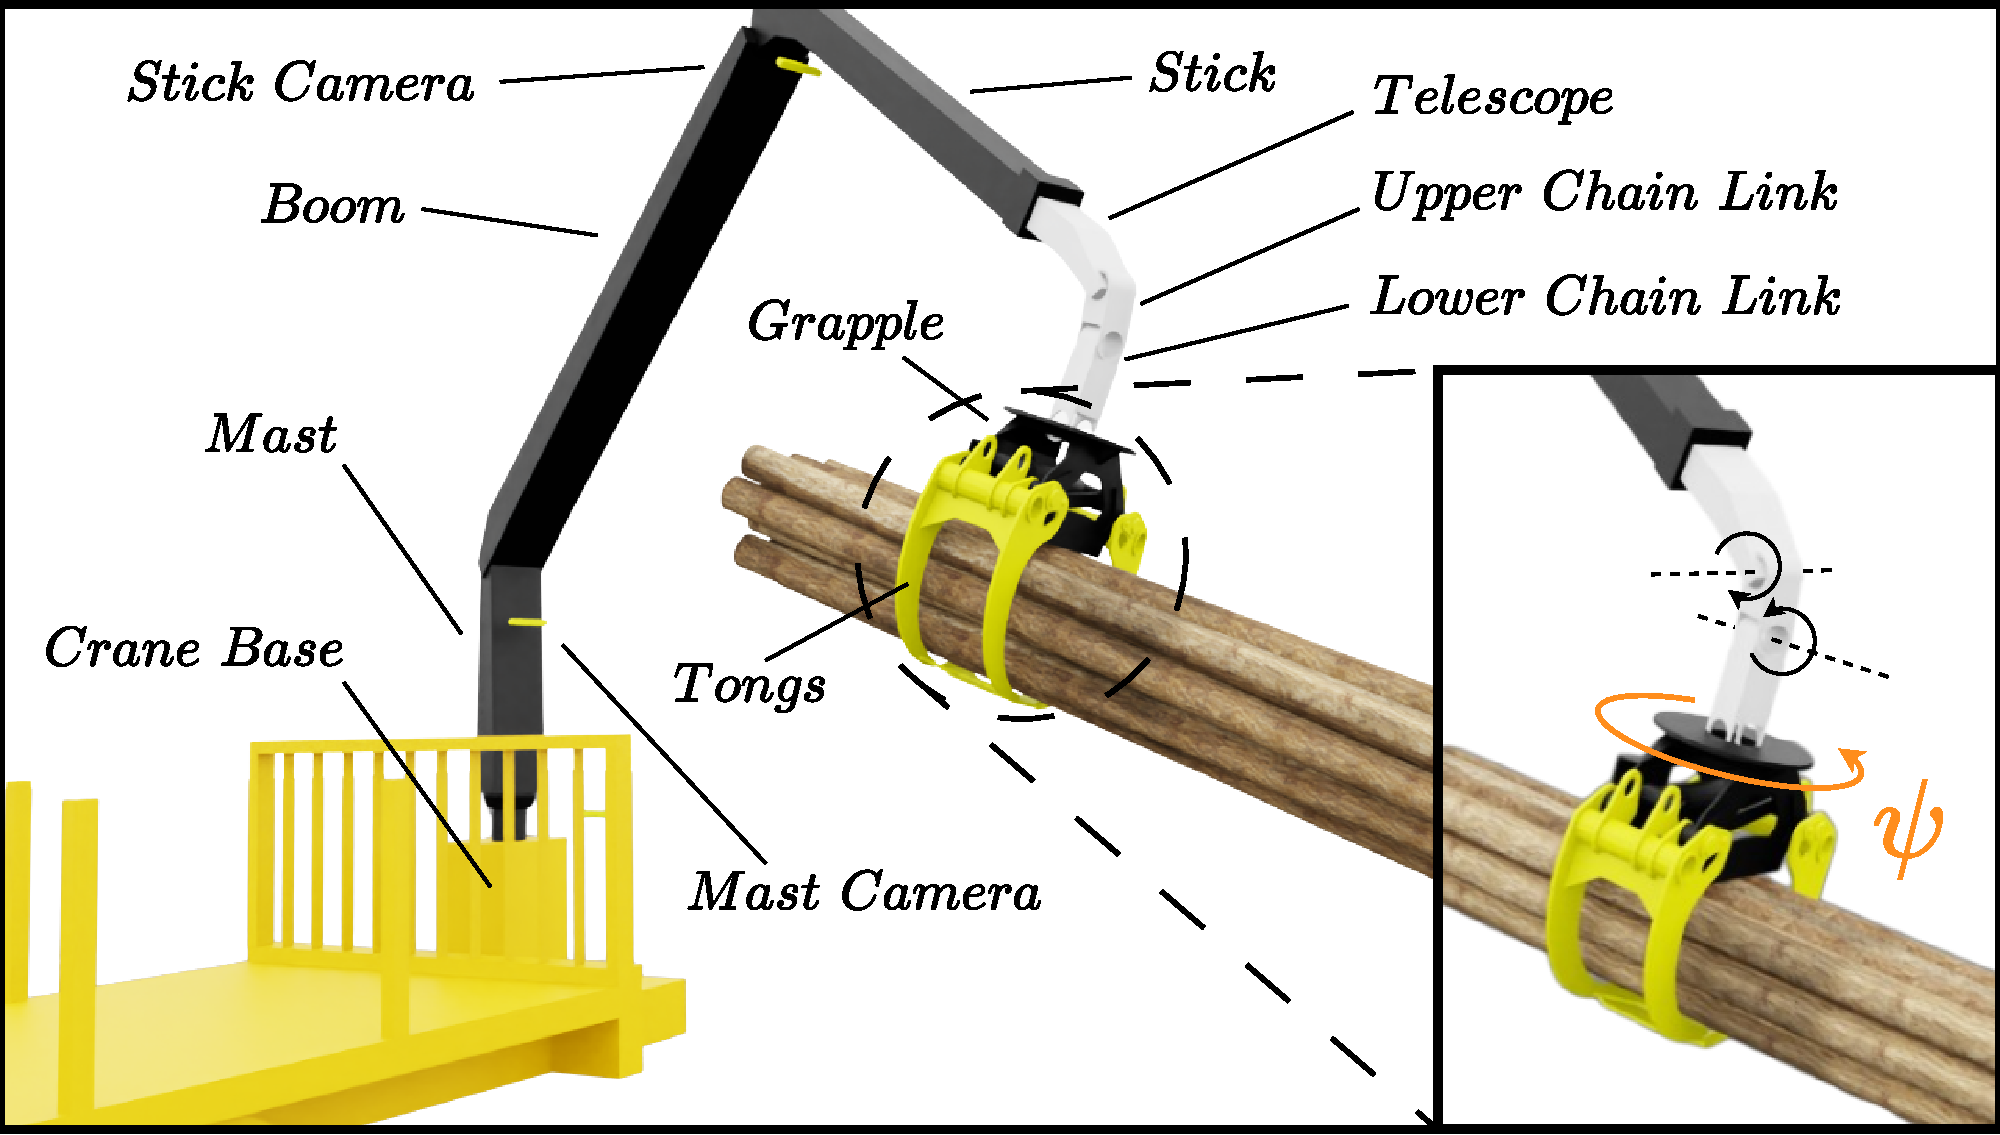
\includegraphics[width=\linewidth]{crane_links.pdf}
\caption{The simulated crane and its links. The four actuated arm joints
(slew at the crane base, boom, stick, telescope) carry a two-link passive
chain, below which the grapple yaw joint and the tongs act. Inset: the
passive chain pivots freely in two axes, so the grapple hangs under gravity
and swings during arm motion, while the yaw joint sets the grapple heading
$\psi$. The two stereo cameras are shown at the mounts they occupy on the
physical machine (Chapter~\ref{ch:sim2real}).}
\label{fig:sim_crane_links}
\end{figure}

\begin{figure}[t]
\centering
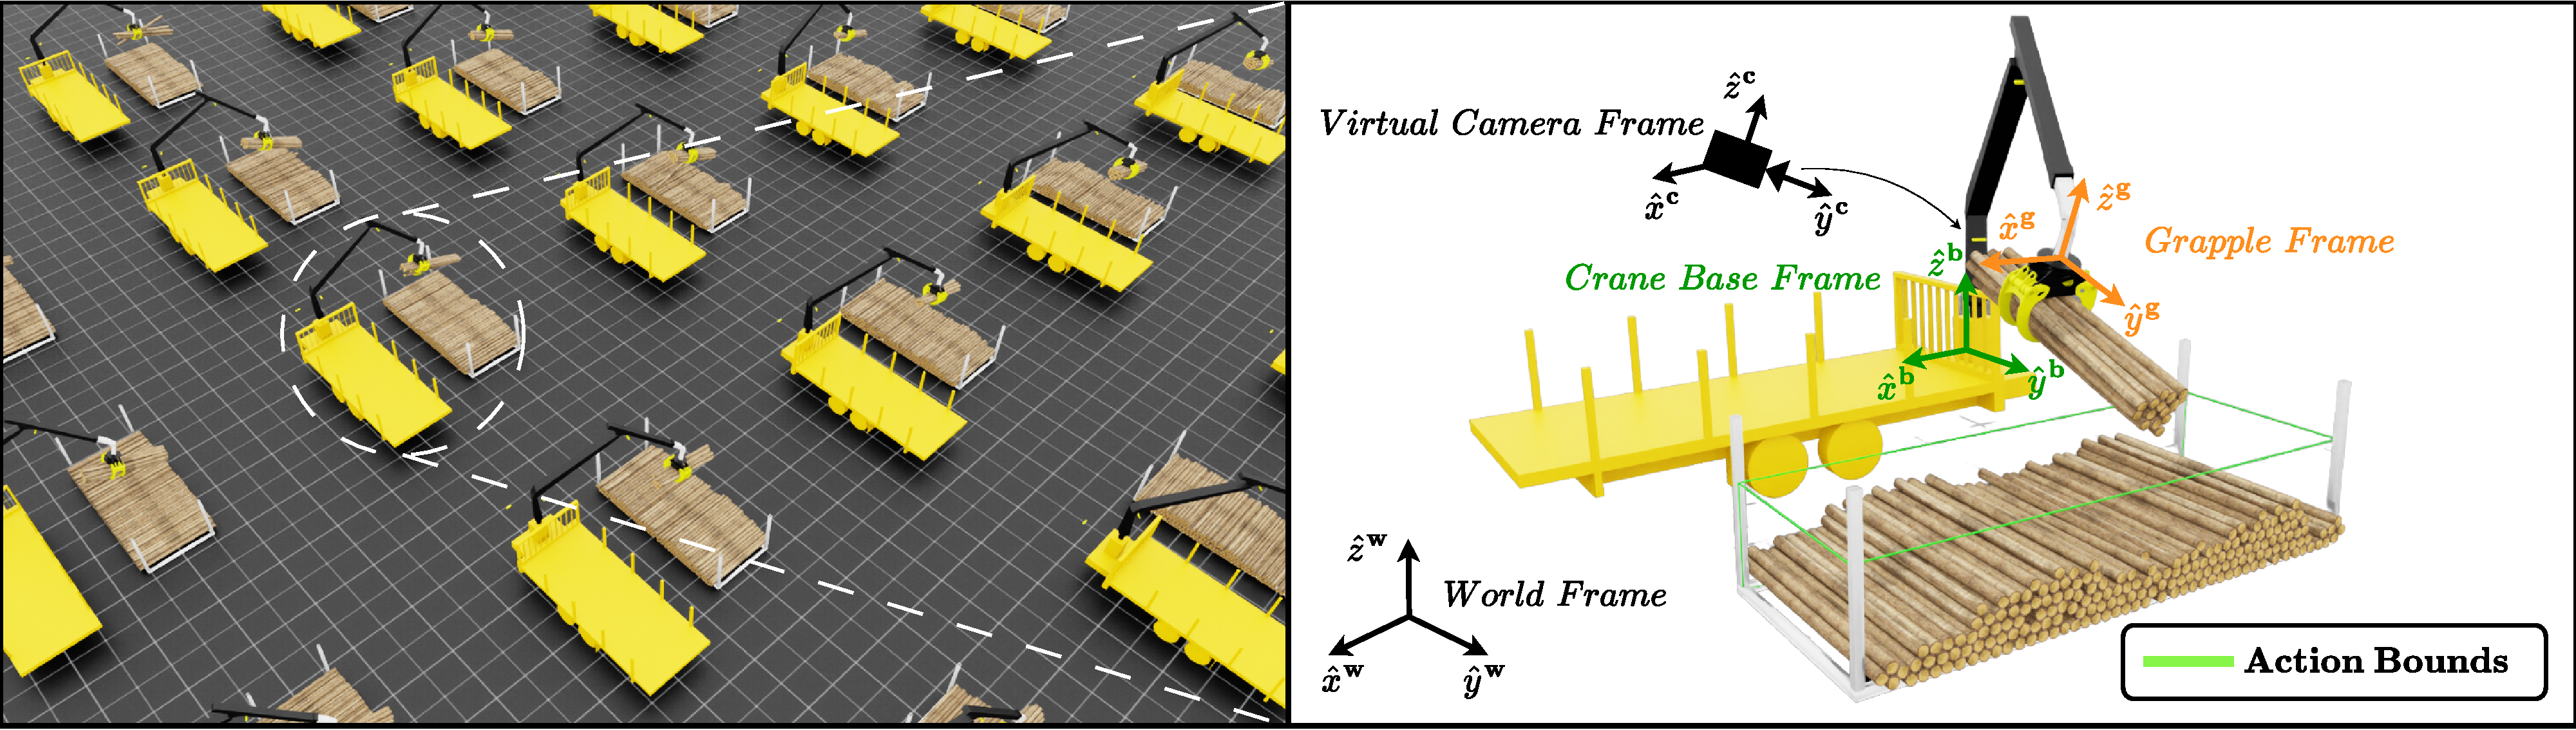
\includegraphics[width=\linewidth]{crane_env_basemast.pdf}
\caption{The simulated testbed. Left: parallel environment instances, each
with an independently randomized pile, stepped together on the GPU. Right: a
single environment with the frames the task is expressed in. The policy
observes a point cloud and selects a grasp target inside the rack-aligned
action volume (green), and a fixed state machine executes the cycle.}
\label{fig:sim_env_scene}
\end{figure}

The passive chain deserves emphasis because it shapes both control and
evaluation. Because the grapple is not rigidly attached, every commanded
motion excites swing that must decay before a grasp can be executed
accurately, and the tilt of the suspended load after lifting is the physical
signal behind the stability metric of Section~\ref{sec:sim_outcome}. The
fidelity of the chain's spring-damper model turned out to matter: the values
used during the early simulation campaigns (stiffness 300, damping 500 in the
chain joints) suppress swing more strongly than the real, freely pivoting
hanger, with consequences for stability measurements that are taken up in
Section~\ref{sec:sim_study_stability} and Chapter~\ref{ch:sim2real}. The
corrected configuration frees the pivots (zero stiffness with light damping).

\section{Physics Modeling and Tuning}

Simulating a dense pile is a different regime from typical robotics scenes:
several hundred rigid bodies rest in persistent frictional contact, and the
grapple deliberately drives into the contact network. Default physics
settings failed outright, with logs ricocheting on spawn, chain-reaction
pile explosions on grapple contact, and scene crashes beyond roughly 300
bodies. The configuration below was reached by systematic tuning on the
original Isaac Sim implementation of the scene and is inherited by the Isaac
Lab environment, which reuses the same assets and physics parameters.

\subsection{Log assets from field measurements}

Log geometry and mass follow direct measurements of ten logs at the
FPInnovations testbed (Table~\ref{tab:log_measurements}). The simulation log
is a cylinder of diameter 0.113~m and length 2.45~m with a mass of 15~kg,
matching the measured averages. Logs are instanced from a single prototype
asset~\cite{blender, nvidia_instancing}, which keeps memory usage flat in the
number of logs, guarantees identical physical properties across instances,
and lets material or collision changes be applied globally during tuning.

\begin{table}[t]
\centering
\caption{Field measurements of the testbed logs (two end diameters D1, D2).
The simulated log uses the rounded averages: diameter 0.113~m, length 2.45~m,
mass 15~kg.}
\label{tab:log_measurements}
\begin{tabular}{ccccc}
\hline
\textbf{Log} & \textbf{D1 (mm)} & \textbf{D2 (mm)} & \textbf{Length (mm)} & \textbf{Mass (kg)} \\
\hline
1 & 101 & 86 & 2480 & 12.2 \\
2 & 104 & 123 & 2390 & 14.2 \\
3 & 72 & 113 & 2600 & 11.8 \\
4 & 120 & 132 & 2480 & 17.4 \\
5 & 121 & 94 & 2560 & 15.6 \\
6 & 124 & 142 & 2450 & 18.1 \\
7 & 110 & 129 & 2550 & 18.0 \\
8 & 89 & 110 & 2550 & 9.7 \\
9 & 126 & 110 & 2290 & 15.8 \\
10 & 136 & 114 & 2180 & 15.6 \\
\hline
Mean & 110.3 & 115.3 & 2453 & 14.8 \\
\hline
\end{tabular}
\end{table}

Contact material properties use published oak-on-oak friction coefficients
($\mu_s = 0.62$, $\mu_k = 0.48$)~\cite{avallone2006marks} with near-zero
restitution (0.05) so that impacts dissipate energy. Friction combines by
maximum and restitution by minimum across contact pairs~\cite{nvidia_combine},
the conservative choices for stability. With these values, spawned logs settle
into piles with realistic angles of repose, grasped bundles cohere through
friction during transport, and released logs come to rest within one to two
seconds without bouncing.

\subsection{Collision geometry and detection}

Collision representations are chosen per component~\cite{nvidia_colliders}:
convex hulls for logs (an efficient 32-vertex cylinder approximation), convex
decomposition for the rack so its concave cradle actually contains logs, and
signed-distance-field (SDF) meshes for the grapple tongs, whose curved,
interlocking geometry needs smooth contact normals for multi-log grasps to
close reliably. Continuous collision detection is enabled for logs and
grapple parts~\cite{nvidia_ccd}, eliminating tunneling during pile settling,
fast approaches, and log release.

\subsection{Solver}

The constraint solver choice proved decisive. The default temporal
Gauss-Seidel (TGS) solver became less stable as iterations increased: its
aggressive convergence injects energy when resolving the deep
interpenetrations that arise inside dense piles, producing explosive
collapses. The projected Gauss-Seidel (PGS) solver, with high position and
velocity iteration counts, resolves the same contact networks
conservatively~\cite{nvidia_solver} and is used throughout. Physics runs at
120~Hz with a control decimation of two (60~Hz control).

\subsection{Actuation and pile initialization}

Actuated joints use implicit PhysX PD drives ($k_p = 10^6$,
$k_d = 10^5$)~\cite{nvidia_joints}, with torque limits sized from the loads of
multi-log lifts; the grapple yaw joint and tongs use lower gains, with the
tongs driven by a saturated PD velocity law with discrete stepping to avoid
abrupt contact forces. Piles are initialized by spawning logs in a layered
grid above the rack with small random perturbations, then simulating until
maximum linear and angular velocities fall below thresholds; the settled
configuration becomes the episode's initial state. Randomization over log
count, grid dimensions, spacing, layer offsets, and per-log jitter (and, in
later data-collection recipes, profiled mound shapes) generates pile
diversity across episodes.

\begin{table}[t]
\centering
\caption{Principal simulation and controller parameters. Actuator gains are
implicit PhysX joint-drive values. The passive-chain values in parentheses are
the corrected free-pivot configuration adopted after hardware comparison
(Section~\ref{sec:sim_study_stability}).}
\label{tab:sim_params}
\small
\begin{tabular}{lr}
\hline
\textit{Simulation} & \\
Physics timestep & $1/120$ s \\
Control decimation & $2\times$ (60 Hz) \\
\hline
\textit{Crane link masses} & \\
Mast / main boom / stick & 290 / 172 / 70 kg \\
Telescope / passive chain links & 25 / 9 kg \\
\hline
\textit{Joint limits} & \\
Base-mast (revolute) & $\pm 100^{\circ}$ \\
Boom (revolute) & $-22^{\circ}$ to $+75^{\circ}$ \\
Stick (revolute) & $-177^{\circ}$ to $+2^{\circ}$ \\
Telescope (prismatic) & 0.13--1.80 m \\
Grapple yaw (revolute) & $\pm 180^{\circ}$ \\
\hline
\textit{Actuator gains} ($k_p$ / $k_d$) & \\
Main arm joints & $10^{6}$ / $10^{5}$ \\
Passive chain & 300 / 500 \; (corrected: 0 / 100) \\
Grapple yaw & $5\times 10^{4}$ / $2\times 10^{4}$ \\
Grapple tongs & 0 / 500 \\
\hline
\textit{Log properties} & \\
Diameter / length & 0.113 / 2.45 m \\
Mass & 15 kg \\
Friction $\mu_s$ / $\mu_k$ & 0.62 / 0.48 \\
Restitution & 0.05 \\
Contact / rest offset & 0.02 / 0.0 m \\
\hline
\textit{FSM parameters} & \\
Hover clearance & 2.5 m \\
Position tolerance (chain top / grapple) & 0.10 / 0.25 m \\
Dwell count & 30 steps \\
Phase timeout & 100 steps \\
\hline
\end{tabular}
\end{table}

\section{The Grasp-Cycle State Machine}
\label{sec:sim_fsm}

All methods in this thesis, heuristic and learned alike, share one fixed
execution controller: a finite state machine (FSM) that turns a commanded
grasp target $(x, y, z, \psi)$ into a complete grasp cycle. The arm is driven
by Isaac Lab's damped-least-squares differential inverse-kinematics
controller in task space; the grapple yaw joint is position-controlled
independently. Because the IK target is the top of the passive chain while
the grasp happens at the grapple body hanging below it, targets are specified
for the grapple and offset vertically to the IK link, and each phase uses a
two-stage convergence check: the IK link must reach its target within
0.10~m, then the grapple body must settle within 0.25~m, both holding for 30
consecutive steps so that pendulum oscillation has died out before the cycle
proceeds. A per-phase timeout forces advancement if convergence is not
reached, preventing stalls on difficult configurations.

The cycle has five phases: \texttt{HOVER} moves the grapple above the target
with 2.5~m clearance; \texttt{ALIGN} rotates the grapple to the commanded
yaw; \texttt{DESCEND} lowers it at reduced speed to limit pile disturbance;
\texttt{CLOSE} shuts the jaws with discrete velocity stepping; and
\texttt{LIFT} raises the load back to hover height and holds it while the
grasp outcome is evaluated. In the grasp-and-remove configuration used for
the simulation study of Chapter~\ref{ch:sim_study}, grasped logs are then
removed from the scene and the cycle repeats; the environment also supports
full transport-and-deposit cycles, which are used in the deployment-aligned
configuration of Chapter~\ref{ch:sim2real}.
Algorithm~\ref{alg:fsm} states the cycle; parameter values are in
Table~\ref{tab:sim_params}.

\begin{algorithm}[t]
\caption{Grasp-cycle state machine, shared by every method in this thesis}
\label{alg:fsm}
\begin{algorithmic}
\algin{Grasp target $\mathbf{g} = (x, y, z, \psi)$; hover clearance $h$;
tolerances $\epsilon_{\mathrm{ik}}$ (chain top) and $\epsilon_{\mathrm{gr}}$
(grapple body); dwell count $D$; per-phase timeout $T_{\max}$.}
\algout{Cycle outcome $(n, \alpha, \varsigma)$ of Section~\ref{sec:sim_outcome}.}

\Function{Settle}{target $\mathbf{p}$}
  \Comment{two-stage convergence, run every control step}
  \State Command the chain-top IK link to $\mathbf{p}$ offset vertically for the hanging grapple
  \State Wait until $\lVert \mathbf{p}_{\mathrm{ik}} - \mathbf{p} \rVert < \epsilon_{\mathrm{ik}}$,
         \textbf{then} until $\lVert \mathbf{p}_{\mathrm{grapple}} - \mathbf{p} \rVert < \epsilon_{\mathrm{gr}}$
  \State Require both to hold for $D$ consecutive steps
  \Comment{lets swing decay first}
  \State Advance regardless after $T_{\max}$ steps
  \Comment{timeout prevents stalls}
\EndFunction

\algstage{1.\;\texttt{HOVER}}
\State \Call{Settle}{$(x, y, z + h)$}

\algstage{2.\;\texttt{ALIGN}}
\State Drive the grapple yaw joint to $\psi$ and hold position

\algstage{3.\;\texttt{DESCEND}}
\State \Call{Settle}{$(x, y, z)$} at reduced command scale
\Comment{limits pile disturbance}

\algstage{4.\;\texttt{CLOSE}}
\State Close the tongs under a saturated velocity law with discrete stepping

\algstage{5.\;\texttt{LIFT}}
\State Raise to $(x, y, z + h)$ and hold while the load settles
\State Evaluate the outcome: throughput $n$, alignment $\alpha$, stability $\varsigma$
\State Remove grasped logs (grasp-and-remove) or continue to transport and release
\State \Return $(n, \alpha, \varsigma)$
\end{algorithmic}
\end{algorithm}

\section{Task Formulation}
\label{sec:sim_task}

\subsection{A decision-level MDP}

The learning problem is formulated at the level of grasp decisions rather
than joint commands: one environment step is one complete grasp cycle, an
abstraction in the spirit of temporally extended
actions~\cite{sutton1999between}. The state is the pile configuration,
observed either as a point cloud or, for privileged baselines, as log poses;
the action is the grasp target; the transition is whatever the physics and
the FSM produce; and one scalar reward summarizes the cycle's outcome. An
episode ends when the rack is empty or after a fixed budget of $H = 30$ grasp
attempts, chosen with roughly 50\% margin over what the scripted expert needs
to clear a 200-log pile. Horizons of tens of decisions, rather than
thousands of control steps, are what make on-policy fine-tuning with a
privileged critic practical in Chapters~\ref{ch:sim_study} and \ref{ch:bcrl}.

\subsection{Observations}
\label{sec:sim_obs}

The policy observes a point cloud derived from a simulated depth camera
above the rack, with pinhole intrinsics matching the Stereolabs ZED~X used on
the physical testbed. Valid depth pixels are back-projected through the
intrinsics, transformed into the crane base frame using the known camera
extrinsics, cropped to a box around the rack, and downsampled with farthest
point sampling (FPS) to a fixed budget of $N$ points (1024 in the simulation
study; 2048 in the widened deployment pipeline of
Chapter~\ref{ch:bc_policies}); short clouds are zero-padded.
Algorithm~\ref{alg:obs_pipeline} states the procedure, and
Figure~\ref{fig:sim_pcd_pipeline} shows it applied to one decision.
Critically, no segmentation is applied at any stage: the cloud contains every
surface the camera sees, including rack structure and ground, and the
network must learn what is graspable. As a privileged ablation, some
baselines instead observe the top-$K$ log poses ($K = 32$), height-sorted, as
a compact $4K$-dimensional vector $\xi_t$; the comparison isolates the cost of
perception from the learning algorithm.

The same procedure runs at deployment, with the simulated camera replaced by
the physical one and the known extrinsics replaced by the calibrated mount of
Section~\ref{sec:s2r_camcalib}. Keeping it operation for operation identical
is a hard requirement rather than a convenience: any step that differs
between the two is a distribution shift the policy pays for directly, so
Algorithm~\ref{alg:obs_pipeline} is the single definition referenced by both
the training pipelines of Chapter~\ref{ch:bc_policies} and the deployed node
of Section~\ref{sec:s2r_deploy}.

\begin{algorithm}[t]
\caption{Observation pipeline (identical in simulation and at deployment)}
\label{alg:obs_pipeline}
\begin{algorithmic}
\algin{Depth image $Z$ with pinhole intrinsics $K_{\mathrm{cam}}$; extrinsic
$T_{\mathrm{base} \leftarrow \mathrm{cam}}$; action box
$[b^{\min}, b^{\max}]$; crop margin $m$; point budget $N$.}
\algout{Observation cloud $P \in \mathbb{R}^{N \times 3}$ in the crane base
frame, with a padding mask.}

\algstage{1.\;Back-projection}
\State Discard invalid depth pixels; back-project the rest through
$K_{\mathrm{cam}}$ to camera-frame points $P_{\mathrm{raw}}$.

\algstage{2.\;Base-frame transform}
\State $P \gets T_{\mathrm{base} \leftarrow \mathrm{cam}}\, P_{\mathrm{raw}}$
\Comment{known in simulation, calibrated on the crane}

\algstage{3.\;Crop}
\State $P \gets \{\, p \in P \;:\; b^{\min} - m \preceq p \preceq b^{\max} + m \,\}$
\Comment{no segmentation; structure and ground are kept}

\algstage{4.\;Resample to a fixed budget}
\If{$|P| > N$}
  \State $P \gets \mathrm{FPS}_N(P)$ \Comment{farthest point sampling}
\Else
  \State Zero-pad $P$ to $N$ rows and mark the padded slots
\EndIf
\State \Return $P$ and the padding mask
\end{algorithmic}
\end{algorithm}

\begin{figure}[t]
\centering
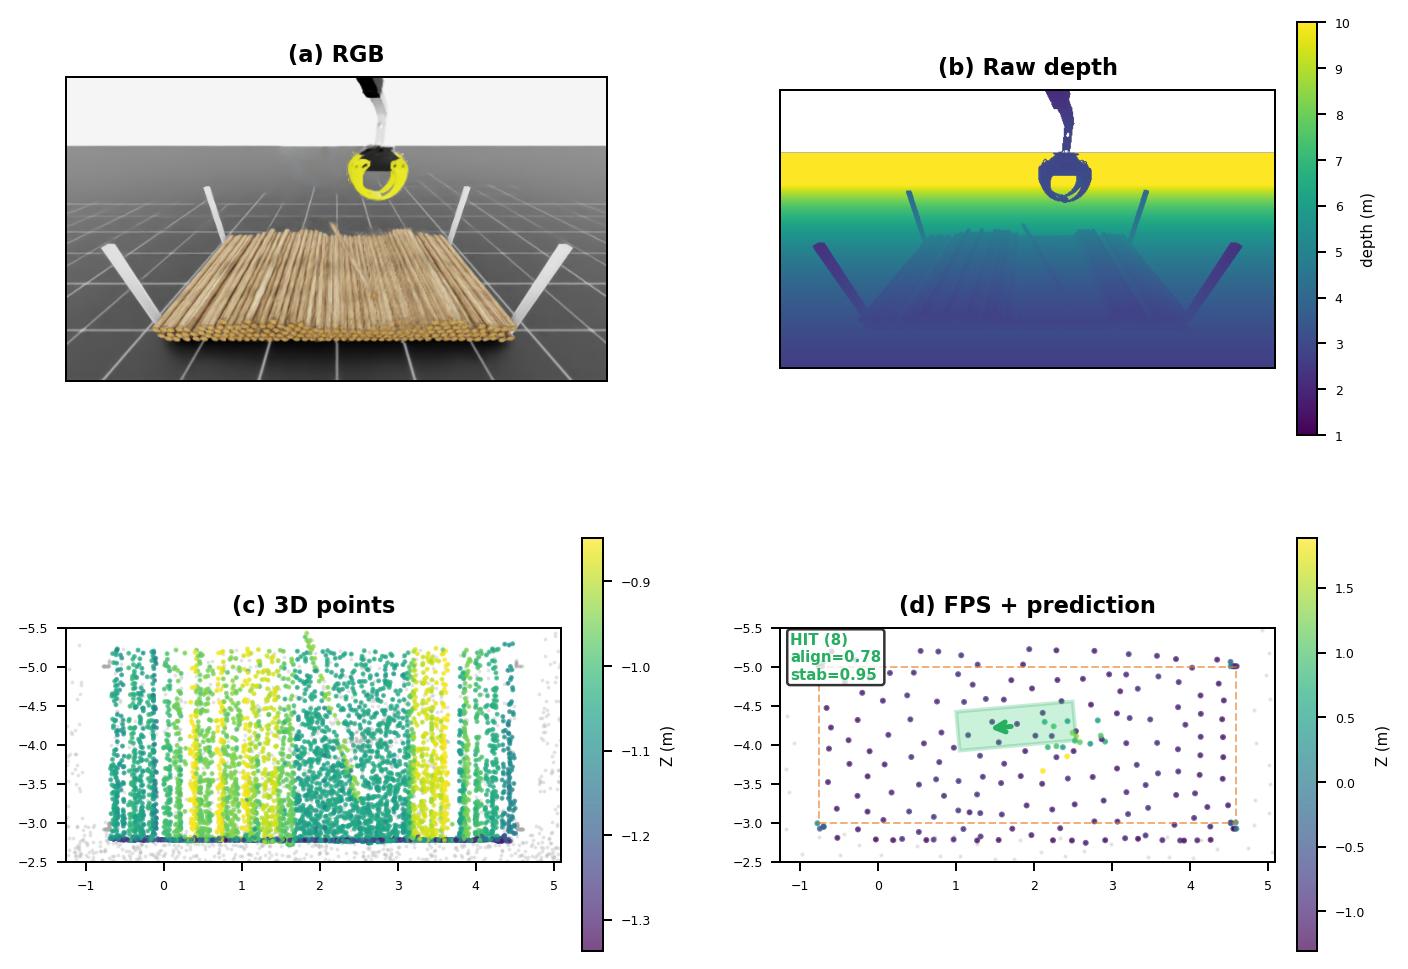
\includegraphics[width=\linewidth]{episode_001_pipeline_quad_single.png}
\caption{Observation pipeline for a single grasp decision. (a)~Camera RGB
view, (b)~raw depth, (c)~3D back-projection in the crane base frame,
(d)~FPS-downsampled point cloud with the policy's grasp target and the
grapple footprint overlaid.}
\label{fig:sim_pcd_pipeline}
\end{figure}

\subsection{Actions}
\label{sec:sim_actions}

A grasp target is the tuple $\mathbf{g} = (x, y, z, \psi)$: the grapple
position in the crane base frame and its yaw about the vertical axis
(Figure~\ref{fig:sim_env_scene}). Learned policies output five unbounded
scalars. The three position components are squashed by $\tanh$ and mapped
linearly into a rack-aligned action box, so every decodable action is a
physically executable target; the box also serves
as the out-of-bounds cull region for logs knocked off the rack. Yaw is
represented by the doubled-angle pair $(\cos 2\psi, \sin 2\psi)$: a
cylindrical log at yaw $\psi$ is identical at $\psi + \pi$, and the
$\pi$-periodic encoding maps the two physically identical grasps to the same
point~\cite{morrison2018closing}, which proves essential for supervised
training (Chapter~\ref{ch:bc_policies}). Expert targets are encoded into the
same pre-squash space, so imitation and reinforcement learning share one
action space.

\subsection{Outcome evaluation}
\label{sec:sim_outcome}

After the lift, the outcome of the cycle is measured by three quantities.
The \emph{throughput} $n$ counts the logs held by the grapple (centers within
a proximity radius). The \emph{alignment}
\begin{equation}
  \alpha_i = \big( \hat{y}_g^{\top} \hat{y}_{\ell_i} \big)^{8}, \qquad
  \alpha = \frac{1}{n} \sum_{i=1}^{n} \alpha_i \in [0, 1],
\end{equation}
scores the angle between the grapple jaw axis $\hat{y}_g$ and each held log's
length axis $\hat{y}_{\ell_i}$; the even exponent absorbs the log's
directional symmetry and the eighth power penalizes moderate misalignment
sharply. The \emph{stability}
\begin{equation}
  \varsigma = \big( \max(0,\; \hat{z}_g^{\top} \hat{z}_w) \big)^{4} \in [0, 1]
  \label{eq:sim_stability}
\end{equation}
scores the levelness of the grapple after lifting, with $\hat{z}_g$ its up
vector and $\hat{z}_w$ the world vertical. Figure~\ref{fig:sim_outcomes}
shows the shaped score curves.

Equation~\eqref{eq:sim_stability} is the \emph{snapshot} form, evaluated from
a single sample at the end of a fixed hold, which is how the metric was
implemented for the campaigns of Chapter~\ref{ch:sim_study}. It was later
replaced by a \emph{windowed} form that mirrors the measurement procedure
running on the physical crane. Writing
$\theta_t = \arccos\big(\max(0,\; \hat{z}_g^{\top} \hat{z}_w)\big)$ for the
tilt sampled at control step $t$ of the post-lift hold,
\begin{equation}
  \varsigma = \big( \cos \bar{\theta} \big)^{4}, \qquad
  \bar{\theta} = \frac{1}{|W|} \sum_{t \in W} \theta_t ,
  \label{eq:sim_stability_windowed}
\end{equation}
where $W$ is the trailing one-second window of the hold, accepted once its
variance stays below $10^{-4}$~rad$^2$ for half a second and otherwise taken
best-effort at a four-second timeout. Averaging the angle before sharpening,
rather than sharpening each sample, keeps the score independent of the
sampling rate and so comparable to the crane's timer-paced measurement; the
clamp inside $\theta_t$ bounds each sample to $[0, \pi/2]$, which is why no
outer clamp is needed in
Equation~\eqref{eq:sim_stability_windowed}. Both forms use the same exponent
and share the interpretation of Figure~\ref{fig:sim_outcomes}; the windowed
form is the one used for the reward and the reported metric in
Chapters~\ref{ch:bc_policies} and~\ref{ch:bcrl}. Which form is in force is
recorded with each result, because the two are not interchangeable: a
snapshot can catch the load at any point of a residual swing, whereas the
windowed value only reports once the swing has actually decayed. That is a
separate issue from the passive-chain modeling error that led one campaign's
stability results to be withdrawn (Section~\ref{sec:sim_study_stability}).

Reported quantities also include the grasp success rate (fraction of cycles
with $n > 0$), the pile clearing rate (fraction of the initial inventory
intentionally grasped and removed), and the fraction of logs knocked out of
bounds.

\begin{figure}[t]
\centering

\includegraphics[width=\linewidth]{outcomes.png}
\caption{Grasp outcome geometry and shaped scores. The per-log misalignment
angle $\theta_{\alpha_i}$ is measured between the grapple closing axis
$\hat{y}_g$ and the log axis $\hat{y}_{\ell_i}$, and the tilt angle
$\theta_\varsigma$ between the grapple vertical $\hat{z}_g$ and the world
vertical. Insets: the shaped alignment score
$\alpha_i = (\cos\theta_{\alpha_i})^8$ and stability score
$\varsigma = (\max(0, \cos\theta_\varsigma))^4$; the sharp exponents
concentrate reward on well-aligned, level grasps.}
\label{fig:sim_outcomes}
\end{figure}

\section{The Privileged Heuristic Expert}
\label{sec:sim_expert}

A scripted expert serves as both a competitive baseline and the
demonstration source for behavior cloning. It has privileged access to the
poses of all active logs and follows a top-of-pile targeting strategy: at
each cycle it selects the log with the highest center, targets that center,
and aligns the grapple yaw with the log's length axis, choosing between the
two symmetric orientations by minimal joint rotation and re-evaluating the
alignment closed-loop during the \texttt{ALIGN} phase
(Algorithm~\ref{alg:expert}). The highest log is
typically the most accessible, with the fewest obstructing neighbors, and
executing this strategy clears 200-log piles reliably in roughly 20 cycles.
Its known weakness is the endgame: when few scattered logs remain, the
highest point is no longer clearly the best target, and on the real machine
the same rule can lock onto rack structure once the pile falls below the rail
height, a failure mode measured and addressed in
Chapter~\ref{ch:bc_policies}.

\begin{algorithm}[t]
\caption{Privileged heuristic expert (top-of-pile targeting)}
\label{alg:expert}
\begin{algorithmic}
\algin{Ground-truth poses of the active logs $\ell_1, \dots, \ell_L$ (centers
$c_j$ and length axes $\hat{y}_{\ell_j}$), read from the simulator; current
grapple yaw $\psi_0$.}
\algout{Grasp target $\mathbf{g} = (x, y, z, \psi)$ for
Algorithm~\ref{alg:fsm}.}

\State $j^{*} \gets \operatorname*{arg\,max}_{j} \; c_{j,z}$
\Comment{topmost log: fewest obstructing neighbors}
\State $(x, y, z) \gets c_{j^{*}}$
\Comment{target the log center, not its surface}
\State $\psi_{\mathrm{raw}} \gets \operatorname{atan2}\big(\hat{y}_{\ell_{j^{*}},y},\; \hat{y}_{\ell_{j^{*}},x}\big)$
\Comment{align the jaws across the log axis}
\State $\psi \gets \operatorname*{arg\,min}_{\phi \,\in\, \{\psi_{\mathrm{raw}},\; \psi_{\mathrm{raw}} + \pi\}}
        \; |\phi - \psi_0|$
\Comment{$\pi$-symmetric; pick the shorter rotation}
\State \Return $(x, y, z, \psi)$, re-evaluating $\psi$ closed-loop during \texttt{ALIGN}
\end{algorithmic}
\end{algorithm}

\section{Summary}

The testbed simulates the physical log-loader at pile scale: a crane with a
passively suspended grapple, racks of approximately 200 field-measured logs in
frictional contact, and physics tuned (conservative PGS solving, SDF tong
collision, CCD, measured friction) until pile behavior is stable and
plausible. A fixed FSM executes complete grasp cycles from commanded targets,
isolating the learned decision from motion execution, and the task is
formulated as a decision-level MDP over grasp targets with per-cycle outcome
scores. The next chapter uses this testbed to compare learning methods for
the targeting decision.

% Thesis chapter: simulation study comparing heuristic, RL, BC, and BC->RL.
% Standalone chapter file; \input or \include from the thesis root.
% Distills the IROS draft results with the stability-metric caveat applied:
% stability numbers from this campaign (overdamped passive chain) are not
% reported, and no stability-improvement claim is made.

\chapter{Learning to Clear Piles in Simulation}
\label{ch:sim_study}

This chapter asks the first question of the thesis: can a policy learn
sequential grasp targeting for dense piles from raw point clouds, and what
combination of learning methods gets it there? Four methods are compared on
the testbed of Chapter~\ref{ch:sim_env} under one shared controller, pile
distribution, and evaluation protocol: the privileged heuristic expert,
reinforcement learning from scratch, behavior cloning of the expert, and
behavior cloning followed by reinforcement learning fine-tuning. The result
that organizes everything downstream is a clean dissociation: from-scratch RL
fails at the trajectory level regardless of what it observes, behavior
cloning from raw clouds reaches near-expert clearing, and a carefully
constrained fine-tuning recipe preserves that competence while optimizing
per-grasp execution.

\section{Behavior Cloning}
\label{sec:study_bc}

Demonstrations are collected by running the privileged expert of
Section~\ref{sec:sim_expert} and recording, for each successful grasp, the
point cloud observation and the expert action encoded in the policy's action
space (positions through the inverse squashing map, yaw as the doubled-angle
pair). Failed grasps are discarded. The dataset used here contains roughly
20{,}700 successful-grasp samples with an 85/15 train/validation split.

The policy is a PointNet encoder~\cite{qi2017pointnet} followed by a small
actor head. A shared per-point multilayer perceptron
($3 \to 64 \to 128 \to 256$, batch normalization, ELU
activations~\cite{clevert2015elu}) maps each point independently; a
channelwise max-pool aggregates the set; a fully connected layer produces a
256-dimensional global feature; and an actor MLP
($256 \to 128 \to 64 \to 5$) with dropout 0.2 outputs the action. Training
minimizes mean-squared error against the expert action with
AdamW~\cite{loshchilov2019adamw} (learning rate $10^{-4}$, weight decay
$10^{-4}$), plateau scheduling, and early stopping on validation loss. For
the privileged-pose ablation the encoder is replaced by an MLP on the
128-dimensional pose vector.

\section{Reinforcement Learning from Scratch}
\label{sec:study_rl}

The RL baselines are trained with proximal policy
optimization~\cite{schulman2017ppo} in the RSL-RL
library~\cite{schwarke2025rslrl}, using a Gaussian policy over the same 5D
action space and a symmetric actor-critic: actor and critic each process the
observation through their own encoder (PointNet for cloud inputs, MLPs for
the pose ablation), so the value gradient doubles as an auxiliary
representation-learning signal. The reward is the per-cycle outcome product
\begin{equation}
  r = n \cdot \alpha \cdot \varsigma
  \label{eq:study_reward}
\end{equation}
for successful grasps and $r = -1$ for failures, where $n$, $\alpha$, and
$\varsigma$ are the throughput, alignment, and stability scores of
Section~\ref{sec:sim_outcome}. The reward is entirely per-grasp: any
trajectory-level clearing competence must emerge from targeting strategy
rather than from explicit shaping. Key settings: initial policy standard
deviation $\sigma_0 = 1.0$, clip 0.2, entropy coefficient 0.01, learning rate
$3 \times 10^{-4}$ with adaptive KL scheduling (target 0.01), generalized
advantage estimation ($\lambda = 0.95$), and discount $\gamma = 0.99$.

\section{BC-Initialized Fine-Tuning}
\label{sec:study_bcrl}

The fine-tuned policy loads the trained BC actor (encoder and head) into the
PPO actor and continues training on-policy~\cite{rajeswaran2018learning,
nair2018overcoming}, with three deliberate constraints
(Figure~\ref{fig:study_pipeline}).

First, the critic is \emph{asymmetric}~\cite{pinto2018asymmetric}: it is a
freshly initialized MLP on the privileged 128-dimensional pose state rather
than on the point cloud. It learns an accurate value function within a few
iterations, precisely because it does not need to learn perception, and it
shares no parameters with the actor.

Second, the BC-trained PointNet encoder is \emph{frozen}. The state-based
critic cannot propagate gradients through the visual pathway, so an unfrozen
encoder would drift without constraint; in practice, fine-tuning the full
network collapses training (Figure~\ref{fig:study_ablation}).

Third, exploration starts \emph{small}: $\sigma_0 = 0.05$ instead of 1.0,
restricting early rollouts to small perturbations around the BC policy's
actions. Higher noise degrades the initialization faster than reward feedback
can compensate, gradually at $\sigma_0 = 0.1$ and rapidly at
$\sigma_0 = 0.3$ (Figure~\ref{fig:study_ablation}). All other
hyperparameters match the from-scratch configuration. Because return degrades
late in long fine-tunes, the evaluation checkpoint is selected by early
stopping.

\begin{figure}[t]
\centering

\includegraphics[width=\linewidth]{bcrl_ablation_minimal.pdf}
\caption{Fine-tuning sensitivity. Mean episode return against PPO iteration
for four configurations varying encoder freezing and initial exploration
noise $\sigma_0$. Only the frozen-encoder, $\sigma_0 = 0.05$ configuration
sustains performance; unfreezing the encoder collapses training regardless of
noise level, and larger $\sigma_0$ degrades the BC initialization gradually
(0.1) or rapidly (0.3).}
\label{fig:study_ablation}
\end{figure}

\begin{figure}[t]
\centering
\resizebox{\linewidth}{!}{%
\begin{tikzpicture}[
  block/.style={rectangle, rounded corners=3pt, draw=black!70,
    text width=3.0cm, minimum height=0.7cm, align=center,
    font=\scriptsize, inner sep=4pt},
  frozen/.style={block, fill=blue!12},
  trainable/.style={block, fill=orange!18},
  io/.style={block, fill=white},
  lossnode/.style={rectangle, rounded corners=3pt, draw=black!50, dashed,
    text width=3.4cm, align=center, font=\scriptsize, inner sep=4pt, fill=gray!5},
  wideloss/.style={lossnode, text width=5.5cm},
  arr/.style={-{Stealth[length=4pt]}, thick, black!70},
  panelbg/.style={rectangle, rounded corners=6pt, draw=gray!50,
    fill=gray!3, inner sep=8pt},
  ptitle/.style={font=\small\bfseries},
  collabel/.style={font=\scriptsize\itshape, text=black!60},
]
% ====== PANEL (a): BEHAVIOR CLONING ======
\node[io] (a_pcd) at (0, 0)
  {Raw cloud\\$P_t \in \mathbb{R}^{1024\times3}$};
\node[io] (a_expert) at (4, 0)
  {Expert heuristic\\$a^{*} \in \mathbb{R}^{5}$};
\node[trainable, below=0.25cm of a_pcd] (a_enc)
  {PointNet encoder\\$3\!\to\!64\!\to\!128\!\to\!256$\\BN + ELU, max-pool\\$\to\mathbb{R}^{256}$};
\node[trainable, below=0.25cm of a_enc] (a_mlp)
  {Actor MLP\\$256\!\to\!128\!\to\!64\!\to\!5$\\ELU, dropout$\!=\!0.2$};
\node[lossnode, below=0.25cm of a_mlp] (a_loss)
  {$\mathcal{L}_{\text{BC}} = \lVert\mu_\theta(\mathbf{z}) - a^{*}\rVert^{2}$};
\draw[arr] (a_pcd) -- (a_enc);
\draw[arr] (a_enc) -- (a_mlp);
\draw[arr] (a_mlp) -- (a_loss);
\draw[arr] (a_expert.south) |- (a_loss.east);
%
% ====== PANEL (b): RL FINE-TUNING ======
\node[collabel] (b_alabel) at (8.5, 0.55) {Actor (vision)};
\node[collabel] (b_clabel) at (12.5, 0.55) {Critic (privileged)};
\node[io] (b_pcd) at (8.5, 0) {Raw cloud\\$P_t \in \mathbb{R}^{1024\times3}$};
\node[frozen, below=0.25cm of b_pcd] (b_enc)
  {PointNet encoder\\(from BC, frozen)\\$3\!\to\!64\!\to\!128\!\to\!256$\\$\to\mathbb{R}^{256}$};
\node[trainable, below=0.25cm of b_enc] (b_actor)
  {Actor MLP\\(init from BC)\\$256\!\to\!128\!\to\!64\!\to\!5$\\ELU};
\node[trainable, below=0.25cm of b_actor] (b_policy)
  {$\pi = \mathcal{N}(\mu, \sigma^{2} I)$\\$\sigma_0 = 0.05$};
\node[io] (b_state) at (12.5, 0)
  {Privileged state\\$\xi_t \in \mathbb{R}^{128}$};
\node[trainable, below=0.25cm of b_state] (b_cenc)
  {Critic encoder\\$128\!\to\!256\!\to\!256$\\ELU};
\node[trainable, below=0.25cm of b_cenc] (b_cmlp)
  {Critic MLP\\$256\!\to\!128\!\to\!64\!\to\!1$\\ELU};
\path (b_policy.south) ++(0,-0.5) coordinate (ppo_y);
\path (b_pcd.center) -- (b_state.center) coordinate[midway] (ppo_x);
\node[wideloss] (b_ppo) at (ppo_y -| ppo_x)
  {PPO\enspace $\varepsilon\!=\!0.2,\;\gamma\!=\!0.99,\;\lambda\!=\!0.95$};
\draw[arr] (b_pcd) -- (b_enc);
\draw[arr] (b_enc) -- (b_actor);
\draw[arr] (b_actor) -- (b_policy);
\draw[arr] (b_state) -- (b_cenc);
\draw[arr] (b_cenc) -- (b_cmlp);
\draw[arr] (b_policy.south) -- (b_policy |- b_ppo.north);
\draw[arr] (b_cmlp.south) -- (b_cmlp |- b_ppo.north);
%
% ====== PANEL (c): INFERENCE ======
\node[io] (c_pcd) at (17, 0) {Raw cloud\\$P_t \in \mathbb{R}^{1024\times3}$};
\node[frozen, below=0.25cm of c_pcd] (c_enc)
  {PointNet encoder\\(from BC)\\$\to\mathbb{R}^{256}$};
\node[frozen, below=0.25cm of c_enc] (c_actor)
  {Actor MLP\\(from RL)\\$\mu_\theta(\mathbf{z}) \in \mathbb{R}^{5}$};
\node[io, below=0.25cm of c_actor] (c_scale)
  {tanh + scale\\$\to(x,y,z,\psi)$};
\node[io, below=0.25cm of c_scale] (c_fsm) {FSM controller};
\draw[arr] (c_pcd) -- (c_enc);
\draw[arr] (c_enc) -- (c_actor);
\draw[arr] (c_actor) -- (c_scale);
\draw[arr] (c_scale) -- (c_fsm);
%
\begin{scope}[on background layer]
  \node[panelbg, fit=(a_pcd)(a_expert)(a_enc)(a_mlp)(a_loss)] (bg_a) {};
  \node[panelbg, fit=(b_alabel)(b_clabel)(b_pcd)(b_enc)(b_actor)(b_policy)(b_state)(b_cenc)(b_cmlp)(b_ppo)] (bg_b) {};
  \node[panelbg, fit=(c_pcd)(c_enc)(c_actor)(c_scale)(c_fsm)] (bg_c) {};
\end{scope}
\node[ptitle, above=2pt of bg_a.north] {(a) Behavior cloning};
\node[ptitle, above=2pt of bg_b.north] {(b) RL fine-tuning};
\node[ptitle, above=2pt of bg_c.north] {(c) Inference};
%
\draw[-{Stealth[length=6pt]}, very thick, gray!50]
  (bg_a.east |- bg_b.west) -- (bg_b.west);
\draw[-{Stealth[length=6pt]}, very thick, gray!50]
  (bg_b.east) -- (bg_c.west |- bg_b.east);
%
\coordinate (leg_start) at ($(bg_a.center |- b_ppo) + (-3.0, 0)$);
\node[rectangle, rounded corners=2pt, draw=black!70, fill=orange!18,
  minimum width=0.5cm, minimum height=0.25cm] (leg_t) at (leg_start) {};
\node[font=\scriptsize, right=2pt of leg_t] (leg_tl) {Trainable};
\node[rectangle, rounded corners=2pt, draw=black!70, fill=blue!12,
  minimum width=0.5cm, minimum height=0.25cm, right=0.6cm of leg_tl] (leg_f) {};
\node[font=\scriptsize, right=2pt of leg_f] (leg_fl) {Frozen};
\node[rectangle, rounded corners=2pt, draw=black!50, dashed, fill=gray!5,
  minimum width=0.5cm, minimum height=0.25cm, right=0.6cm of leg_fl] (leg_l) {};
\node[font=\scriptsize, right=2pt of leg_l] {Loss / Optimizer};
\end{tikzpicture}%
}
\caption{The BC-to-RL pipeline. (a)~The PointNet encoder and actor MLP are
trained end-to-end on expert demonstrations with an MSE loss. (b)~The encoder
is frozen and the actor MLP is fine-tuned with PPO alongside a state-based
asymmetric critic. (c)~At inference the critic is discarded; the encoder and
actor run deterministically through the FSM.}
\label{fig:study_pipeline}
\end{figure}

\section{Evaluation Protocol}
\label{sec:study_protocol}

Each method is evaluated over 100 episodes on 200-log piles, distributed
across 20 parallel environments, with identical random seeds across methods
so that every policy faces the same pile configurations. Metrics are
per-episode means with standard deviations. Training used 20 parallel
environments for point cloud policies and 32 for pose-based policies on a
single RTX 4070 Laptop GPU (8~GB), which bounds the practical model and batch
sizes and is worth stating because the entire pipeline is reproducible on
laptop-class hardware.

\section{Results}
\label{sec:study_results}

\begin{table}[t]
\centering
\caption{Simulation comparison across 100 episodes on randomized 200-log
piles (mean $\pm$ std). All methods share the controller and evaluation
seeds. The heuristic reads privileged pose state; RL variants use a symmetric
actor-critic; BC$\to$RL uses the frozen-encoder asymmetric recipe of
Section~\ref{sec:study_bcrl}. Stability is excluded from this campaign's
reporting (Section~\ref{sec:sim_study_stability}).}
\label{tab:study_results}
\small
\setlength{\tabcolsep}{4pt}
\begin{tabular}{llccccc}
\hline
\textbf{Method} & \textbf{Obs.} & $n$ & $\alpha$ & \textbf{Succ.\,(\%)} &
\textbf{Clear\,(\%)} & \textbf{Knocked\,(\%)} \\
\hline
Heuristic & Pose & $9.94 \pm 1.17$ & $0.918 \pm 0.031$ & $88.7 \pm 7.8$ & $99.0 \pm 1.2$ & $1.0 \pm 1.1$ \\
\hline
RL & Pose & $8.84 \pm 1.68$ & $0.908 \pm 0.040$ & $38.5 \pm 13.5$ & $49.4 \pm 14.8$ & $0.0 \pm 0.2$ \\
RL & Seg.\ cloud & $7.04 \pm 1.06$ & $0.726 \pm 0.077$ & $53.7 \pm 10.9$ & $55.2 \pm 5.4$ & $0.9 \pm 0.7$ \\
RL & Raw cloud & $6.78 \pm 1.01$ & $0.758 \pm 0.072$ & $53.3 \pm 8.7$ & $53.0 \pm 3.9$ & $0.6 \pm 0.6$ \\
\hline
BC & Seg.\ cloud & $9.64 \pm 1.05$ & $0.907 \pm 0.028$ & $70.3 \pm 10.6$ & $96.5 \pm 4.7$ & $0.9 \pm 1.0$ \\
BC & Raw cloud & $9.32 \pm 1.12$ & $0.904 \pm 0.037$ & $84.5 \pm 9.8$ & $98.5 \pm 5.1$ & $0.7 \pm 0.7$ \\
\hline
BC$\to$RL & Raw cloud & $8.65 \pm 0.97$ & $0.906 \pm 0.027$ & $86.3 \pm 8.5$ & $98.2 \pm 1.5$ & $1.2 \pm 0.8$ \\
\hline
\end{tabular}
\end{table}

\begin{figure}[t]
\centering

\includegraphics[width=0.9\linewidth]{clearing_curves.pdf}
\caption{Clearing progression: fraction of the 200-log pile cleared against
grasp attempt number (mean $\pm$ std over 100 episodes). From-scratch RL
diverges from the other methods around grasp 5 to 10 and plateaus near half
the pile, while the heuristic, BC, and BC$\to$RL all approach full clearing.}
\label{fig:study_clearing}
\end{figure}

Table~\ref{tab:study_results} and Figure~\ref{fig:study_clearing} summarize
the comparison. Three findings matter.

\subsection{From-scratch RL fails at the trajectory level}

Every from-scratch RL variant plateaus at roughly half the pile (49 to 55\%
clearing) while the heuristic, BC, and the fine-tuned policy all exceed 98\%.
The failure is not perception: the privileged-pose variant, which observes
exact log states, clears no more of the pile than the cloud variants. It is
also not reward design: shaping ablations that simplify the reward to
throughput only (54.2\% clearing) or normalize throughput by available logs
(48.3\%) leave the plateau intact. What remains is exploration. The policies
reach competitive per-grasp reward during training, then the clearing curves
flatten once the easily accessible logs are exhausted: the learned targeting
pattern works in dense configurations and fails to adapt as the pile thins,
and random exploration never visits the sparse endgame states from which it
could learn otherwise. High per-grasp return with low clearing is exactly
the signature of a per-grasp-greedy policy in a sequential task.

\subsection{BC transfers the expert's trajectory coverage}

Behavior cloning on raw clouds reaches $98.5\%$ clearing, statistically
indistinguishable from the privileged expert it imitates, with per-grasp
metrics close behind (largest gap: grasp success, 84.5\% versus 88.7\%). The
demonstrations span complete clearing trajectories from dense stack to empty
rack, handing the policy precisely the state coverage that RL exploration
fails to acquire. Notably, raw clouds match or exceed segmented clouds under
BC (98.5 versus 96.5\% clearing, 84.5 versus 70.3\% success): the encoder
learns to attend to task-relevant geometry without segmentation, and the
simpler pipeline carries no segmentation model whose sim-to-real mismatch
would later need managing.

\subsection{Constrained fine-tuning preserves competence}

The BC$\to$RL policy retains full clearing ($98.2\%$) and the expert-level
success rate while training on task reward, confirming that the
frozen-encoder, low-noise, asymmetric-critic recipe lets on-policy RL run
without destroying the cloned competence; the ablation of
Figure~\ref{fig:study_ablation} shows every relaxation of the recipe
collapsing. Under observation noise the fine-tuned policy degrades more
gracefully than BC (93.9 versus 83.2\% clearing at 0.1~m additive noise, 52.6
versus 31.3\% at 0.2~m), consistent with on-policy training exposing the
policy to its own action-induced state distribution. Throughput dips
slightly (8.65 versus 9.32 logs per successful grasp), the price of
optimizing per-cycle outcome scores that penalize sloppy multi-log bites.

Under pile variation (randomized log count from 20 to 200, grid dimensions,
spacing, layer offsets, and per-log jitter), all three competent methods hold
near-complete clearing (heuristic $98.2\%$, BC $98.4\%$, BC$\to$RL $98.5\%$),
with throughput and success declining for all methods as smaller and
irregular piles offer fewer easy multi-log grasps; the learned policies drop
more in success rate than the heuristic, plausibly because demonstrations
were collected on fixed 200-log piles.

\section{On the Stability Metric}
\label{sec:sim_study_stability}

This campaign also measured the stability score $\varsigma$ of
Equation~\eqref{eq:sim_stability}, and the fine-tuned policy appeared to
improve it substantially over both BC and the heuristic. That result is
deliberately not reported as a finding. The apparent gain was measured under
the passive-chain model with spring-damper values (stiffness 300, damping
500) that later hardware comparison showed to be overdamped: the spring
recenters the suspended grapple and the heavy damping suppresses swing, so
simulated loads ride more level than the real, freely pivoting hanger allows,
and the metric was both inflated and compressed in a regime where small
differences are not physically meaningful. In addition, the single-snapshot
evaluation of the original metric samples the tilt at one instant of the
hold rather than characterizing the settling transient. Both defects were
subsequently fixed, the chain freed (zero stiffness, light damping) and the
metric redefined as a windowed mean tilt with a settling criterion mirroring
the on-crane measurement procedure, and stability comparisons in this thesis
are made only under the corrected model (Chapter~\ref{ch:bcrl}). The
clearing, success, throughput, and alignment results of this chapter are
unaffected: they do not depend on the suspension model in any comparable way,
and the qualitative conclusions (RL's exploration failure, BC's coverage
transfer, the fine-tuning recipe's preservation of competence) stand.

\section{Summary}

At pile scale, the exploration problem dominates: from-scratch RL fails at
roughly half the pile regardless of observation type or reward shaping, while
behavior cloning of a privileged expert transfers full-trajectory competence
from raw, unsegmented point clouds. Fine-tuning the cloned policy with PPO
under a frozen encoder, a privileged asymmetric critic, and conservative
exploration preserves clearing at expert level while optimizing per-grasp
execution, and improves robustness to observation noise. These findings fix
the architecture of everything that follows: imitation supplies perception
and coverage, reinforcement learning refines the decision, and the
deployment-oriented chapters build on exactly this division of labor.

% Thesis chapter: from simulation to the physical crane.
% Standalone chapter file; \input or \include from the thesis root.
% Sources: FPI calibration presentations (June 2026), calibration tooling in
% crane_testbed/calibration/, gaze environment (crane_rl_env_gaze.py), and the
% deployed ROS2 stack (crane_policy_node).

\chapter{From Simulation to the Physical Crane}
\label{ch:sim2real}

A policy trained in Chapter~\ref{ch:sim_env}'s simulator consumes a point
cloud expressed in the crane base frame and emits a grasp target in that same
frame. For the identical network to work on the physical machine, three
conditions must hold: the crane must execute commanded targets accurately,
the real camera data must land in the same base frame the policy was trained
in, and the training scene must present the policy with the same viewpoint
and geometry the deployed sensors produce. This chapter describes the
systems work that establishes each condition: the joint-space control
interface and its accuracy characterization, the camera and rack calibration
campaign, and the alignment of the training environment with the calibrated
deployment configuration.

\section{Testbed and Control Interface}
\label{sec:s2r_control}

The physical testbed is a full-scale log-loader crane operated with
FPInnovations, actuated hydraulically and commanded through a programmable
logic controller (PLC) that accepts joint trajectory setpoints and publishes
joint states. Two ZED stereo cameras observe the workspace: \texttt{zed\_0}
on a repositionable magnetic bracket on the mast, so it slews with the crane
and overlooks the rack, and \texttt{zed\_1} on the stick, moving with the
arm. A lidar shares the mast bracket but is not used by the policy pipeline.

Deployment uses a three-node ROS~2 chain with an identical interface in
simulation and on the crane (Figure~\ref{fig:s2r_control_nodes}). The
\emph{policy node} converts depth images to base-frame point clouds, runs the
policy, and steps a grasp-cycle state machine mirroring
Section~\ref{sec:sim_fsm}; at each phase it solves inverse kinematics and
issues the result as a relative joint delta on
\texttt{/relative\_joint\_move}. The \emph{trajectory service} converts each
requested delta into a seventh-order smoothstep trajectory, with zero end
velocity and acceleration, streamed at 50~Hz as
\texttt{/RobotTrajectoryInfo}, a profile chosen to be gentle on the
hydraulics. The \emph{PLC node} executes the trajectory on the machine (or on
the simulated crane) and feeds back execution status and joint states on
\texttt{/plc\_status} and \texttt{/joint\_states}, on which the policy node
advances its phases. Grapple open/close commands bypass the trajectory
service and go directly to the PLC on \texttt{/request\_grapple\_move}. The
policy therefore never commands velocities or efforts; every motion is a
bounded, smooth joint-space move, which keeps the learned component
auditable and the executed motion predictable. Because the PLC node exposes
the same interface whether it drives the crane or the simulator, the two
nodes above it run unchanged in either case, and the deployed pipeline is
exercised in simulation before it touches the machine.

\begin{figure}[t]
\centering
\begin{spacing}{1}
\resizebox{\linewidth}{!}{%
\begin{tikzpicture}[
  nd/.style={rectangle, rounded corners=4pt, draw=black!70,
    minimum width=2.9cm, minimum height=1.3cm, align=center,
    font=\footnotesize, inner sep=4pt},
  polnd/.style={nd, fill=orange!18},
  movnd/.style={nd, fill=blue!14},
  ctrlnd/.style={nd, fill=green!15},
  tp/.style={font=\tiny\ttfamily, text=black!75, align=center},
  arr/.style={-{Stealth[length=5pt]}, semithick, black!75},
  sarr/.style={-{Stealth[length=5pt]}, semithick, black!75, dashed},
]
  \node[polnd] (pol) at (0,0) {\textbf{Policy Node}\\{\scriptsize PointNet + FSM + IK}};
  \node[movnd] (mov) at (6.0,0) {\textbf{Trajectory Service}\\{\scriptsize smoothstep trajectory}};
  \node[ctrlnd] (plc) at (12.0,0) {\textbf{PLC Node}\\{\scriptsize crane / simulator}};

  % forward path
  \draw[sarr] (pol.east) -- node[above,tp]{/relative\_joint\_move} (mov.west);
  \draw[arr]  (mov.east) -- node[above,tp]{/RobotTrajectoryInfo} (plc.west);

  % grapple service, bypassing the trajectory service
  \draw[sarr] (pol.north) to[out=55,in=125] node[above,tp]{/request\_grapple\_move} (plc.north);

  % sensor input
  \draw[arr] ([xshift=-2cm]pol.west) node[left,tp]{/zed\_0/depth\\/joint\_states} -- (pol.west);

  % feedback rail
  \draw[arr] (plc.south) -- ([yshift=-0.85cm]plc.south)
    -- node[below,tp]{/plc\_status,\ /joint\_states} ([yshift=-0.85cm]pol.south) -- (pol.south);
\end{tikzpicture}%
}
\end{spacing}
\caption{The deployed ROS~2 control chain. The policy node consumes the mast
camera's depth stream and the measured joint states, decides a grasp target,
and plans in task space, emitting each phase of the grasp cycle as a relative
joint delta. The trajectory service expands the delta into a smooth
joint-space trajectory, and the PLC node executes it and returns the
execution status and joint states on which the policy node advances its state
machine. Dashed arrows are service calls and solid arrows are topics; grapple
open and close bypass the trajectory service. The PLC node presents the same
interface when it is backed by the simulator, so the nodes above it are
identical in simulation and on the crane.}
\label{fig:s2r_control_nodes}
\end{figure}

\subsection{Task-space accuracy}

The full chain (inverse kinematics, trajectory generation, PLC execution,
joint sensing) was characterized by commanding five targets spanning the
rack workspace and comparing the forward-kinematics pose of the achieved
joints against the commanded end-effector pose
(Table~\ref{tab:s2r_tracking}). The mean task-space error is 0.015~m (maximum
0.019~m), with per-joint errors below 0.005~rad and yaw error below
$1.7^{\circ}$, consistent across the swept heights (1.5 to 2.5~m) and the
full $\pm \pi/2$ yaw range. Against a grapple opening of well over a meter,
centimeter-level tracking places execution accuracy far inside the grasp
tolerance, so deployment failures can be attributed to targeting rather than
control.

\begin{table}[t]
\centering
\caption{Task-space tracking characterization over the rack workspace.
Targets are commanded in the crane base frame; error is the
forward-kinematics position of the achieved joints against the commanded
pose.}
\label{tab:s2r_tracking}
\begin{tabular}{ccc}
\hline
\textbf{Target $(x, y, z)$ [m]} & $\psi$ \textbf{[rad]} & \textbf{Error [m]} \\
\hline
$(-4.0,\; 2.0,\; 1.5)$ & $0.00$ & 0.014 \\
$(-4.0,\; 2.0,\; 2.5)$ & $0.78$ & 0.018 \\
$(-3.5,\; 1.5,\; 2.0)$ & $-0.78$ & 0.019 \\
$(-3.5,\; 2.5,\; 2.0)$ & $1.57$ & 0.012 \\
$(-4.5,\; 2.0,\; 2.0)$ & $-1.57$ & 0.010 \\
\hline
Mean & & 0.015 \\
\hline
\end{tabular}
\end{table}

\section{Camera Extrinsic Calibration}
\label{sec:s2r_camcalib}

The policy's input cloud is only as good as the transform that places camera
points in the base frame. The mast camera sits on a magnetic bracket whose
pose changes whenever the mount is adjusted, so calibration must be cheap to
repeat. The adopted method uses the crane's own grapple as the calibration
object: it traverses the whole workspace, is densely observed by both
cameras, and its pose is known at every instant through forward kinematics.

\subsection{Grapple-based model-to-cloud registration}

During an ordinary motion sequence, recorded joint values pose the grapple's
CAD mesh (from the machine's URDF and STL models) in space. For a candidate
camera mount, the posed model is compared against the camera's cropped point
cloud with a trimmed nearest-neighbor squared distance, and the six
degree-of-freedom mount transform is optimized to minimize the summed
residual over a couple dozen poses sampled across the sequence, iterating
correspondence and optimization in the manner of iterative closest
point~\cite{besl1992method}. The direction of the metric matters: distances
are measured from model points to the cloud, not the reverse, because the
cropped cloud inevitably contains non-grapple structure that would otherwise
attract the fit. The stick camera calibrates in the stick frame and the mast
camera in the mast frame, so the slew joint cancels out of its
camera-to-grapple chain. The registration residual settles near 47~mm for
the stick camera and 64~mm for the mast camera, the latter reflecting its
longer kinematic chain (structural sag and encoder error accumulate between
the mast and the grapple).

\subsection{Floor-constrained refinement}

Grapple-only registration has a degeneracy: the grapple is a small, nearby
object, so camera tilt trades off against range almost invisibly in the
grapple residual, while producing a visibly sloped ground plane in the
base-frame cloud, with tilt errors reaching several degrees (up to
$22^{\circ}$ for the stick camera in the worst fit) at essentially unchanged
grapple RMS. The refinement adds a floor-levelness penalty: floor points are
segmented once as low-height planar inliers, re-posed into the base frame
through the candidate mount at each evaluation, and the squared tilt of
their fitted normal against vertical is added to the cost with a large
weight. The combined objective preserves the grapple residual (roughly 50 to
70~mm) while driving floor tilt to $0.1^{\circ}$ or below. The remaining
weakly constrained direction is camera height along the view ray, which the
floor pins in orientation but not in range. Calibrations are validated by
reprojecting the forward-kinematics-posed grapple model onto the camera
images across the motion sequence (Figure~\ref{fig:s2r_grapple_reproj}),
and by replaying recorded data in a visualizer in which the robot
description carrying the calibrated mounts is the sole transform authority,
so any inconsistency between cloud and model is visible directly
(Figure~\ref{fig:s2r_replay}). Algorithm~\ref{alg:grapple_calib} states the
combined procedure.

\begin{algorithm}[t]
\caption{Grapple-based, floor-constrained camera extrinsic calibration}
\label{alg:grapple_calib}
\begin{algorithmic}
\algin{Recorded motion sequence (per-frame camera clouds and joint values);
grapple CAD meshes from the URDF; nominal mount parameters $x_0$
(translation and rotation of the camera on its parent link); floor weight
$w = 400$~mm$^2$/deg$^2$; frame budget $F = 24$; trim fraction $0.7$.}
\algout{Extrinsic $T_{\mathrm{parent} \leftarrow \mathrm{cam}}$ for the
camera's parent link (mast or stick), from which
$T_{\mathrm{base} \leftarrow \mathrm{cam}}$ follows by forward kinematics.}

\algstage{1.\;Preparation}
\State Sample the grapple meshes into a model point set; crop each cloud to the grapple neighborhood
\State Select $F$ frames spread evenly over the sequence
\Comment{diverse grapple poses}
\State Segment the floor once, on the densest frame: take points below the
       35th height percentile under $x_0$, then refit a plane, rejecting
       inliers beyond 5~cm, until stable

\algstage{2.\;Objective for a candidate mount $x$}
\For{each selected frame}
  \State Pose the model by forward kinematics from that frame's joint values through $x$
  \State $d_k \gets$ distance from each model point to its nearest cloud point
  \Comment{never cloud to model}
  \State Keep the smallest $70\%$ of $d_k^2$
  \Comment{drops occluded and non-grapple points}
\EndFor
\State $E_{\mathrm{grapple}}(x) \gets$ mean of the retained $d_k^2$ over all frames
\State $\theta_{\mathrm{floor}}(x) \gets$ angle between vertical and the normal
       of the segmented floor points re-posed through $x$
\State $E(x) \gets E_{\mathrm{grapple}}(x) + w \cdot \theta_{\mathrm{floor}}(x)^2$

\algstage{3.\;Optimization}
\State $x^{*} \gets \operatorname*{arg\,min}_{x} E(x)$ by Nelder--Mead from
       $x_0$, with an initial simplex of 15~mm and 5~deg
\Comment{correspondences are recomputed at every evaluation, as in ICP}

\algstage{4.\;Validation before promotion}
\State Reproject the posed model onto the camera images across the sequence
       (Figure~\ref{fig:s2r_grapple_reproj})
\State Replay the recorded data against the description carrying $x^{*}$
       (Figure~\ref{fig:s2r_replay})
\State \Return $T_{\mathrm{parent} \leftarrow \mathrm{cam}}$ built from $x^{*}$
\end{algorithmic}
\end{algorithm}

\begin{figure}[t]
\centering
\begin{minipage}{0.49\linewidth}
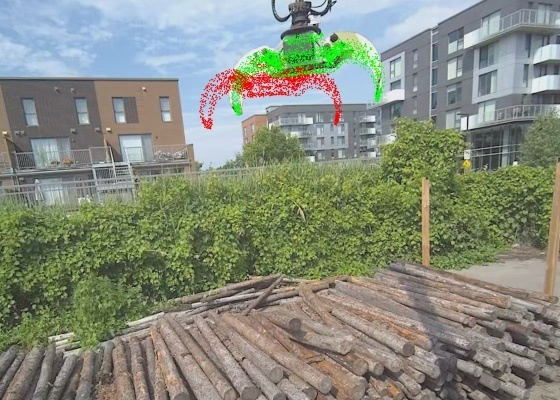
\includegraphics[width=\linewidth]{figures/calib/grapple_reproj_zed0.jpg}
\end{minipage}\hfill
\begin{minipage}{0.49\linewidth}
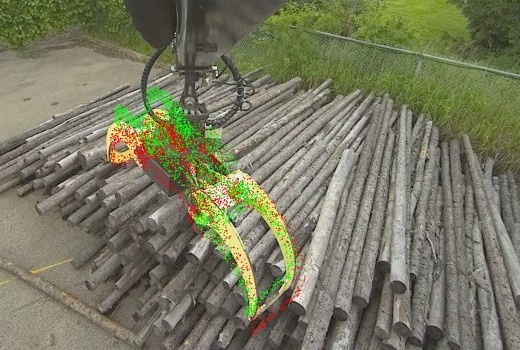
\includegraphics[width=\linewidth]{figures/calib/grapple_reproj_zed1.jpg}
\end{minipage}
\caption{Reprojection validation of the grapple-based calibration. The
grapple model, posed by forward kinematics and projected through the
floor-constrained calibrated mount (green) and through the nominal
uncalibrated mount (red), is overlaid on the mast camera (left) and stick
camera (right) images. In both views the calibrated model lands on the
observed grapple; the nominal mount is visibly displaced for the mast
camera, whose bracket pose is the one that changes whenever the mount is
adjusted.}
\label{fig:s2r_grapple_reproj}
\end{figure}

\begin{figure}[t]
\centering
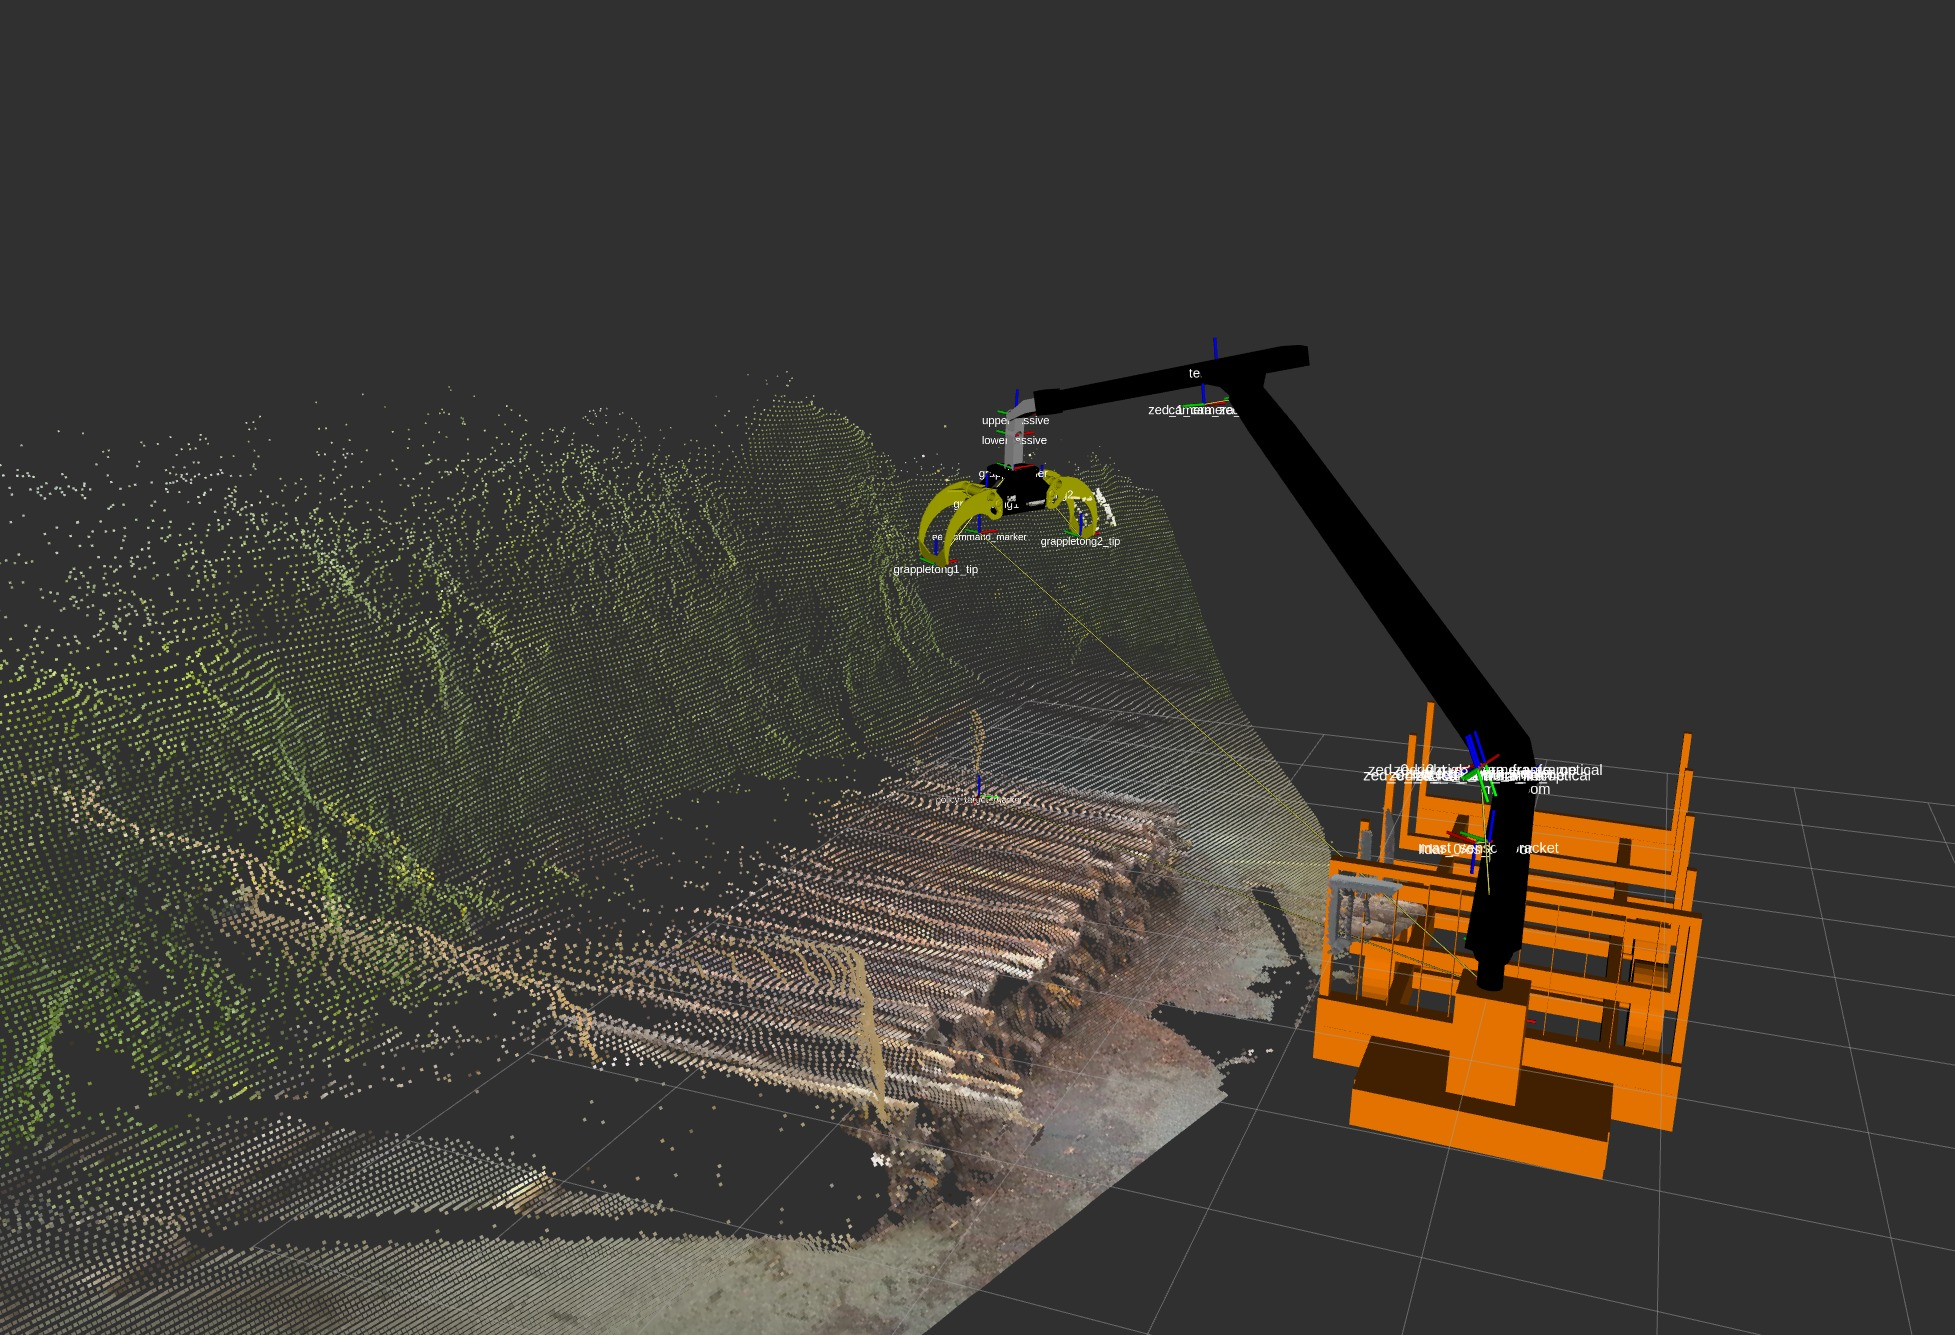
\includegraphics[width=0.92\linewidth]{figures/calib/replay_rviz.jpg}
\caption{Replay validation of the full calibration. Recorded camera and
joint-state data are replayed against the machine description carrying the
calibrated mounts, which is the sole transform authority: the crane model is
posed by the recorded joint states, and the registered camera cloud is
placed in the base frame through the calibrated extrinsics. The cloud lands
on the model consistently, with the observed pile, rack, and ground where
the model expects them.}
\label{fig:s2r_replay}
\end{figure}

\section{Rack Localization}
\label{sec:s2r_rack}

The action volume, the crop box, and the simulated rack must all sit where
the physical rack sits. The rack's 7.38~m length defeats single-camera
localization: no one viewpoint sees both ends with usable depth, so both
calibrated cameras are fused in the base frame. Printed fiducial
markers~\cite{garridojurado2014automatic} on the rack posts are detected in
full-resolution frames from each camera (Figure~\ref{fig:s2r_aruco}), each
detection lifted to the base frame through the camera's forward-kinematics
chain and calibrated mount. The mast camera contributes the near posts and
the stick camera the far post, and the marker pair spanning the rack's long
edge, a 7.5~m cross-camera baseline, fixes the rack yaw far more precisely
than any short edge. Because depth is the weak axis of fiducial pose
estimation at range (meter-scale errors at 7~m), marker detections only seed
the fit; the post columns visible in the registered point cloud refine the
corner positions, and the known rigid rack footprint ($2.16 \times 7.38$~m)
is fitted for pose only, anchored on the two reliable corner posts. The
recovered rack pose placed the rack bottom on the ground plane to within
24~mm of the simulator's, and reprojecting the fitted rack wireframe onto
the camera image shows the box edges following the physical posts
(Figure~\ref{fig:s2r_wireframe}). The procedure was re-run from a single
recorded sequence when the crane was later repositioned.

\begin{figure}[t]
\centering
\begin{minipage}{0.49\linewidth}
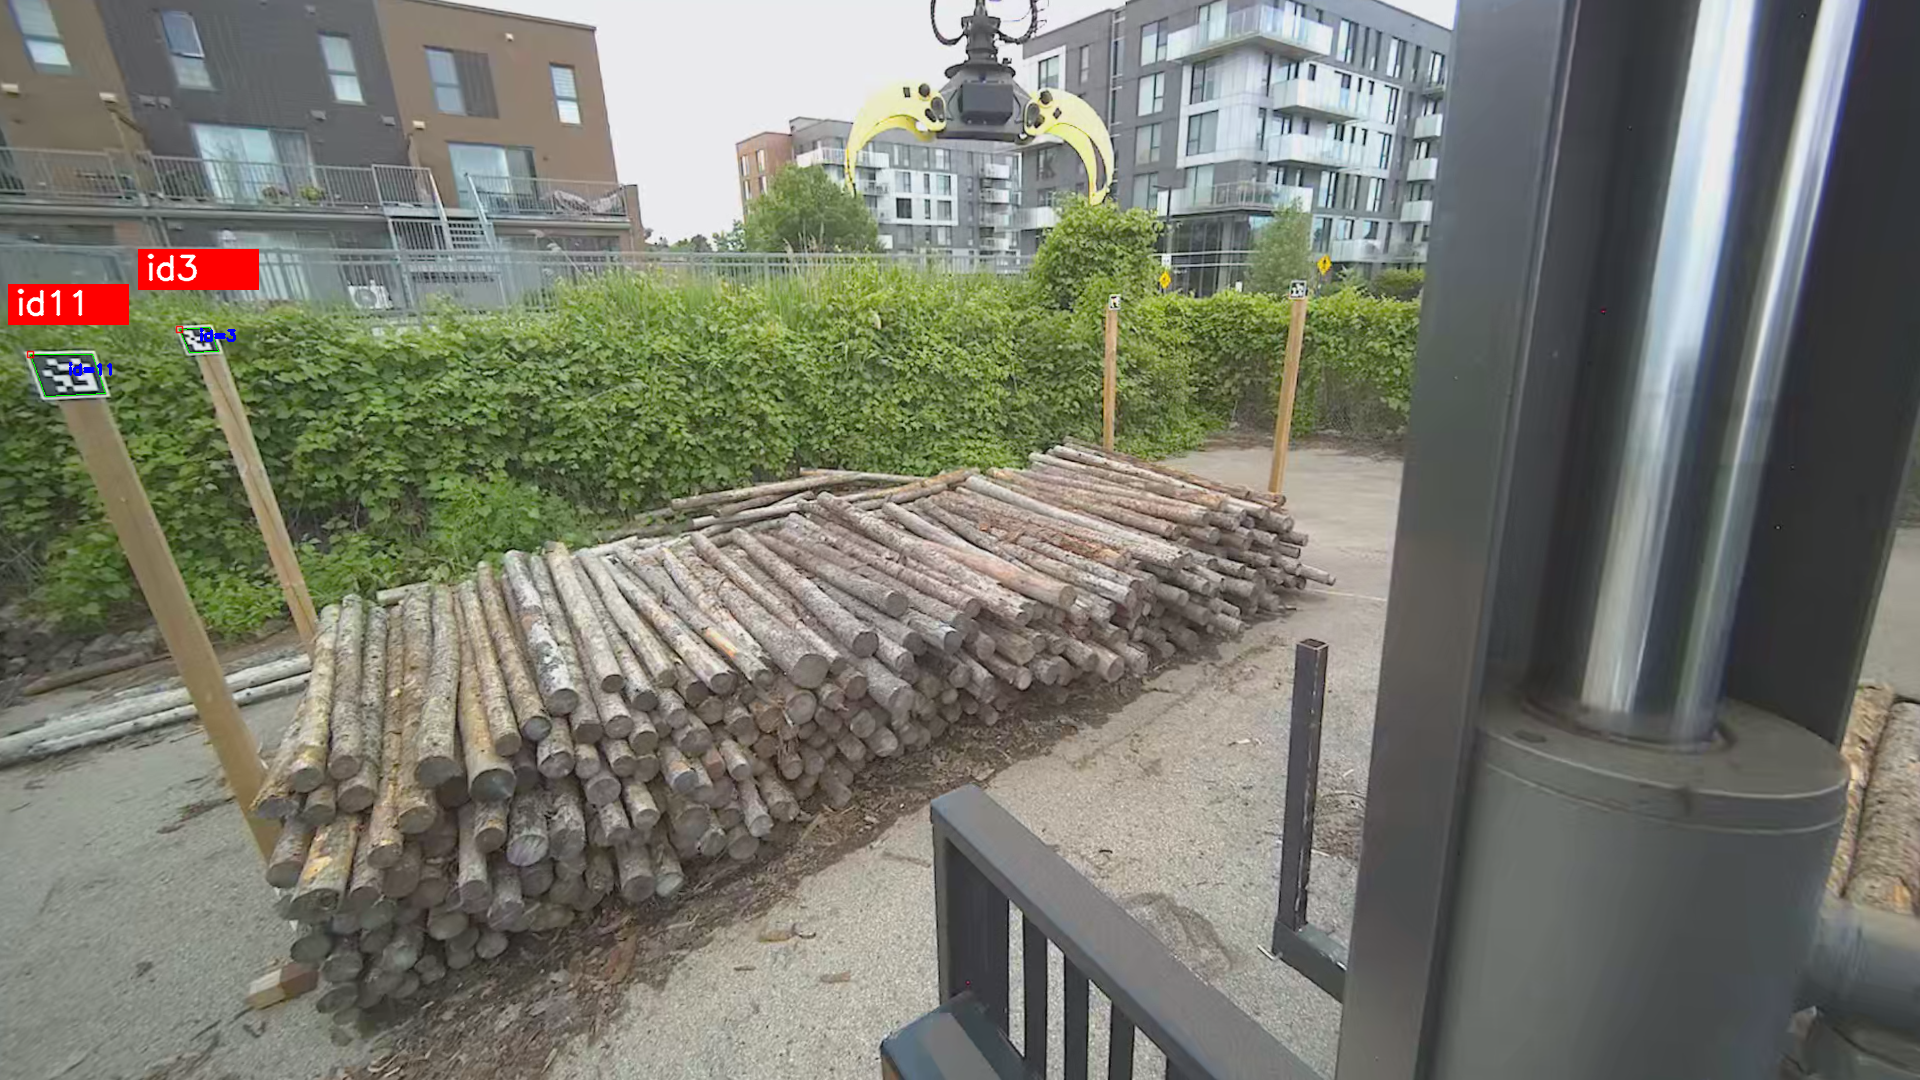
\includegraphics[width=\linewidth]{figures/calib/det_zed0.png}
\end{minipage}\hfill
\begin{minipage}{0.49\linewidth}
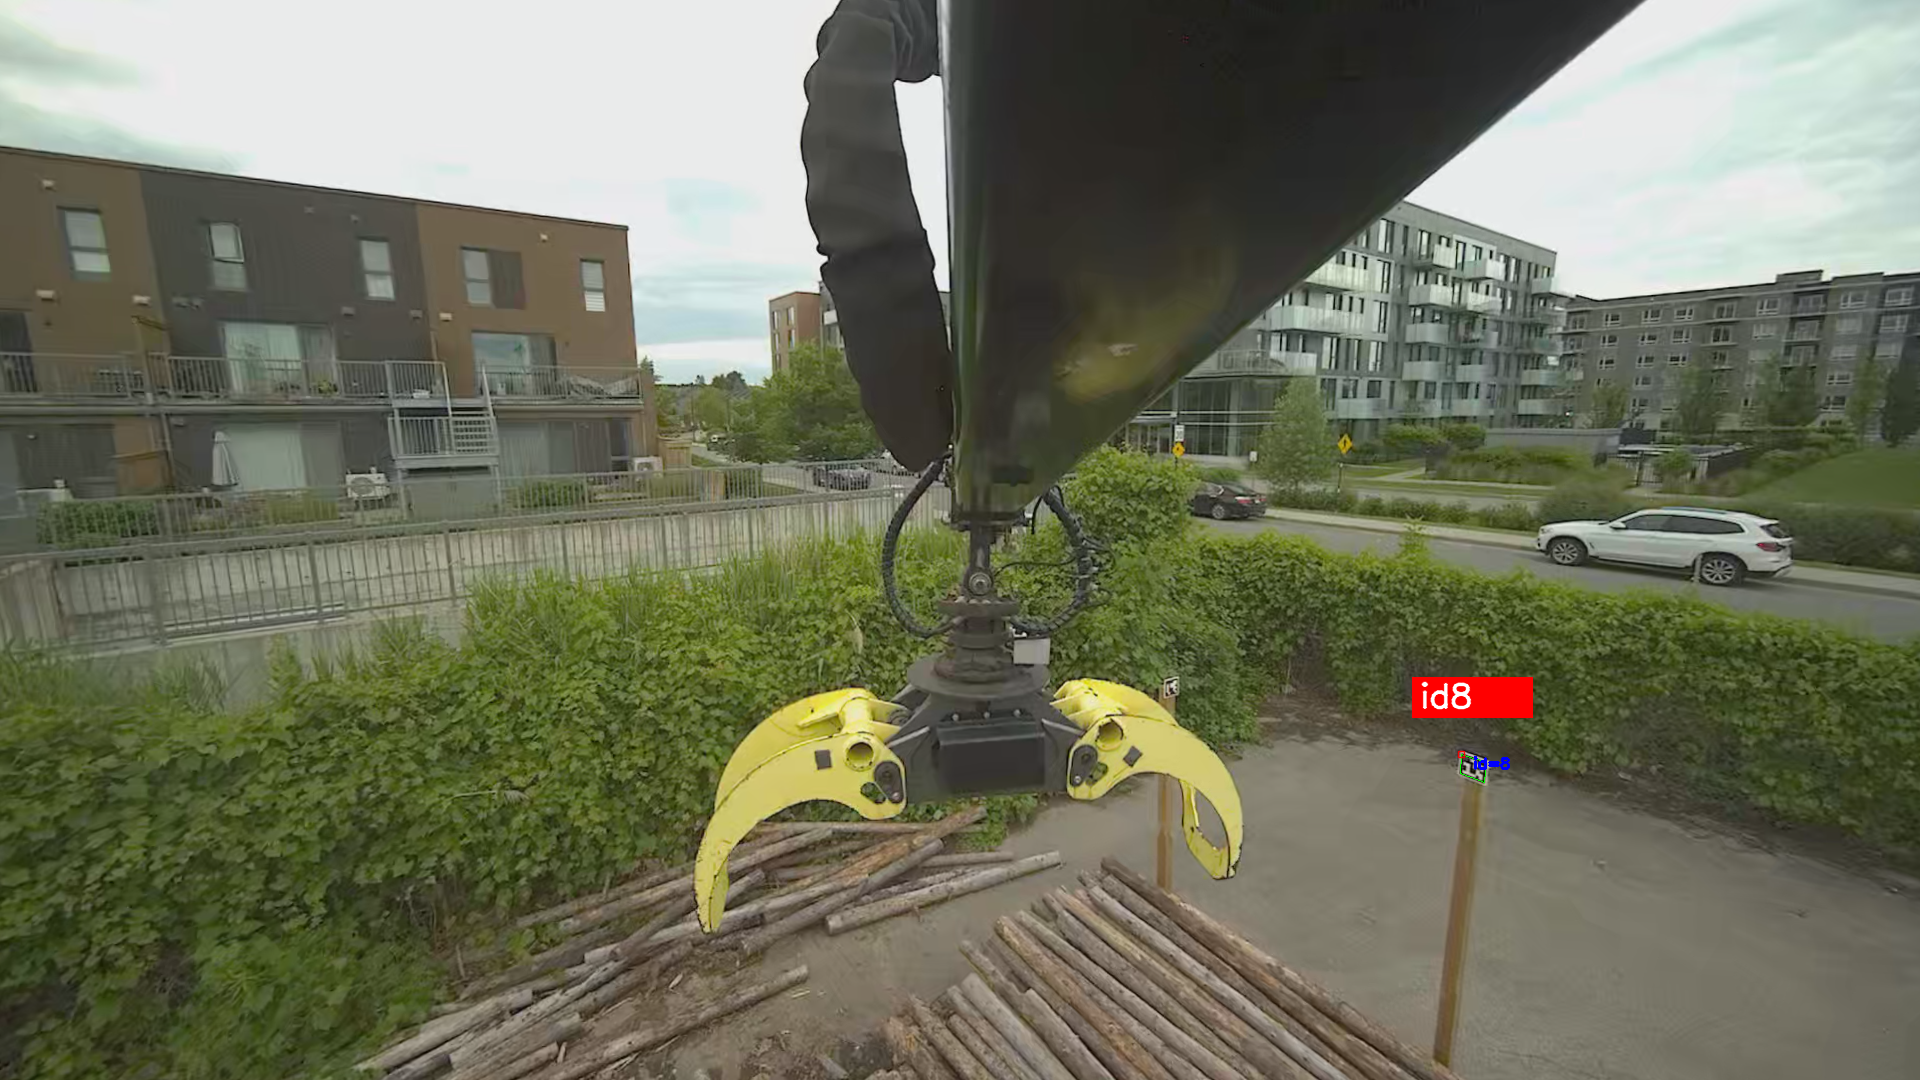
\includegraphics[width=\linewidth]{figures/calib/det_zed1.png}
\end{minipage}
\caption{Fiducial detections for rack localization. Left: the mast camera
sees the near rack posts. Right: the stick camera reaches the far post that
the mast camera cannot resolve, motivating the two-camera fusion.}
\label{fig:s2r_aruco}
\end{figure}

\begin{figure}[t]
\centering
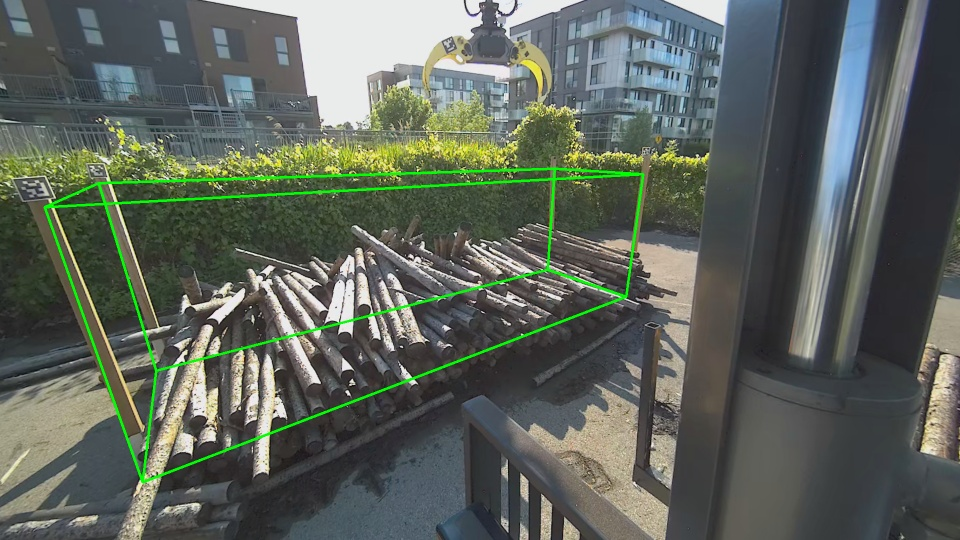
\includegraphics[width=0.8\linewidth]{figures/calib/rack_final_wire7.jpg}
\caption{Validation of the fused rack localization: the fitted rack box,
reprojected through the calibrated mast camera, follows the physical posts
and rails.}
\label{fig:s2r_wireframe}
\end{figure}

\section{Matching the Training Environment to Deployment}
\label{sec:s2r_gaze}

With mounts and rack calibrated, the simulation is updated so that the
training observation is generated the way the deployed observation will be.

\emph{Sensor and scene placement.} The calibrated camera mounts are baked
into the machine description used by both the deployed nodes and the
simulator, the simulated mast camera is attached to the mast link at the
calibrated transform, and the rack is placed at the calibrated base-frame
pose. The simulated camera's resolution and intrinsics are matched to the
calibrated ZED parameters.

\emph{The gaze phase.} On the real crane the mast camera's view depends on
the crane's configuration, and the arm can occlude the rack. The training
environment therefore adds a \texttt{GAZE} phase to the grasp cycle: before
each targeting decision the crane drives to a fixed joint-space gaze pose,
measured from recorded data of the physical crane parked in its viewing
configuration, in which the camera frames the rack and the arm is clear of
the view. The observation for each decision is captured at this pose, once
per cycle, exactly as at deployment. The environment step boundary is placed
at the settled gaze pose, so a policy step observes the gaze-pose cloud,
commands a grasp, and returns after the cycle completes and the crane is
back at gaze. This configuration, with the calibrated long rack and piles of
approximately 200 logs, is the training environment for all deployment-bound
policies in Chapters~\ref{ch:bc_policies} and \ref{ch:bcrl}.

\emph{Verification.} Figure~\ref{fig:s2r_gaze_rgb} compares the real and
simulated camera views at the gaze pose, and Figure~\ref{fig:s2r_overlay}
overlays simulated and real point clouds in the base frame. With calibrated
extrinsics the clouds land on the same rack volume, sharing the rack-region
extent in both horizontal axes. The residual differences are exactly the
sensor-realism gaps: real stereo depth carries holes and range-dependent
noise where simulated depth is complete and clean, and the real floor sits
about 13~cm below the simulated one. These observations motivate the
range-dependent noise augmentation of
Chapter~\ref{ch:bc_policies} and the observation crop, which
removes the floor from the policy input in both domains.

\begin{figure}[t]
\centering
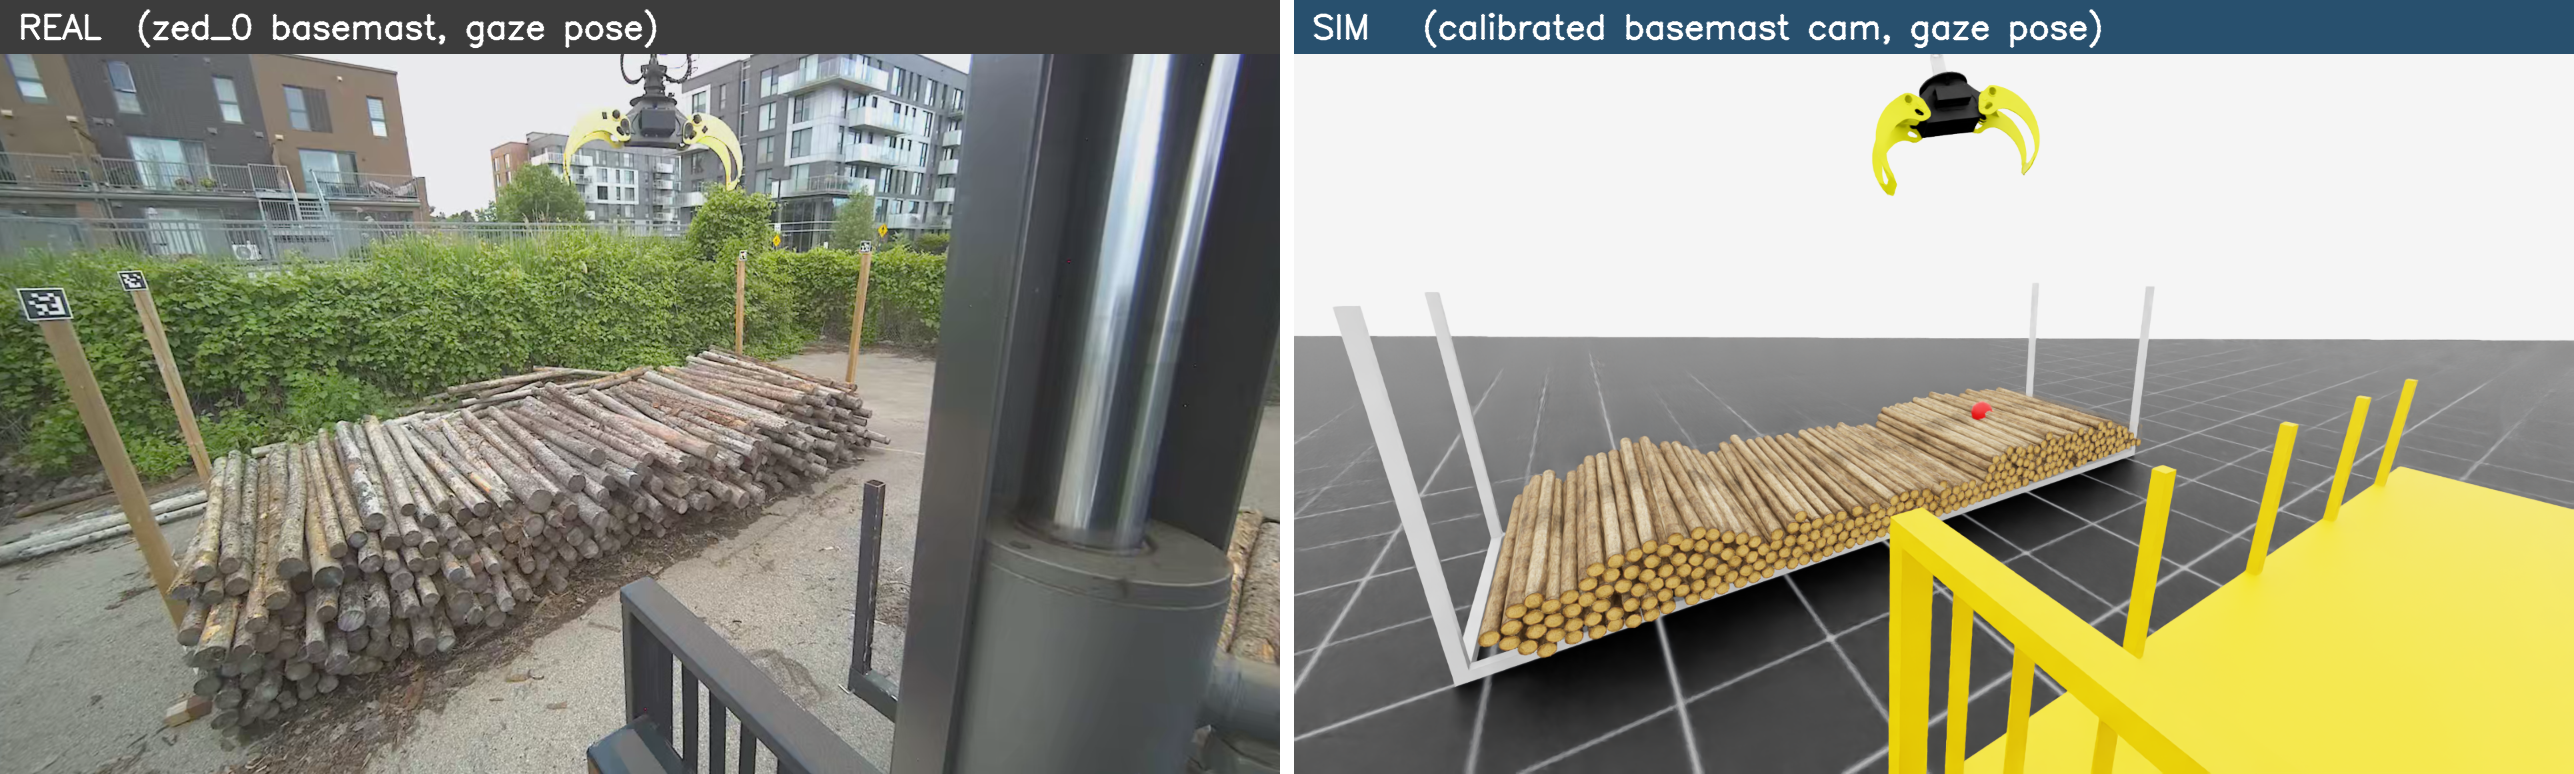
\includegraphics[width=\linewidth]{figures/calib/gaze_real_vs_sim.png}
\caption{Real (left) and simulated (right) mast-camera views at the gaze
pose after calibration. The simulated camera reproduces the deployed
viewpoint: grapple top-center, pile and rack in the lower half, matching
framing of the workspace.}
\label{fig:s2r_gaze_rgb}
\end{figure}

\begin{figure}[t]
\centering
\begin{minipage}{0.51\linewidth}
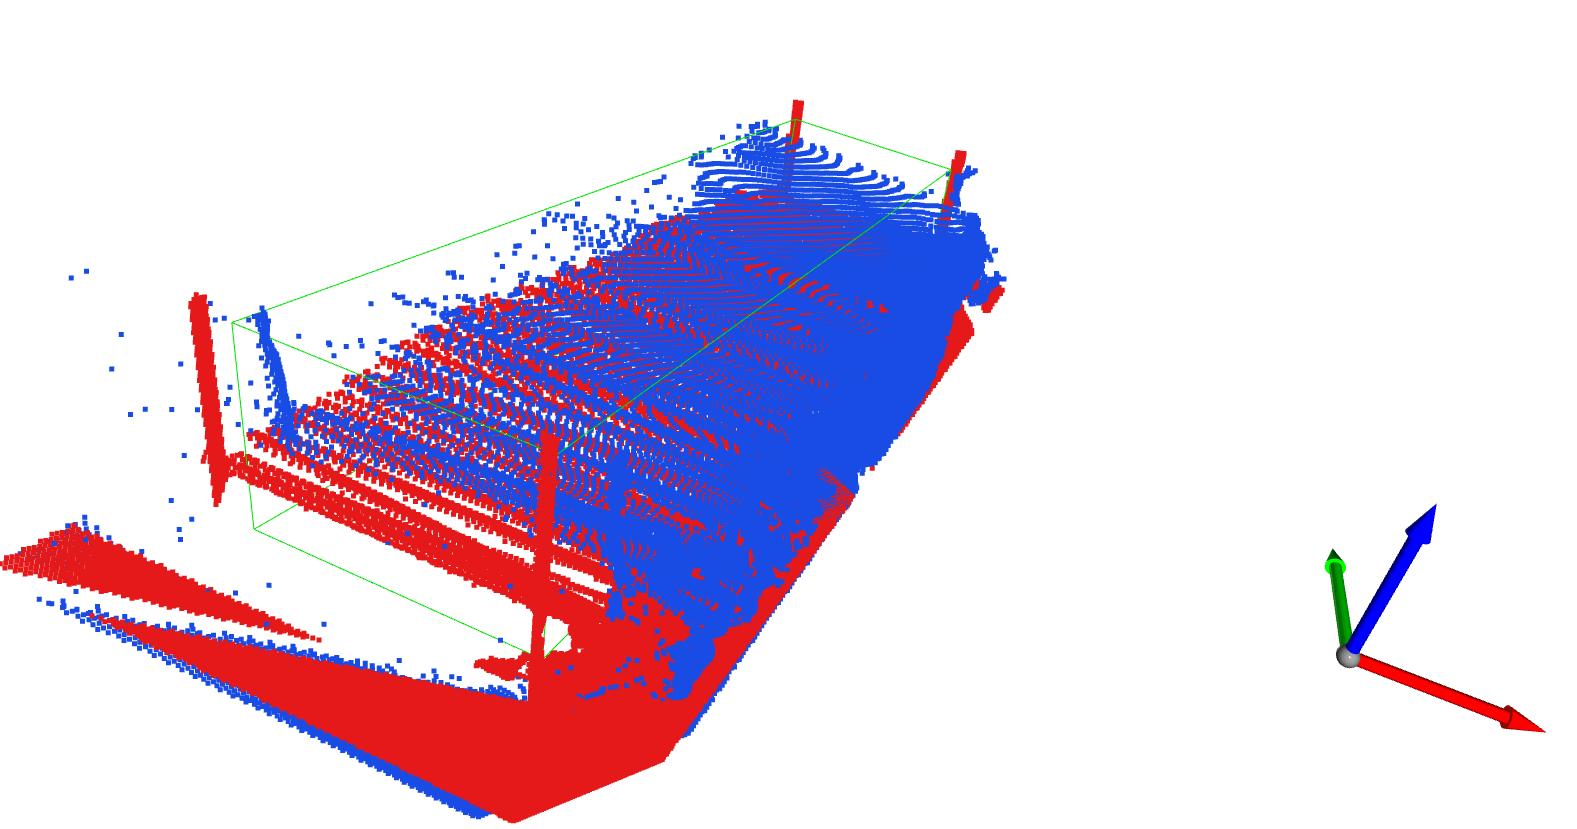
\includegraphics[width=\linewidth]{figures/calib/pcd_overlay_iso.png}
\end{minipage}\hfill
\begin{minipage}{0.47\linewidth}
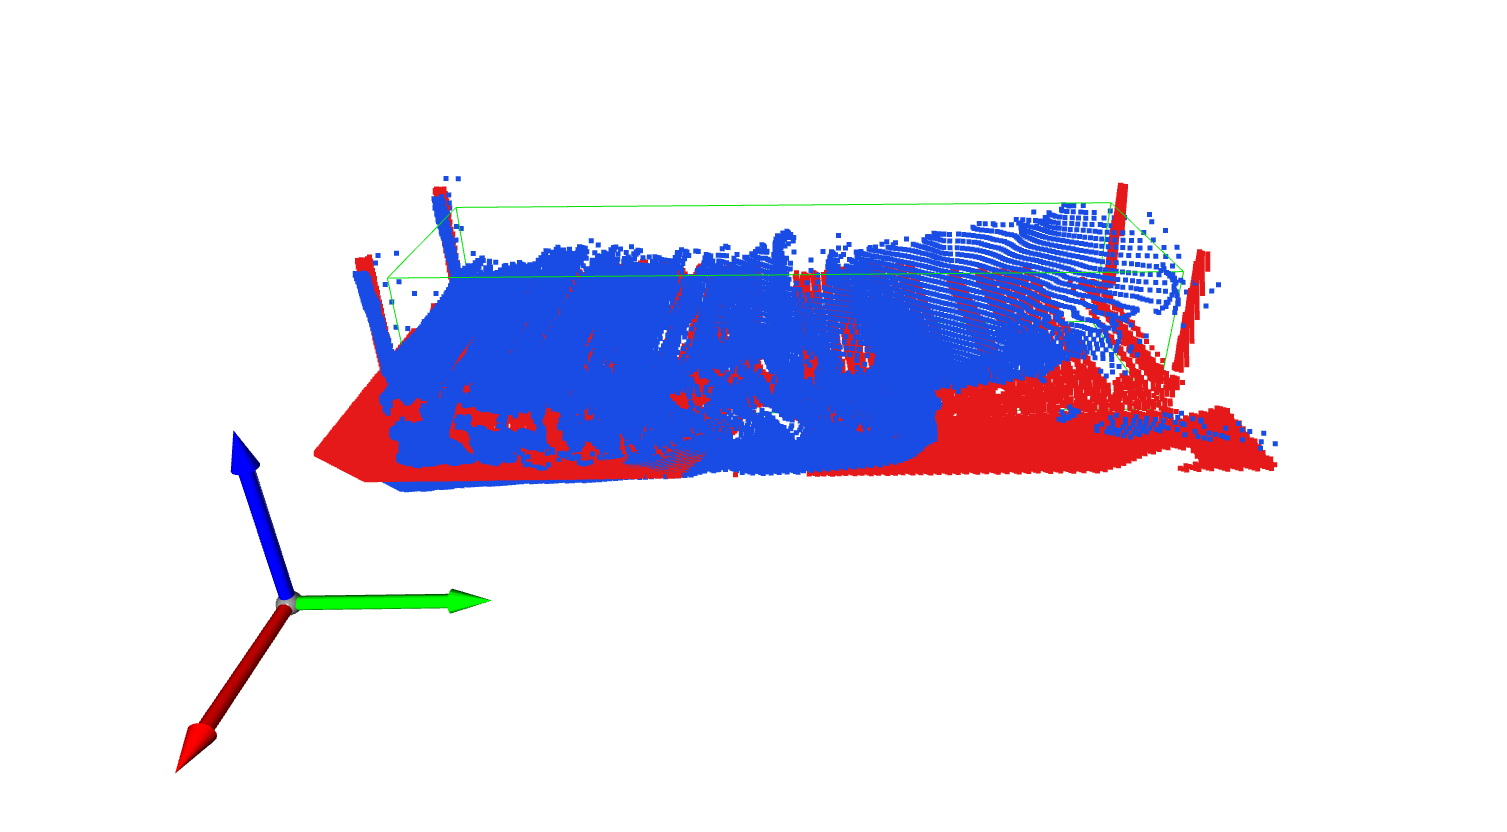
\includegraphics[width=\linewidth]{figures/calib/pcd_overlay.png}
\end{minipage}
\caption{Simulated (red) and real (blue) point clouds overlaid in the crane
base frame with the action volume in green; isometric (left) and side
(right) views. Calibration places both clouds on the same rack volume; the
remaining discrepancies are stereo holes and noise in the real cloud and a
floor-height offset of roughly 13~cm, both handled in the observation
pipeline.}
\label{fig:s2r_overlay}
\end{figure}

\section{Deposition}
\label{sec:s2r_deposit}

The learned decision ends at target selection; what happens to a grasped
bundle is sequenced by engineered logic in the policy node. After a
successful lift the crane carries the bundle to its home configuration and
deposits it into the trailer-bed area beside the rack, and the deposition
logic decides where along the trailer and from what height each bundle is
released.

The deposit area is divided into compartments by divider poles whose
positions were measured on the platform, giving four bins of roughly 1.28~m
width along the trailer axis. Bundles are laid across the active bin, with
the grapple yaw held perpendicular to the trailer length, and the bins are
filled in rotation from the far end toward the crane, one bundle per bin per
pass, so the load builds up in even layers; the bin nearest the crane is
excluded because the arm cannot load it cleanly. A bin counts as full once
its scanned fill height reaches a threshold, and when the last bin fills,
the run ends.

The release height adapts to the fill state
(Figure~\ref{fig:s2r_deposit}). Before each drop, with the crane settled at
the home pose, the mast-camera cloud is scanned over the active bin only,
inset from the divider poles so they are not mistaken for cargo, and the
release height is set a fixed clearance above the detected fill top. The
scan is gated for freshness the same way the gaze observation is: its sensor
timestamp must postdate the settling of the crane, so the held bundle and
the swinging grapple cannot inflate the measured fill height. A bin the
camera cannot yet see into falls back to a conservative blind release
height, and the first drop into an empty bin descends lower so the bundle
does not scatter. The per-bin fill state persists to disk, so an
interrupted run resumes its fill sequence instead of restarting it. All
field trials of Chapter~\ref{ch:bc_policies} run with this deposition
pipeline; a cycle succeeds only if it deposits at least one log, so
deposition is part of the measured system.

\begin{figure}[t]
\centering
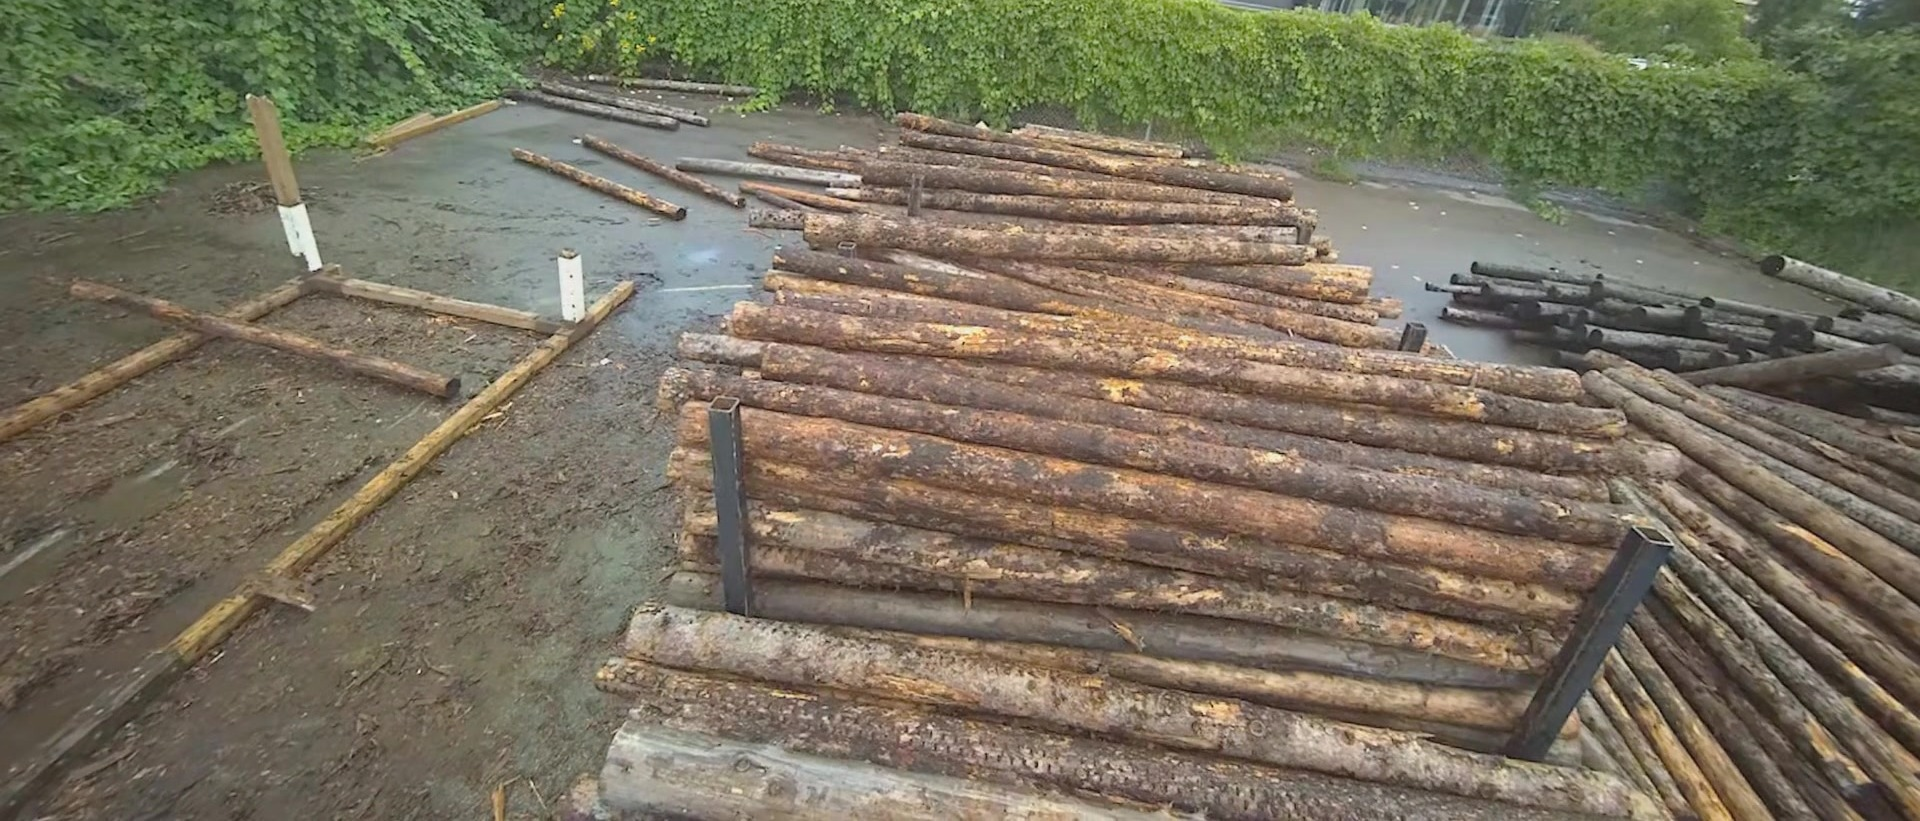
\includegraphics[width=0.9\linewidth]{figures/deposit_bins_photo.jpg}

\vspace{2mm}
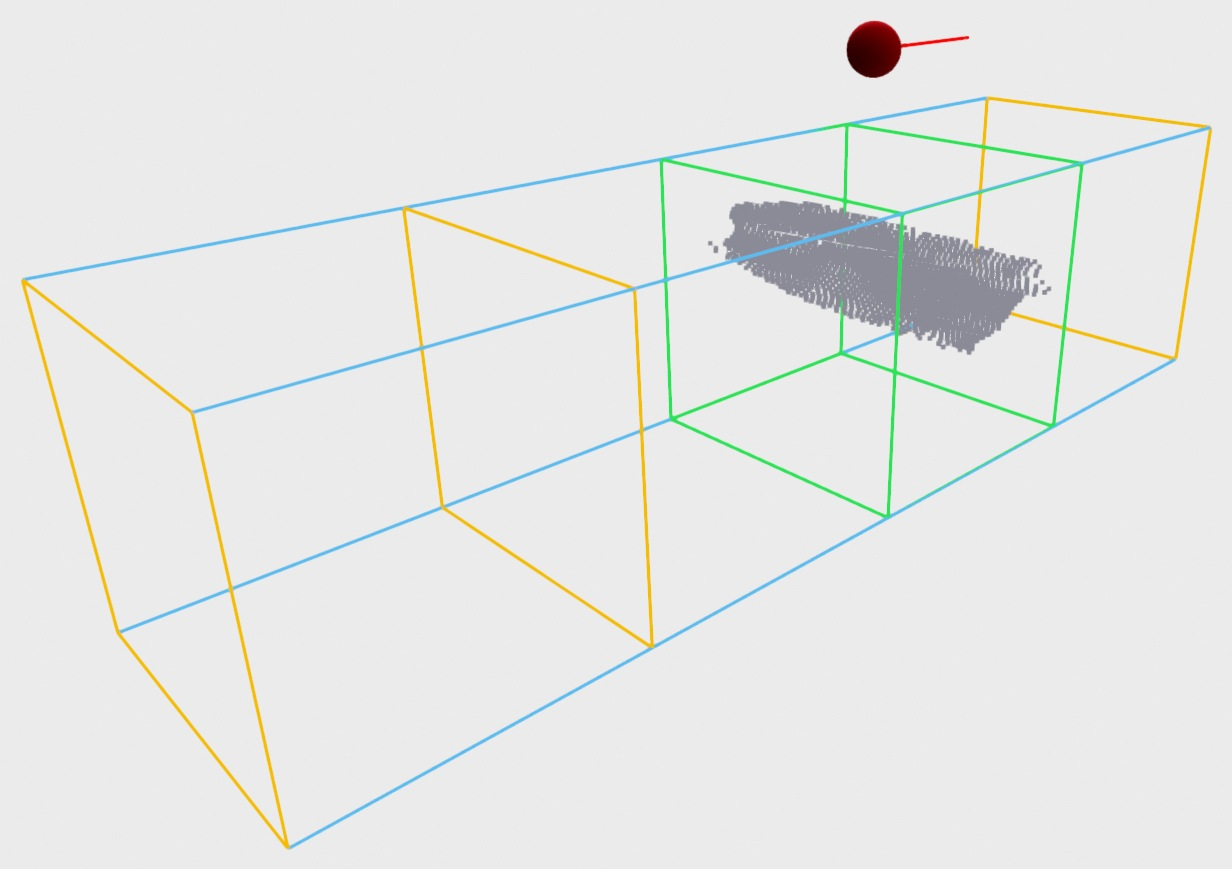
\includegraphics[width=0.88\linewidth]{figures/deposit_bin_iso.jpg}
\caption{Bin deposition during a field trial. Top: the mast-camera capture
this cycle's deposit scan was computed from, taken with the crane settled at
the home pose just before lowering to release; earlier bundles lie across
the pole-divided compartments beyond the rack, and the remaining pile is in
the foreground. Bottom: the deposit scan derived from that capture, in the
crane base frame. The deposit volume (blue) is split by the measured
divider planes (orange); only points inside the active compartment (green)
are retained (gray), and the release target (red sphere, with the commanded
grapple yaw as the red line) is placed a fixed clearance above their
detected top.}
\label{fig:s2r_deposit}
\end{figure}

\section{Deployment Pipeline Safeguards}
\label{sec:s2r_deploy}

Four further elements of the deployed pipeline matter for the field results
of Chapter~\ref{ch:bc_policies}.

\emph{Identical observation processing.} The deployed policy node runs
Algorithm~\ref{alg:obs_pipeline} unchanged: base-frame transform with the
calibrated extrinsics of Section~\ref{sec:s2r_camcalib}, crop to the
calibrated box, farthest point sampling to the trained budget, zero padding.
The decode that follows is Algorithm~\ref{alg:scoring_decode}, again
unchanged, with the action box supplied as a runtime parameter. Any deviation
between the two pipelines is a distribution shift the policy pays for
directly.

\emph{Actuation envelope.} Commanded grasp heights are clamped to the
platform bed level plus a safety margin at a single choke point, applied
identically to every target source (learned policies and the heuristic
baseline) and mirrored in the simulator's action decode. The commanded
height is the grasp center and the grapple tines sweep below it, hence the
margin; the clamp trades access to the bottom log layer for jam safety, a
platform constraint documented with the trials.

\emph{Frame recalibration.} The policies are trained in a fixed base-frame
coordinate system, and Chapter~\ref{ch:bc_policies} shows they are not
robust to translations of the scene within that frame. When the physical
rack was found to have shifted 0.45~m along the rack axis from its
calibrated position, the correction was a measured offset parameter that
translates the crop box onto the rack, returns the cropped cloud to training
coordinates for the network, and adds the offset back to the decoded
command. Scene geometry is thus treated as a calibrated quantity with a
defined recalibration procedure, not something the policy is expected to
absorb.

\emph{Run instrumentation.} Every deployed run writes a synchronized
record: a per-cycle dump of the policy input cloud and decoded target
(Figure~\ref{fig:s2r_policy_debug}), the deposit scan of each drop
(Figure~\ref{fig:s2r_deposit}), and decision and phase logs that index every
decision to the exact frame of the recorded camera stream. Any decision in a
trial can therefore be audited offline against exactly what the policy saw,
which is what makes the failure analysis and the offline policy replays of
Chapter~\ref{ch:bc_policies} possible.

\begin{figure}[t]
\centering
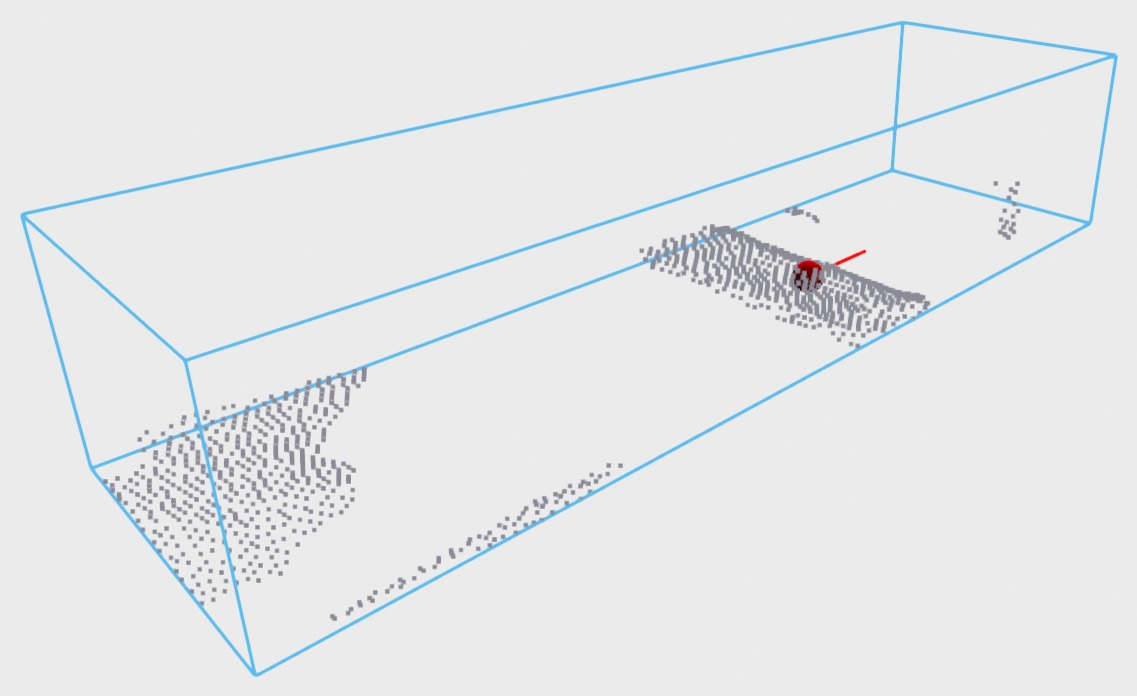
\includegraphics[width=0.85\linewidth]{figures/policy_debug_iso.jpg}
\caption{Per-cycle decision record from a field trial: the policy input
cloud (gray) inside the action volume (blue), with the decoded grasp target
(red sphere) and commanded yaw (red line), dumped at the moment of the
decision. This record is from the same cycle as the deposit scan of
Figure~\ref{fig:s2r_deposit}, late in the trial, when the policy targets
the last remaining row of logs.}
\label{fig:s2r_policy_debug}
\end{figure}

\section{Summary}

The transfer infrastructure rests on three measured results: the control
chain tracks commanded grasp targets to 1.5~cm over the rack workspace; the
grapple-based, floor-constrained calibration places both cameras' clouds in
the base frame with decimeter-scale registration residuals and ground-plane
tilt at the tenth-of-a-degree level; and the fused rack localization agrees
with the simulator's scene to centimeters, validated by wireframe
reprojection. On top of these, the training environment reproduces the
deployed viewpoint through the calibrated camera mount, the measured gaze
pose, and the calibrated rack placement, and the deployed pipeline
reproduces the training observation processing exactly. What remains between
simulation and the crane is the sensor-realism gap (stereo noise and holes)
and the behavioral consequences of pile geometry, which are the subject of
the next chapter.

% Thesis chapter: training the regression and scoring BC policies, and their differences.
% Standalone chapter file; \input or \include from the thesis root.
% Requires graphicx; figures live in figures/ relative to this file.
% Sources: scripts/envs/train_bc_pointcloud.py (regression),
%          scripts/envs/scoring_head.py + train_scoring_head.py (scoring),
%          scripts/envs/summarize_noise_sweep.py (degradation sweep),
%          real_trials.ods + render_policy_comparison.py (field trials).

\chapter[Learning Grasp Selection from Point Clouds]{Learning Grasp Selection from Point Clouds: Regression and Scoring Policies}
\label{ch:bc_policies}

This chapter describes the two behavior-cloned grasp policies used on the crane:
a \emph{regression} policy that maps the observed point cloud directly to grasp
coordinates, and a \emph{scoring} policy that scores every observed point and
grasps at the highest-scoring one. Both are trained by supervised learning on
the same expert demonstrations and share the same PointNet feature trunk; they
differ only in how the grasp is parameterized and, consequently, in the loss
that supervises it. That difference determines their behavior: the regression
policy minimizes a mean-squared error and therefore averages over multimodal
expert behavior, while the scoring policy minimizes a classification loss over
observed points and is mode-seeking by construction. Section~\ref{sec:bc_common}
covers the shared data pipeline, Sections~\ref{sec:bc_regression} and
\ref{sec:bc_scoring} the two policies, and Section~\ref{sec:bc_differences}
makes the differences explicit. Section~\ref{sec:bc_trials} closes the loop
with field trials on the physical crane: a three-trial baseline campaign whose
failure analysis motivated the scoring design, offline replays of both
policies on the recorded failure clouds, a simulated observation-degradation
sweep, and two hardware trials of the scoring policy itself.

\section{Common Setup: Demonstrations, Observations, and Labels}
\label{sec:bc_common}

\subsection{Expert demonstrations}

Demonstrations are collected in simulation from a privileged expert that reads
ground-truth log poses. At each grasp cycle the expert selects the topmost log
in the rack, targets its center, and computes the grapple yaw that aligns the
grapple with the log's long axis. Executing this expert clears piles reliably,
so the dataset records one tuple per successful grasp cycle:
\begin{equation}
  \mathcal{D} = \big\{ (P_k,\; t_k,\; \psi_k) \big\}_{k=1}^{M},
\end{equation}
where $M$ is the number of recorded cycles,
$P_k \in \mathbb{R}^{N \times 3}$ is the point cloud observed at the
start of the cycle, $t_k = (t_x, t_y, t_z) \in \mathbb{R}^3$ is the commanded
grasp center in the crane base frame, and $\psi_k$ is the commanded grapple
yaw. Because the expert targets log \emph{centers}, the label height satisfies
$t_z = z_{\mathrm{surf}} - r_{\log}$ by construction, where
$z_{\mathrm{surf}}$ is the local pile surface and $r_{\log} = 0.056$~m is the
log radius. This identity is what later allows relabeling to a different
digging depth (Section~\ref{sec:bc_dig}).

Piles are randomized between episodes. The final collection recipe spawns
profiled piles (localized mounds with randomized amplitude, width, and
multi-bump structure, plus per-log scale jitter) and truncates episodes after a
small number of grasp cycles so that mound-shaped, informative states dominate
the dataset rather than the flat late-episode remainders.

\subsection{Observation pipeline}

The observation is a simulated depth-camera point cloud processed by
Algorithm~\ref{alg:obs_pipeline}, the same procedure the deployed node runs.
The raw camera cloud is transformed into the crane
base frame, cropped to an axis-aligned box around the rack, and downsampled
with farthest-point sampling (FPS) to a fixed budget of $N$ points ($N = 1024$
for the tight-crop datasets, $N = 2048$ for the widened-crop datasets):
\begin{equation}
  P = \mathrm{FPS}_N\!\left( \mathrm{crop}_{[b^{\min} - m,\; b^{\max} + m]}
      \left( T_{\mathrm{base} \leftarrow \mathrm{cam}} \, P_{\mathrm{raw}} \right) \right).
\end{equation}
Here $[b^{\min}, b^{\max}]$ is the action box, the volume of commandable grasp
centers,
\begin{equation}
  b^{\min} = (-5.364,\; -1.684,\; -1.30), \qquad
  b^{\max} = (-3.364,\; 5.316,\; 0.10) \quad [\mathrm{m}],
\end{equation}
and $m$ is an optional crop margin. The tight datasets use $m = 0$ (the
observation crop equals the action box); the margin datasets use $m = 0.5$~m
in $x$ and $y$, so the policy also sees context immediately outside the box
(bed apron, rack posts) while the set of commandable grasps is unchanged.
Clouds with fewer than $N$ points after cropping are zero-padded, and both
policies mask padded slots explicitly.

The margin exists because of a sim-to-real asymmetry, illustrated in
Figure~\ref{fig:bc_sim_vs_real_crop}. In simulation the tight crop removes
the bed plane, the rack rails, and the pole columns, so a tight-crop policy
trains on clouds that contain logs and nothing else. On the real crane those
surfaces intrude into the same crop volume: rack ends, pole columns, and the
bed remain visible, and late in a trial, once the pile drops below the rail
height, they become the most prominent geometry in the crop. A policy trained
on the tight crop therefore never sees, at training time, the structure it is
most likely to mis-target at deployment. Widening the observation crop and
spawning the corresponding structure in simulation restores parity between
what the network trains on and what it will be shown.

\begin{figure}[t]
\centering
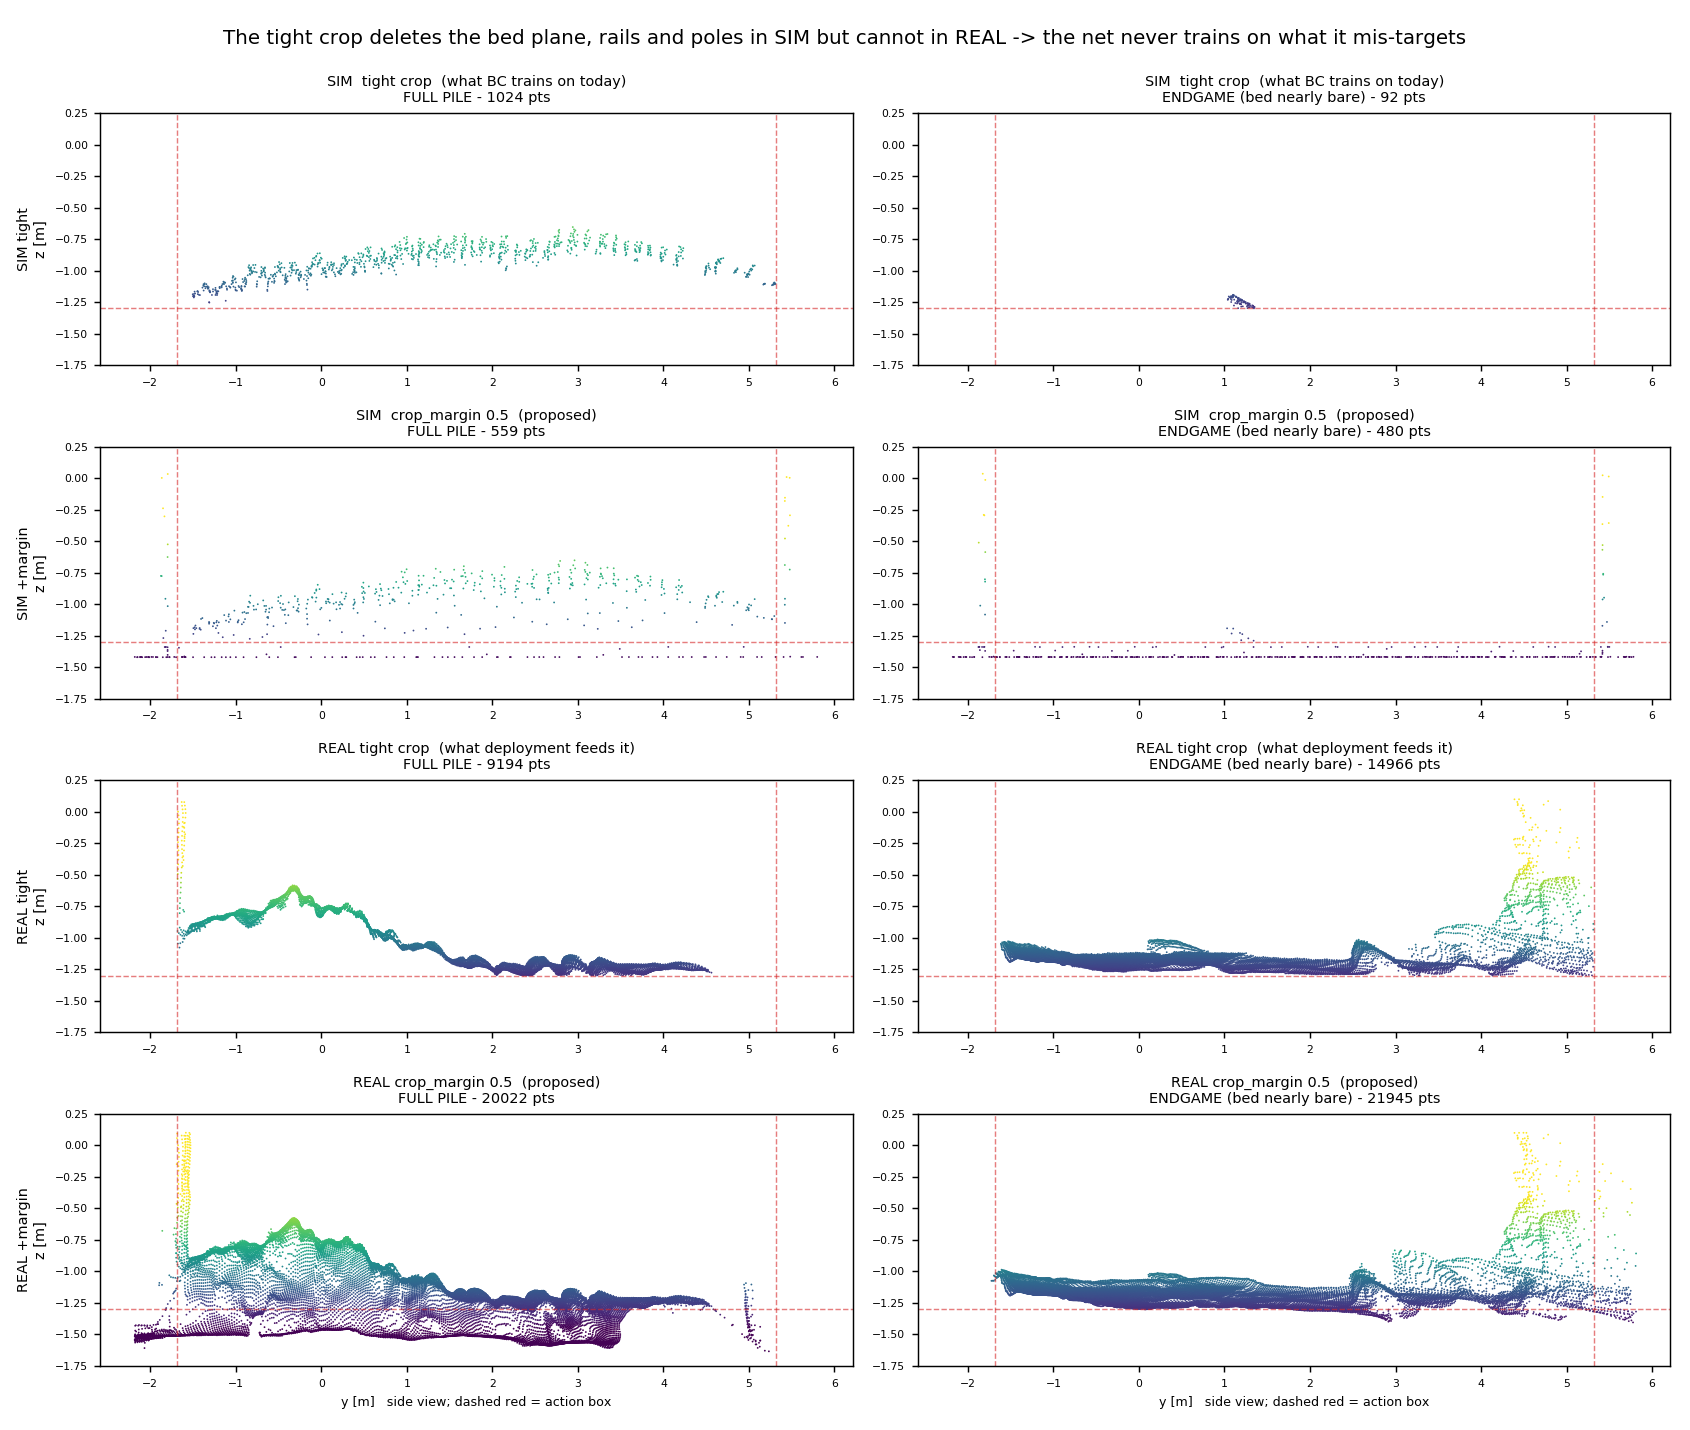
\includegraphics[width=\linewidth]{figures/sim_vs_real_crop.png}
\caption{Side views ($y$--$z$) of simulated and real clouds under the tight
crop and the widened ($m = 0.5$~m) crop, for a full pile (left column) and a
late-trial state (right column); dashed red lines mark the action box. The
tight crop deletes the bed plane, rails, and poles in simulation but cannot
do so on the real crane, where they dominate the late-trial cloud. The
margin crop makes the training observation contain the same structure classes
as the deployment observation.}
\label{fig:bc_sim_vs_real_crop}
\end{figure}

\subsection{Sensor noise model}
\label{sec:bc_noise}

Clouds are collected clean and corrupted with fresh noise at every training
epoch, using an axial noise model fitted to the real ZED stereo camera. Each
point is displaced along its camera ray with a standard deviation that grows
quadratically with range:
\begin{equation}
  \tilde{p}_i = p_i + \eta_i \, \frac{p_i - c}{\lVert p_i - c \rVert}, \qquad
  \eta_i \sim \mathcal{N}\!\left(0,\; \sigma^2(r_i)\right), \qquad
  \sigma(r_i) = \nu \, r_i^2,
\end{equation}
where $c$ is the camera position in the base frame (stored with each dataset),
$r_i = \lVert p_i - c \rVert$, and $\nu = 0.0014$~m$^{-1}$. Padded slots
are left untouched. Applying the noise per epoch rather than at collection
time means every pass over the data sees a different corruption, which
regularizes both policies at no additional collection cost.

\section{The Regression Policy}
\label{sec:bc_regression}

\subsection{Action parameterization}
\label{sec:bc_action_param}

The regression policy outputs a five-dimensional action
$a = (a_x, a_y, a_z, a_c, a_s)$ that encodes the grasp center and yaw. The
three position components are encoded by normalizing the metric target to the
action box and applying the inverse hyperbolic tangent,
\begin{equation}
  u_j = \mathrm{clip}\!\left( \frac{2\,(t_j - b^{\min}_j)}{b^{\max}_j - b^{\min}_j} - 1,\;
        -0.999,\; 0.999 \right), \qquad
  a_j = \operatorname{artanh}(u_j), \qquad j \in \{x, y, z\},
  \label{eq:arctanh_enc}
\end{equation}
so that at deployment the unbounded network output decodes to a target that is
guaranteed to lie inside the box:
\begin{equation}
  \hat{t}_j = b^{\min}_j + \frac{\tanh(\hat{a}_j) + 1}{2}
              \left( b^{\max}_j - b^{\min}_j \right).
  \label{eq:arctanh_dec}
\end{equation}

Yaw is encoded as the cosine and sine of the \emph{doubled} angle,
\begin{equation}
  a_c = \cos 2\psi, \qquad a_s = \sin 2\psi, \qquad
  \hat{\psi} = \tfrac{1}{2} \operatorname{atan2}(\hat{a}_s, \hat{a}_c).
  \label{eq:yaw_enc}
\end{equation}
Doubling the angle folds the grapple's $\pi$-symmetry into the encoding: a
grasp at yaw $\psi$ and one at $\psi + \pi$ are physically identical, and
under Equation~\eqref{eq:yaw_enc} they map to the same label. This is not a
refinement but a requirement. With yaw encoded as a single scalar the expert
labels are contradictory (the same pile state can carry labels $\psi$ and
$\psi + \pi$), the regression cannot converge, and validation error plateaus
an order of magnitude higher; switching to the doubled cosine/sine encoding on
identical data reduced validation error by roughly a factor of nine.

\subsection{Architecture}

The policy is a PointNet encoder followed by a small fully connected actor
head. The encoder applies a shared per-point multilayer perceptron (MLP) to
every point and pools with a channelwise maximum, which makes the network
invariant to point ordering:
\begin{equation}
  h_i = \phi(p_i) \in \mathbb{R}^{256}, \qquad
  g = \rho\!\left( \max_{i = 1, \dots, N} h_i \right) \in \mathbb{R}^{256},
  \label{eq:pointnet}
\end{equation}
where $\phi$ is the per-point MLP $3 \to 64 \to 128 \to 256$ (linear layers
with batch normalization and ELU activations), the maximum is taken per
channel over all points, and $\rho$ is a linear projection $256 \to 256$ with
batch normalization and ELU. The actor head maps the global feature to the
action through dropout ($p = 0.2$) and an MLP $256 \to 128 \to 64 \to 5$ with
ELU activations:
\begin{equation}
  \hat{a} = \mathrm{MLP}_{\mathrm{actor}}\!\left( \mathrm{drop}(g) \right).
\end{equation}
The head dimensions deliberately match the actor of the reinforcement-learning
policies so that behavior-cloned weights load directly into the actor-critic
used for BC-to-RL fine-tuning.

\subsection{Training objective and optimization}

Training minimizes the mean-squared error between predicted and encoded expert
actions over the dataset:
\begin{equation}
  \mathcal{L}_{\mathrm{reg}}(\theta) =
  \frac{1}{|\mathcal{B}|} \sum_{k \in \mathcal{B}}
  \left\lVert \pi_\theta(P_k) - a_k \right\rVert_2^2 .
  \label{eq:mse}
\end{equation}
The optimizer is AdamW with learning rate $10^{-4}$ and weight decay
$10^{-4}$, batch size 64, gradient-norm clipping at 1.0, an
85\,/\,15 train\,/\,validation split, a reduce-on-plateau schedule (factor
0.5, patience 10 epochs), early stopping after 30 epochs without validation
improvement, and checkpointing of the best-validation-loss weights. The
per-epoch ZED noise of Section~\ref{sec:bc_noise} is applied to every training
batch; validation runs on clean clouds.

\subsection{Digging-depth relabeling and the label-clamping problem}
\label{sec:bc_dig}

The sim expert grasps at the log center, $0.056$~m below the local surface.
Real grapple close mechanics need a deeper bite: executed real grasps sit
$0.2$--$0.4$~m below the surface, and a hardware probe with the sim convention
raked across the pile without closing. The dataset is therefore relabeled to a
deployment digging depth $d$ by exploiting the identity
$t_z = z_{\mathrm{surf}} - r_{\log}$:
\begin{equation}
  t_z' = \max\!\left( t_z + r_{\log} - d,\; z_{\mathrm{floor}} \right),
  \label{eq:dig}
\end{equation}
where $z_{\mathrm{floor}}$ is the platform bed floor plus a safety margin
(the executable envelope). Only the label changes; the expert's executed
trajectories, and hence the collected cloud distribution, are untouched.

The clamp in Equation~\eqref{eq:dig} creates a problem specific to the
regression parameterization. With $d = 0.25$~m a large fraction of labels hit
the floor, so the $z$ label distribution is flattened toward a constant and
the regression target loses much of its dependence on the input; the effect
is visible directly in the relabeled dataset
(Figure~\ref{fig:bc_dataset_samples}), where most grasp labels sit in a
narrow band at the bottom of the action box. For the regression policy this
degrades the entire five-dimensional target jointly, since one loss
supervises all components. The scoring policy is immune to this coupling
because depth is supervised separately from target selection
(Section~\ref{sec:bc_scoring_loss}).

\begin{figure}[t]
\centering
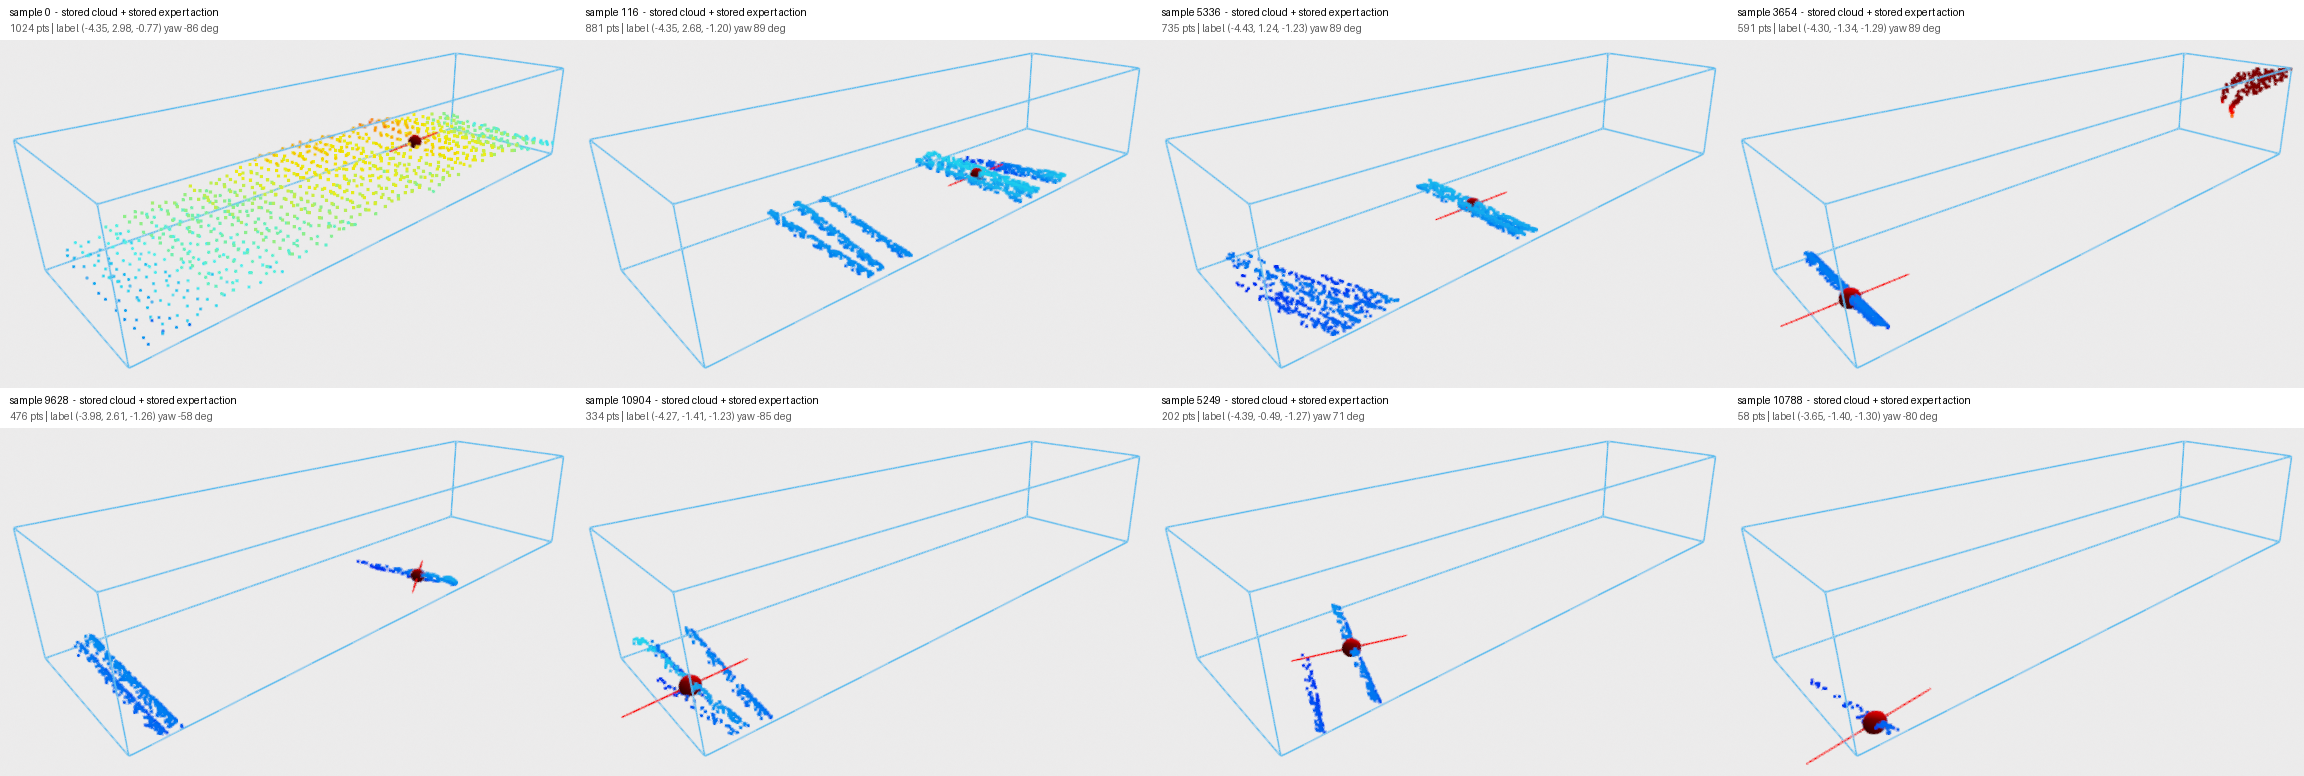
\includegraphics[width=\linewidth]{figures/dataset_samples_aug1v2.png}
\caption{Stored training tuples from a tight-crop dataset after dig
relabeling to $d = 0.25$~m: observed cloud, expert grasp center (sphere), and
commanded yaw (line). The samples span the episode from full pile to
near-empty rack. Most relabeled grasp heights lie in the narrow band at the
bottom of the action box, the flattening that Equation~\eqref{eq:dig}
imposes on the regression $z$ target.}
\label{fig:bc_dataset_samples}
\end{figure}

\subsection{Shape augmentations}

Because early datasets were collected over flat piles, the trainer supports a
family of label-consistent shape augmentations applied per batch in encoded
action space (decode with Equation~\eqref{eq:arctanh_dec}, transform in
meters, re-encode with Equation~\eqref{eq:arctanh_enc}): a vertical shift of
cloud and label by a common $\Delta z \sim \mathcal{U}(0, z_{\max})$ to teach
$z$-equivariance for piles taller than the training distribution, and a mound
warp that reshapes the cloud into a profile peaked at the label position to
teach peak-targeting. With the profiled-pile collection these are no longer
the primary source of shape diversity but remain available. All
augmentations leave zero-padded slots untouched.

\section{The Scoring Policy}
\label{sec:bc_scoring}

\subsection{Motivation: mode averaging under a regression loss}
\label{sec:bc_mode_avg}

The minimizer of the mean-squared error in Equation~\eqref{eq:mse} is the
conditional mean of the label given the observation,
\begin{equation}
  \pi^*(P) = \mathbb{E}\left[ a \mid P \right].
\end{equation}
When the expert's behavior is unimodal this is the right answer. On a pile
with two near-equal mounds it is not: the expert grasps one mound or the
other depending on millimeter-scale height differences, so conditioned on the
observable cloud the label distribution is bimodal, and its mean lies in the
empty gap between the mounds. The policy then commands a grasp over air.

This failure was measured directly. On procedurally generated near-tie
two-mound scenes, the privileged expert and the geometric heuristic (both of
which select a candidate by argmax) aim into the gap in $0\%$ of scenes,
while the regression policy aims into the gap in $33.9\%$ of scenes (and in
$21\%$ of those the commanded grasp closes on nothing); an RL-fine-tuned
regression policy reached $48.5\%$. On the real crane the failure is
absorbing: a grasp over a gap disturbs nothing, so the next observation is
identical and the deterministic policy re-issues the same target, which was
observed for five consecutive cycles in a field trial
(Section~\ref{sec:bc_trials}). In simulation the same
failure costs about three extra cycles per pile, because failed grasps still
nudge logs and eventually let the policy escape.

The scoring policy removes this failure by construction: instead of
regressing coordinates, it classifies \emph{which observed point} to grasp.
A classification loss cannot be minimized by averaging two modes, and an
argmax over observed points cannot select empty space.

\subsection{Architecture}

The scoring policy reuses the PointNet trunk of
Equation~\eqref{eq:pointnet} with identical layer sizes, with one change: the
per-point features $h_i$, which the regression encoder discards at the
max-pool, are returned alongside the pooled global feature $g$. Encoder
weights therefore remain load-compatible between the two policies, and the
frozen-encoder BC-to-RL recipe carries over unchanged.

A shared per-point head conditions each point on the global context. For
every point $i$ the head consumes the concatenation of its per-point feature,
the global feature (after dropout, $p = 0.2$), and its raw coordinates,
\begin{equation}
  e_i = \mathrm{MLP}_{\mathrm{head}}\!\left( \left[ h_i;\, \mathrm{drop}(g);\, p_i \right] \right)
  \in \mathbb{R}^{64},
\end{equation}
with $\mathrm{MLP}_{\mathrm{head}}: 515 \to 128 \to 64$ (ELU activations),
and three linear output heads read off
\begin{equation}
  s_i = w_s^\top e_i \in \mathbb{R}, \qquad
  \delta_i = w_\delta^\top e_i \in \mathbb{R}, \qquad
  q_i = W_q\, e_i \in \mathbb{R}^2,
\end{equation}
a grasp-quality logit $s_i$, a vertical residual $\delta_i$ from the point to
the commanded grasp center, and a per-point yaw $q_i = (q_i^c, q_i^s)$ in the
doubled-angle encoding of Equation~\eqref{eq:yaw_enc}. Padded slots receive
$s_i = -\infty$ so they can never win the argmax. The horizontal coordinates
$x$ and $y$ are not predicted: they are read off the selected point. Depth is predicted
only as a residual from the selected surface point, not as an absolute
coordinate.

\subsection{Label construction and training objective}
\label{sec:bc_scoring_loss}

The scoring policy trains on the same datasets as the regression policy; no
recollection is needed. Stored regression labels are decoded back to metric
targets $(t, \psi)$ with Equations~\eqref{eq:arctanh_dec} and
\eqref{eq:yaw_enc}, and the classification target becomes the observed
(non-padded) point nearest the expert grasp in the horizontal plane:
\begin{equation}
  i^* = \operatorname*{arg\,min}_{i}\; d^{\mathrm{xy}}_i, \qquad
  d^{\mathrm{xy}}_i = \left\lVert p_{i,xy} - t_{xy} \right\rVert_2 .
\end{equation}
Because FPS-sampled neighbors of $i^*$ are often near-identical grasp
candidates, the hard label is smoothed over a horizontal radius
$\rho = 0.12$~m: the target distribution $y$ is uniform over
$\{ i : d^{\mathrm{xy}}_i \le \rho \} \cup \{ i^* \}$ and zero elsewhere. The radius is
smaller than any physical gap between mounds, so smoothing shares probability
among interchangeable neighbors without ever bridging the gap whose avoidance
motivates the classification loss in the first place.

The loss combines cross-entropy on the scores with regression terms evaluated
\emph{only at the labeled point}:
\begin{align}
  \mathcal{L}_{\mathrm{cls}} &= - \sum_{i=1}^{N} y_i \,
      \log \operatorname{softmax}(s)_i, \\
  \mathcal{L}_{\delta} &= \left( \delta_{i^*} - \left( t_z - p_{i^*, z} \right) \right)^2, \qquad
  \mathcal{L}_{\mathrm{yaw}} = \left\lVert q_{i^*} -
      \left( \cos 2\psi,\, \sin 2\psi \right) \right\rVert_2^2, \\
  \mathcal{L}_{\mathrm{score}} &= \mathcal{L}_{\mathrm{cls}}
      + \lambda_\delta \, \mathcal{L}_{\delta}
      + \lambda_{\mathrm{yaw}} \, \mathcal{L}_{\mathrm{yaw}},
  \qquad \lambda_\delta = 1.0, \quad \lambda_{\mathrm{yaw}} = 0.5 .
  \label{eq:scoring_loss}
\end{align}
No per-point annotation is required. The dataset holds one expert grasp per
cloud, the same $(P_k, t_k, \psi_k)$ tuples the regression policy consumes,
and the per-point targets are derived from that grasp at training time.
Three properties follow. First, the scores are not regressed toward
prescribed values: cross-entropy constrains only the softmax-normalized
ranking, so raising the labeled point's score lowers every other point's
normalized probability and the $N - 1$ unlabeled points receive implicit
downward pressure. The head therefore learns a relative log-odds that the
expert would grasp at a point, invariant to a constant offset across the
cloud, which is the quantity the argmax requires. The structure negatives of
Section~\ref{sec:bc_scoring_aug} are the only supervision that lowers
individual scores explicitly. Second, the depth and yaw heads receive
gradient at the labeled point only; their outputs at the remaining points
are unconstrained by Equation~\eqref{eq:scoring_loss} and generalize through
the shared per-point head, which is what makes them usable at whichever
point wins the argmax. Third, the horizontal coordinates are not predicted,
so they require no supervision.

Optimization mirrors the regression policy: AdamW with learning rate
$10^{-4}$ and weight decay $10^{-4}$, batch size 64, an 85\,/\,15 split, a
reduce-on-plateau schedule, per-epoch ZED noise, and best-validation
checkpointing. Alongside the validation loss, training reports the median
horizontal error of the decoded grasp and the fraction of validation scenes
within $0.30$~m of the expert target.

The digging-depth convention of Equation~\eqref{eq:dig} is applied to the
metric label $t_z$ before computing the residual target
$t_z - p_{i^*, z}$. It therefore shifts only the depth head; the
classification target, which point to grasp, is untouched, so the
label-clamping problem of Section~\ref{sec:bc_dig} cannot collapse the
selection signal.

The residual target is close to constant over much of the dataset, which
follows from its construction. Where the clamp in Equation~\eqref{eq:dig} is
inactive and the selected point lies on the same local surface as the label,
$t_z - p_{i^*, z} = -d$ exactly. On the margin dataset used for the deployed
checkpoint ($d = 0.25$~m, floor at $-1.20$~m) the labeled point sits a median
of $0.041$~m from the expert target in the horizontal plane, and the residual
targets have mean $-0.125$~m with standard deviation $0.144$~m. The two
regimes behave differently. On the $42\%$ of samples where the clamp is
inactive the residual is grouped near $-d$ (mean $-0.207$~m, standard
deviation $0.112$~m), the remaining spread coming from log curvature and from
the sampled point not coinciding with the surface height at the label. On the
$58\%$ where the label is pinned to the floor the residual becomes
$z_{\mathrm{floor}} - p_{i^*, z}$ and therefore varies directly with the
height of the selected point (mean $-0.062$~m, standard deviation
$0.134$~m), turning positive where that point lies below the floor plane. The
head thus predicts a near-constant bite depth in the free regime and a
floor-referenced correction in the clamped one. In both regimes the commanded
height is anchored to the selected point rather than to the global frame,
which is the property that makes the parameterization insensitive to pile
height.

\subsection{Inference}

At deployment the grasp is decoded from the highest-scoring admissible point
(Algorithm~\ref{alg:scoring_decode}):
\begin{equation}
  \hat{i} = \operatorname*{arg\,max}_{i \,\in\, \mathcal{C}} s_i, \qquad
  \hat{t} = \left( p_{\hat{i},x},\; p_{\hat{i},y},\; p_{\hat{i},z} + \delta_{\hat{i}} \right), \qquad
  \hat{\psi} = \tfrac{1}{2} \operatorname{atan2}\!\left( q_{\hat{i}}^s,\, q_{\hat{i}}^c \right).
\end{equation}
The \emph{candidate mask} defines the admissible set: $\mathcal{C}$ contains
the non-padded points that lie inside the action box
$[b^{\min}, b^{\max}]$. It is always active, in offline evaluation and in
the deployed node alike, where the box is supplied as a runtime parameter and
set to the same training-coordinate action box the policy was trained
against. The mask is required by the widened observation crop: with
$m > 0$ the input cloud deliberately contains points outside the action box
(bed apron, rack posts and rails, pole bases in the margin band). Those
points are observation \emph{context}, and the network is free to use them to
judge the scene, but they are not commandable grasps, so selecting one would
issue an unreachable or unsafe target. Without the mask, an argmax on a real
cloud selected a margin-band point beside tall structure, outside the
reachable volume. Masking is applied to the
score before the argmax, so a masked point can never win regardless of its
score, and the same rule carries over unchanged to reinforcement learning,
where it becomes exact logit masking in the action distribution.

A second, \emph{optional} filter exists but was not used in any result
reported here. The \emph{support gate} further restricts $\mathcal{C}$ to
points whose local horizontal neighborhood is well populated: with
$n_i = \left| \{ j : \lVert p_{j,xy} - p_{i,xy} \rVert < r_s \} \right|$ and
$r_s = 0.5$~m, a point survives only if $n_i \ge \kappa \max_j n_j$. It was
introduced because a raw argmax can in principle be won by a single
noise-displaced point, a failure characterized in simulation on the
tight-crop policy (Section~\ref{sec:bc_noise_sweep}). The margin-trained
policy did not exhibit that failure, so the gate is disabled by default and
was disabled in both hardware trials and in every number quoted in this
chapter; it is retained only as an opt-in safeguard for the tight-crop
checkpoint. Because it is pure geometric post-processing rather than
learning, keeping it off means the results credit the learned
discrimination alone.

\begin{algorithm}[t]
\caption{Scoring-policy inference with admissibility masking}
\label{alg:scoring_decode}
\begin{algorithmic}
\algin{Observation cloud $P$ with padding mask
(Algorithm~\ref{alg:obs_pipeline}); trained scoring network; action box
$[b^{\min}, b^{\max}]$; support-gate flag (disabled by default).}
\algout{Grasp target $\mathbf{g} = (\hat{t}_x, \hat{t}_y, \hat{t}_z, \hat{\psi})$.}

\algstage{1.\;Forward pass}
\State $\{h_i\}, g \gets \mathrm{PointNet}(P)$
\Comment{per-point features and the pooled global feature}
\State $e_i \gets \mathrm{MLP}_{\mathrm{head}}\big([\,h_i;\, g;\, p_i\,]\big)$ for all $i$
\State $s_i \gets w_s^\top e_i$, \quad
       $\delta_i \gets w_\delta^\top e_i$, \quad
       $q_i \gets W_q e_i$

\algstage{2.\;Admissibility mask}
\State $\mathcal{C} \gets \{\, i : p_i \text{ is not padding and } b^{\min} \preceq p_i \preceq b^{\max} \,\}$
\If{support gate enabled}
  \State $n_i \gets \big| \{ j : \lVert p_{j,xy} - p_{i,xy} \rVert < r_s \} \big|$
  \State $\mathcal{C} \gets \{\, i \in \mathcal{C} : n_i \ge \kappa \max_j n_j \,\}$
  \Comment{off in every result reported here}
\EndIf
\State $s_i \gets -\infty$ for all $i \notin \mathcal{C}$
\Comment{applied to the score, so a masked point can never win}

\algstage{3.\;Decode}
\State $\hat{\imath} \gets \operatorname*{arg\,max}_{i} s_i$
\State $(\hat{t}_x, \hat{t}_y) \gets (p_{\hat{\imath},x},\, p_{\hat{\imath},y})$
\Comment{read off the point, not predicted}
\State $\hat{t}_z \gets p_{\hat{\imath},z} + \delta_{\hat{\imath}}$
\Comment{residual from the selected surface point}
\State $\hat{\psi} \gets \tfrac{1}{2}\operatorname{atan2}(q^s_{\hat{\imath}},\, q^c_{\hat{\imath}})$
\State Clamp $\hat{t}_z$ to the bed-floor envelope (Section~\ref{sec:s2r_deploy})
\State \Return $(\hat{t}_x, \hat{t}_y, \hat{t}_z, \hat{\psi})$
\end{algorithmic}
\end{algorithm}

\subsection{Augmentations specific to the scoring parameterization}
\label{sec:bc_scoring_aug}

Two augmentations exploit or extend the classification structure.

\emph{Rigid horizontal shift.} The cloud and the label are translated by a
common offset drawn uniformly from $[-v, v]$ per axis in $x$ and $y$, with
padded slots left at the origin; the deployed checkpoint used
$v_x = 0.15$~m and $v_y = 0.5$~m. Because the classification label is a
point index, the translation maps the label to itself and no relabeling is
needed, so the augmentation supplies additional samples at no supervision
cost. The same augmentation applied to a regression policy changes the
numeric target and requires it to fit its coordinate map over the enlarged
domain (Section~\ref{sec:bc_differences}). Note that both policies are still
deployed against a calibrated crop box; the augmentation widens the range of
scene positions seen in training, it does not remove the need for
calibration. The vertical axis is not
augmented, because the bed floor and gravity are physical rather than
calibration choices.

\emph{Structure negatives.} The collected margin clouds contain full-height
pole columns, whereas the real rack also presents broken poles cut down to
short stubs. A pole-variation augmentation supplies the missing heights from
the columns already in the data, without recollection and without inserting
synthetic geometry. Pole-like columns are detected once per cloud as
clusters of points reaching above the pile ceiling. Each epoch, with
probability $0.7$ a cloud is varied at all; within a varied cloud each column
draws $u \sim \mathcal{U}(0,1)$ and is kept intact for $u < 0.25$, cut to a
stub of height $\mathcal{U}(0.08, 0.6)$~m for $0.25 \le u \le 0.90$, and cut
nearly flush at $0.05$~m for $u > 0.90$. Points above the cut are removed and
the point count is held fixed by zero padding, so the tensor shape is
unchanged. Cross-entropy alone gives a known-structure point no more downward
pressure than any other non-label point, so the pole points that survive the
draw are additionally driven negative with a softplus penalty on their raw
scores:
\begin{equation}
  \mathcal{L}_{\mathrm{neg}} = \frac{1}{|\mathcal{S}|} \sum_{i \in \mathcal{S}}
  \log\!\left( 1 + e^{s_i} \right),
\end{equation}
added to Equation~\eqref{eq:scoring_loss} with weight $w_{\mathrm{neg}}$,
where $\mathcal{S}$ is the set of pole points surviving the draw
(Figure~\ref{fig:bc_stub_aug}). The scoring policy deployed in the hardware
trials of Section~\ref{sec:bc_trials} was trained with this augmentation and
with the explicit negatives.

\begin{figure}[t]
\centering
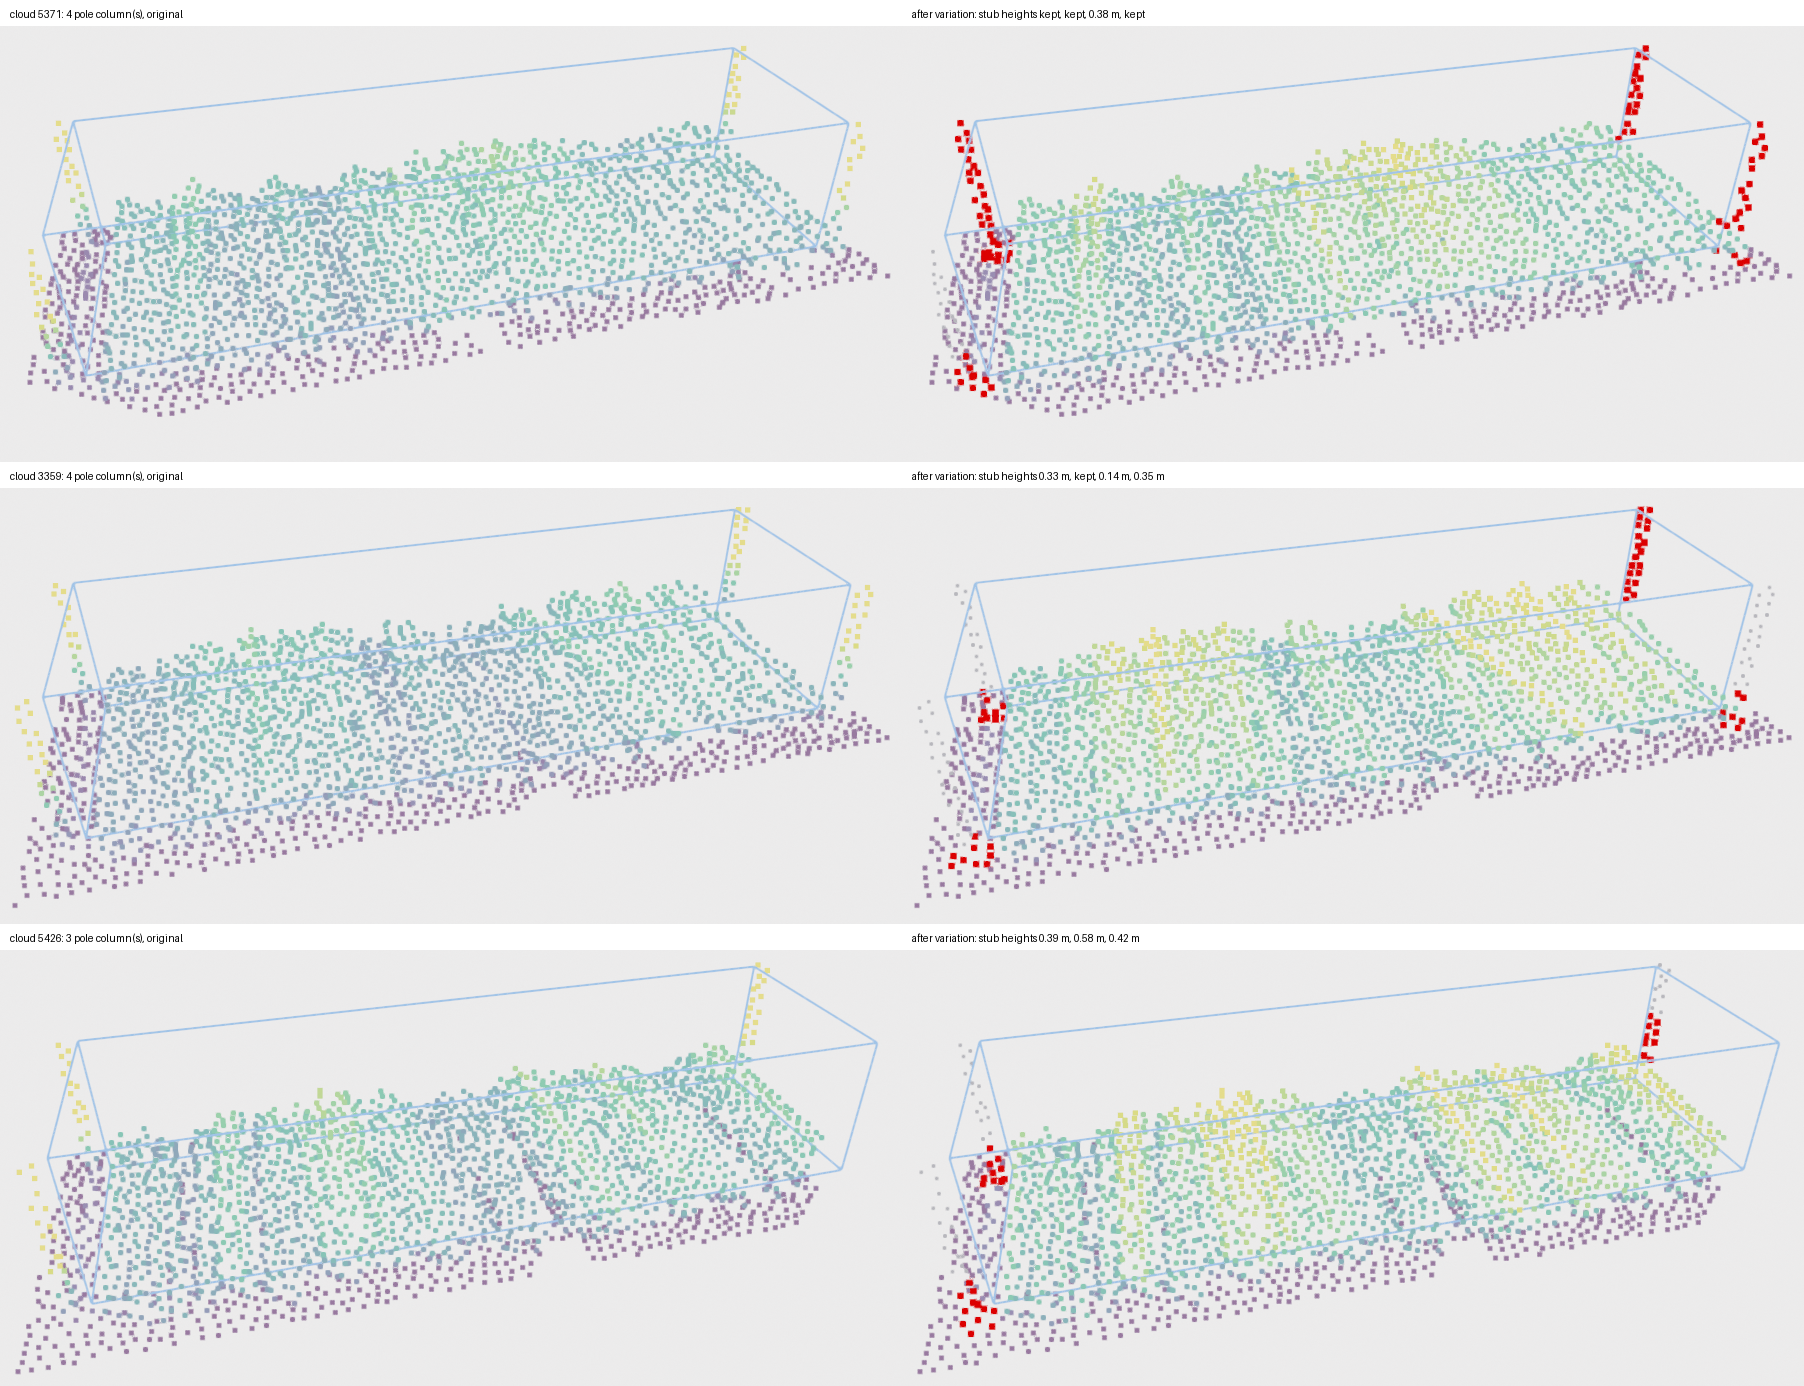
\includegraphics[width=\linewidth]{figures/pole_variation.png}
\caption{Pole-variation augmentation on three margin-dataset clouds (rows).
Left: the collected cloud, with full-height pole columns at the corners of
the crop. Right: one draw of the augmentation, with removed points shown as
grey ghosts at their original positions and the surviving pole points, which
form the negative set $\mathcal{S}$, in red. Realized stub heights are given
per column above each panel; columns drawn as kept retain their full height
and still contribute negatives.}
\label{fig:bc_stub_aug}
\end{figure}

\section{Explicit Differences}
\label{sec:bc_differences}

Table~\ref{tab:bc_differences} summarizes the two policies. Everything
upstream is shared: the same expert, the same datasets, the same cloud
preprocessing, the same noise model, the same PointNet trunk with
load-compatible weights, and the same optimizer settings. The policies differ
in five places, each a consequence of the output parameterization.

\begin{table}[t]
\centering
\caption{Regression versus scoring BC policies. Shared components: expert
demonstrations, datasets, cloud preprocessing, ZED noise augmentation,
PointNet trunk (per-point MLP $3 \to 64 \to 128 \to 256$, max-pool, projection
to $256$), AdamW ($10^{-4}$, weight decay $10^{-4}$), batch size 64,
85\,/\,15 split, plateau schedule, best-validation checkpointing.}
\label{tab:bc_differences}
\begin{tabular}{p{0.24\linewidth} p{0.34\linewidth} p{0.34\linewidth}}
\hline
 & \textbf{Regression} & \textbf{Scoring} \\
\hline
Output & One global 5D vector: box-normalized $\operatorname{artanh}$ $(x,y,z)$, $(\cos 2\psi, \sin 2\psi)$ & Per-point logit $s_i$, depth residual $\delta_i$, yaw $q_i$; grasp read off the argmax point \\
Features used & Global max-pooled feature only & Per-point features and global feature \\
Loss & MSE on the 5D vector, Eq.~\eqref{eq:mse} & Cross-entropy over points + MSE at the labeled point, Eq.~\eqref{eq:scoring_loss} \\
Optimal predictor & Conditional mean of the expert action & Conditional mode over observed points \\
Multimodal scenes & Averages modes; can aim into the gap between mounds & Commits to one mound; target always on observed material \\
Depth & Absolute $z$ in the action box & Residual from the selected surface point \\
Dig relabeling & Floor clamp flattens $z$ labels; couples into the joint loss & Affects the residual head only; selection signal untouched \\
Translation & Coordinates are learned; an uncorrected frame shift displaces the command & Label is an index; rigid-shift augmentation needs no relabeling, and $x, y$ are read off a point rather than extrapolated \\
Inference & Decode, Eq.~\eqref{eq:arctanh_dec}; no masking needed & Candidate mask to the action box (always on); support gate available but unused \\
\hline
\end{tabular}
\end{table}

\subsection{Estimator: mean versus mode}

This is the root difference; the rest follow from it. The regression loss is
minimized by the conditional mean of the expert action, the scoring loss by
the conditional mode over observed points
(Section~\ref{sec:bc_mode_avg}). On unimodal scenes the two agree, and the
policies behave near-identically. On multimodal scenes the mean falls between
modes while the mode commits to one. Replayed on the 26 clouds from the field
trial in which the regression policy locked onto the gap between two mounds,
the scoring policy committed to a mound on 26 of 26 clouds with zero
zero-support targets, against a $27\%$ zero-support rate for the regression
policy on the same clouds. The prediction also held on hardware: on the
double-mound shape where the deployed regression policy executed 15 gap
shots in 26 cycles, the deployed scoring policy produced zero gap-targeting
cycles in 30 (Section~\ref{sec:bc_scoring_trials}).

\subsection{Output space: coordinates versus observed points}

The regression policy can output any point in the action box, including empty
space; the scoring policy can only output observed material (plus a small
learned depth residual). This makes the gap-targeting failure impossible
rather than merely unlikely, but introduces an admissibility concern the
regression policy never has: since any observed point could in principle win,
padded and out-of-box points must be excluded explicitly, which is the
candidate mask. The regression policy needs no equivalent because its
$\tanh$ decode confines its output to the action box by construction. In
effect the regression policy's failure mode is averaging, and the scoring
policy's residual failure mode is trusting a single bad candidate; the
candidate mask closes the reachability half of that, and the optional support
gate exists for the noise half, though the deployed policy did not need it.

\subsection{Depth: absolute versus residual}

Regressing absolute $z$ ties the depth prediction to the global frame and to
the label distribution, which the dig-relabeling clamp then flattens
(Section~\ref{sec:bc_dig}). Predicting a residual from the selected surface
point makes depth local: the network learns "how far below this surface to
bite," which transfers across pile heights and is unaffected by where the
labels sit relative to the floor. The residual parameterization also
sidesteps the $z$-saturation seen when real piles were taller than any sim
training pile, a failure that previously required a dedicated
$z$-shift augmentation for the regression policy.

\subsection{Frame sensitivity}

Neither network is translation invariant: both consume raw coordinates, and
the scoring head concatenates $p_i$ to its per-point input. The difference
lies in what a rigid horizontal shift does to the label and to the output.

For the regression policy the shift changes the label, since the target is a
metric coordinate. The practical consequence appeared when the rack was found
to sit about $0.45$~m in $y$ from the position at which the crop box had been
calibrated. Correcting this is ordinary recalibration, not a policy
mechanism: the offset is measured once and applied as a parameter that
translates the crop box onto the rack, returns the cropped cloud to the
coordinates the network was trained in, and adds the offset back to the
decoded command. What the episode measured is the sensitivity itself. Moving
the crop box by the rack offset without returning the cloud to training
coordinates displaced the regression policy's commanded target by $1.2$ to
$1.6$~m, several times the physical displacement, which shows how tightly a
regressed coordinate is bound to the frame it was trained in.

For the scoring policy the shift leaves the label unchanged, because the
label is a point index rather than a coordinate: translating cloud and label
together maps $i^*$ to itself. The augmentation is therefore label preserving
and generated at no cost, and the deployed checkpoint was trained with
offsets drawn uniformly from $\pm 0.15$~m in $x$ and $\pm 0.5$~m in $y$. The
second effect is on the output path. The horizontal command is read from the
selected point instead of extrapolated from a learned coordinate map, so a
shift can only act through the ranking, and a ranking error that moves the
argmax to a neighboring point on the same material still yields a target on
material. This bounds the failure rather than removing it. The score function
remains shift sensitive through $p_i$, the depth residual and yaw are not
protected by the index argument, and the hardware trials of
Section~\ref{sec:bc_scoring_trials} still ran with the measured rack offset
applied, so
this is a property of the parameterization and not a measured deployment
result.

\subsection{Architecture and BC-to-RL compatibility}

The trunks are identical up to the max-pool, and layer names are
load-compatible; the scoring policy simply keeps the per-point features that
the regression encoder discards. Head capacity differs modestly: the
regression head is an MLP on the global feature, while the scoring head is a
shared per-point MLP on a $515$-dimensional input (per-point feature, global
feature, raw coordinates) with three linear outputs. Because the encoder is
shared and unchanged, the frozen-encoder BC-to-RL fine-tuning recipe
developed for the regression policy applies to the scoring policy without
modification.

\section{Field Trials and Analysis}
\label{sec:bc_trials}

This section reports the hardware evidence: a baseline campaign with the
deployed geometric heuristic whose failure analysis fixed the priorities for
the scoring design, offline replays of both learned policies on the recorded
clouds from those trials, a simulated observation-degradation sweep, and two
hardware trials of the scoring policy. Throughout, a \emph{cycle} is one
grasp-transport-deposit sequence, \emph{success rate} is the fraction of
cycles that deposit at least one log, and \emph{alignment} is an
operator-assigned score from 1 to 5 for how well the grapple met the logs.
Deposition in every trial follows the bin-fill procedure of
Section~\ref{sec:s2r_deposit}.

\subsection{Baseline campaign and failure taxonomy}
\label{sec:bc_baseline_trials}

Three trials of the deployed perception heuristic were run on approximately
200-log piles arranged in three shapes: a double mound, a jagged multi-peak
profile, and a single mound (Table~\ref{tab:bc_baseline_trials}). Pooled, the
baseline grasped at least one log on 67\% of 73 cycles. The jagged profile is
the hard geometry, needing roughly twice the cycles of the mound shapes for
the same inventory.

\begin{table}[t]
\centering
\caption{Baseline (geometric heuristic) field trials. Success is the
fraction of cycles depositing at least one log; $c_{95}$ is the cycle at
which 95\% of the eventually-moved logs had been moved; alignment is the
operator score (1--5).}
\label{tab:bc_baseline_trials}
\begin{tabular}{lcccccc}
\hline
\textbf{Trial} & \textbf{Cycles} & \textbf{Logs} & \textbf{Success \%} &
\textbf{Logs/success} & $c_{95}$ & \textbf{Align.} \\
\hline
Double mound & 18 & 196 & 83.3 & 13.1 & 16 & 4.53 \\
Jagged       & 36 & 193 & 55.6 &  9.7 & 32 & 4.65 \\
Single mound & 19 & 175 & 73.7 & 12.5 & 14 & 4.07 \\
\hline
Pooled       & 73 & 564 & 67.1 & 11.5 & -- & 4.45 \\
\hline
\end{tabular}
\end{table}

Of the 24 empty cycles, 16
(67\% of failures, 22\% of \emph{all} cycles) were caused by the heuristic
targeting rack rails, pole columns, or noise points in the air; 4 were chokes
(grasping too deep for the grapple to close); and 4 were yaw or control
faults. Structure and noise targeting is thus the dominant real-world failure
mode, and it concentrates in the endgame: these failures occurred on average
76\% of the way through a trial (median 82\%), with 11 of 16 in the final
30\% of cycles. The mechanism is geometric. Once the pile drops below the
rack rail height, the rails and poles become the highest points in the crop,
and a highest-point heuristic locks onto them. The failure is absorbing:
grasping a rail changes nothing, so the next cloud is identical and the same
target is reissued. The single-mound trial ended in four consecutive rack
grabs and required manual completion; the jagged trial ended in three.

\begin{figure}[t]
\centering
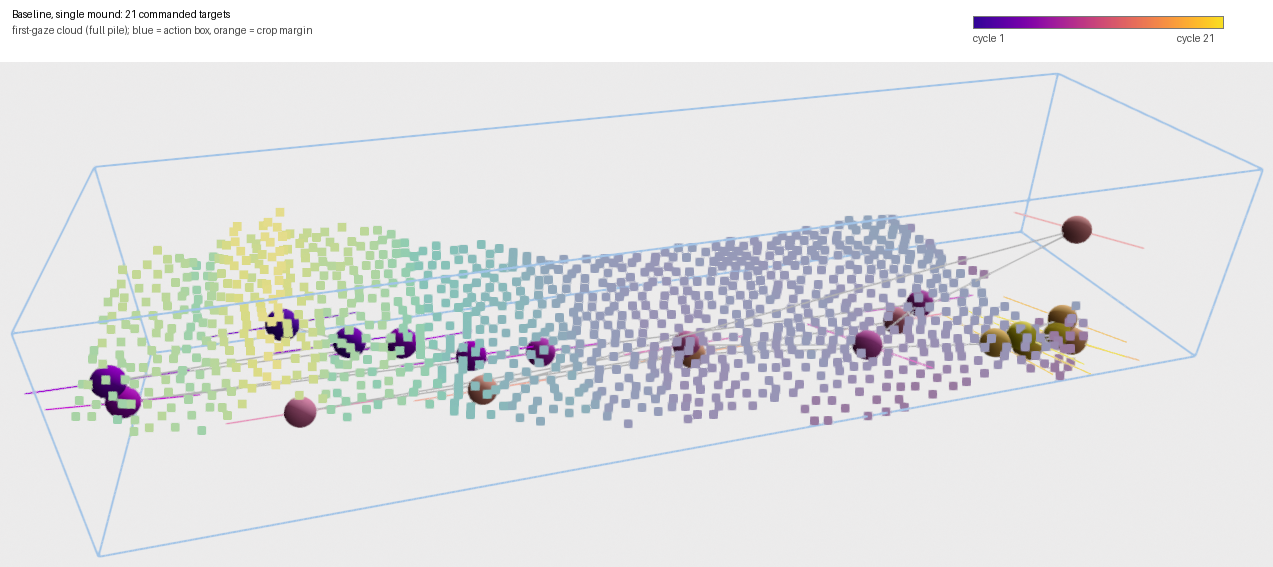
\includegraphics[width=\linewidth]{figures/real_trials/targets_3d_baseline_single.png}
\caption{Every target commanded by the baseline in the single-mound trial,
drawn over the cloud observed at the first cycle. Sphere colour encodes cycle
order, the short line through each sphere is the commanded grapple yaw, and
the blue box is the action volume. Early targets sit on the mound; the final
cycles collapse into a cluster at the far end of the rack, where the end
board and corner poles stand, which is the absorbing lock-in that ended the
trial.}
\label{fig:bc_targets_baseline}
\end{figure}

This taxonomy set the priorities for the scoring policy line: the dominant
failure is a \emph{perception discrimination} failure (log material versus
structure and noise), which is exactly what a learned per-point score can
address, and which motivated the margin crop
(Figure~\ref{fig:bc_sim_vs_real_crop}), the structure negatives
(Section~\ref{sec:bc_scoring_aug}), and the candidate mask.

\subsection{Offline replay on recorded trial clouds}
\label{sec:bc_replay}

Before new hardware time was spent, both policies were replayed offline on
two sets of real clouds: the 26 recorded clouds from the field run in which
the deployed regression policy locked onto the gap between two mounds
(Section~\ref{sec:bc_mode_avg}), and clouds extracted from the baseline
trials' recorded bags, each processed by the pipeline matching the policy
(tight crop at 1024 points, or margin crop at 2048).

On the 26 gap-failure clouds the scoring policy committed to one of the two
mounds on 26 of 26 clouds with zero unsupported targets, against a 27\%
zero-support rate for the regression policy on the same clouds. On the
baseline-trial clouds the qualitative difference is the one predicted by the
estimator argument (Figure~\ref{fig:bc_target_comparison}): the regression
policy places targets at intermediate coordinates between mounds, while the
margin-trained scoring policy selects a point on one mound. The replay also
exposed a genuine weakness of the \emph{tight-crop} scoring variant: on real
clouds it repeatedly selected points on the end board that closes the rack
and on the corner pole columns,
structure it had never observed during training, which is the sim-to-real
asymmetry of Figure~\ref{fig:bc_sim_vs_real_crop} and the reason the
margin-trained variant became the deployment candidate.

\begin{figure}[t]
\centering
\begin{minipage}{0.49\linewidth}
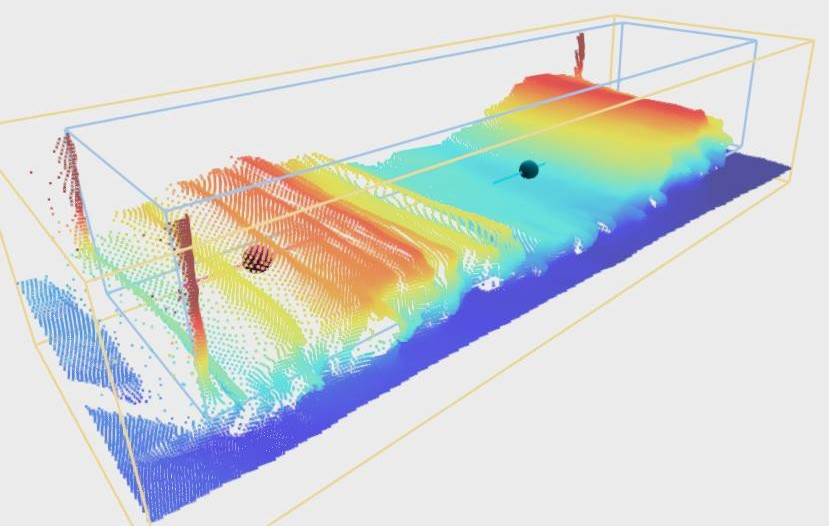
\includegraphics[width=\linewidth]{figures/targets_double_c01.jpg}
\end{minipage}\hfill
\begin{minipage}{0.49\linewidth}
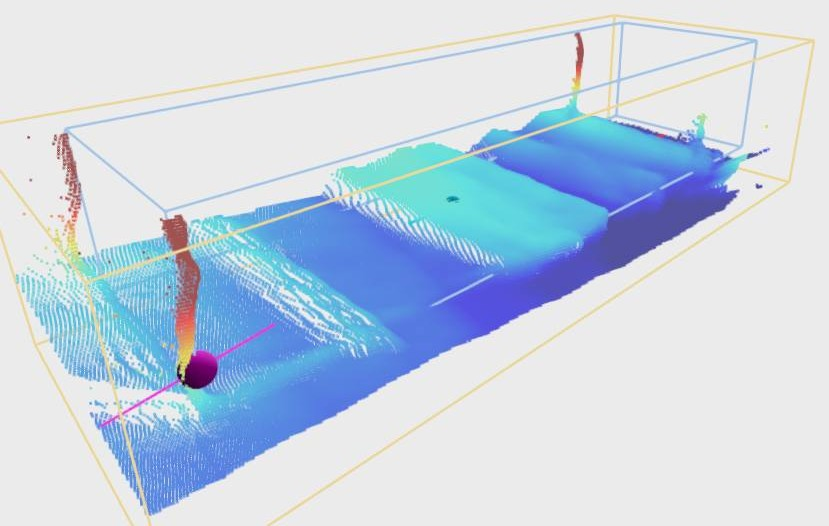
\includegraphics[width=\linewidth]{figures/targets_double_c11.jpg}
\end{minipage}
\caption{Offline policy targets on two recorded double-mound trial clouds
(blue box: action volume; orange box: margin crop; sphere: commanded grasp;
line: commanded yaw). Left: the regression policy (cyan, $y = 2.25$~m) places
its target in the saddle between the two mounds, the conditional-mean
behavior of Section~\ref{sec:bc_mode_avg}, while the margin-trained scoring
policy (red, $y = 3.81$~m) commits to a mound. Right: the tight-crop scoring
variant (magenta) selects a point on a pole column it never saw during
training, while the margin-trained variant, which trains with such structure
in view, targets pile material.}
\label{fig:bc_target_comparison}
\end{figure}

\subsection{Robustness to observation degradation}
\label{sec:bc_noise_sweep}

A simulated sweep scales the axial noise model of
Section~\ref{sec:bc_noise} from clean to $8\times$ the characterized ZED
coefficient (Table~\ref{tab:bc_noise_sweep}). Two results are relevant here.
First, on clean observations the tight-crop scoring policy is the strongest
policy in the comparison (93\% grasp success versus 81\% for the regression
policy). Second, its \emph{ungated} argmax collapses already at the
characterized noise level ($1\times$): a single noise-displaced point can win
the argmax, and the empty cycles' issued targets had a median local support
of 3 points versus 56 for successful ones. This is the collapse that
motivated the support gate of Section~\ref{sec:bc_scoring}. On the exact
collapse clouds the gate raises the empty-cycle target support from 3 to 40
while leaving successful targets unmoved (median displacement 0.00~m). The
margin-trained scoring policy, whose training distribution includes the
structure and clutter that make isolated points plausible, issued zero
unsupported picks in 208 in-distribution noise draws with the gate off; the
gate is therefore kept as opt-in processing rather than a default, and all
hardware trials below ran without it.

\begin{table}[t]
\centering
\caption{Grasp success (\%) under scaled sensor noise in simulation, 10
episodes per cell (sampling spread roughly $\pm 8$--$10$ points per cell).
The scoring row is the tight-crop variant with the support gate off; its
collapse at $1\times$ is the isolated-point argmax failure discussed in the
text, not a discrimination failure.}
\label{tab:bc_noise_sweep}
\begin{tabular}{lcccc}
\hline
\textbf{Policy} & \textbf{Clean} & $1\times$ & $3\times$ & $8\times$ \\
\hline
Geometric heuristic       & 83.5 & 87.4 & 82.9 & 34.0 \\
Regression BC             & 81.1 & 69.4 & 53.7 & 57.0 \\
Scoring BC (tight, ungated) & 93.1 & 49.7 & 20.0 & 35.3 \\
\hline
\end{tabular}
\end{table}

\subsection{Hardware trials of the scoring policy}
\label{sec:bc_scoring_trials}

The margin-trained scoring policy with structure negatives was deployed on
the crane for two trials under the baseline protocol (identical cloud
processing, support gate off). The first trial repeated the single-mound
shape as a paired comparison; the second used the double-mound shape on
which the deployed regression policy had produced the gap-targeting failure
run. Table~\ref{tab:bc_scoring_trials} summarizes both against the matching
baseline trials.

\begin{table}[t]
\centering
\caption{Scoring-policy hardware trials versus the matching baseline trials.
Outcome notes how the trial ended.}
\label{tab:bc_scoring_trials}
\small
\setlength{\tabcolsep}{4pt}
\begin{tabular}{llccccl}
\hline
\textbf{Shape} & \textbf{Policy} & \textbf{Cycles} & \textbf{Logs} &
\textbf{Success \%} & \textbf{Align.} & \textbf{Outcome} \\
\hline
Single mound & Heuristic & 19 & 175 & 73.7 & 4.07 & abandoned in 4 rack grabs \\
Single mound & Scoring   & 23 & 174 & 69.6 & 4.25 & cleared, no assist \\
\hline
Double mound & Heuristic & 18 & 196 & 83.3 & 4.53 & cleared \\
Double mound & Scoring   & 30 & 215/216 & 56.7 & 4.00 & cleared to 1 log \\
\hline
\end{tabular}
\end{table}

On the single mound the per-cycle numbers are comparable (69.6\% versus
73.7\% success), but the trial-level outcomes differ where the baseline
analysis said they would. Both policies hit roughly four structure-noise
cycles; the difference is absorption. The baseline entered its rack-grab
loop and never left, ending the trial with a manual finish. The scoring
policy interleaved real grasps between its structure cycles, escaped each
loop, and cleared the pile completely with no human assistance, where the
paired baseline trial on the same shape had to be abandoned.

The double-mound trial confirms the mode-seeking fix on hardware. On the
shape where the deployed regression policy had executed 15 gap shots in 26
cycles, the scoring policy produced \emph{zero} gap-targeting cycles in 30,
and every executed target sat on well-populated material (local support 40
to 93 points, median 69, with the gate off). Its lower success rate on this
shape has a known decomposition: four to five chokes on the steep right
mound (a deep-dig hardware failure mode that the simulator does not
reproduce, suggesting the fixed $d = 0.25$~m digging depth is too deep for
steep mounds), one yaw fault, and eight endgame structure-noise cycles in
the same end-of-rack region, the residual class that the pending real-data
fine-tuning targets. A replay of both trials with the deployment corner filters disabled
changed 6 of 54 targets (11\%), mostly benign mound-to-mound flips,
indicating the learned discrimination rather than the filters carries most
of the structure avoidance, though the filters still carve away part of the
end-of-rack region.

Figure~\ref{fig:bc_clearing_grid} shows the double-mound trial cycle by
cycle, pairing what the machine did with what the policy saw. Read in
sequence it makes the endgame failure class concrete: while the pile stands
above the rack rails the scored maximum sits on the mound and the commanded
target follows the material down, but from cycle~20, once the remaining logs
drop below the rails, the highest-scoring region migrates onto the rack
structure at the far end of the bunk and stays there, producing the run of
empty cycles that closes the trial. The successful cycles interleaved among
them (22, 24, 27) are what distinguishes this behavior from the baseline's
absorbing loop: the policy leaves the structure, takes real material, and
returns.

\begin{figure}[p]
\centering
\makebox[\linewidth][c]{%
  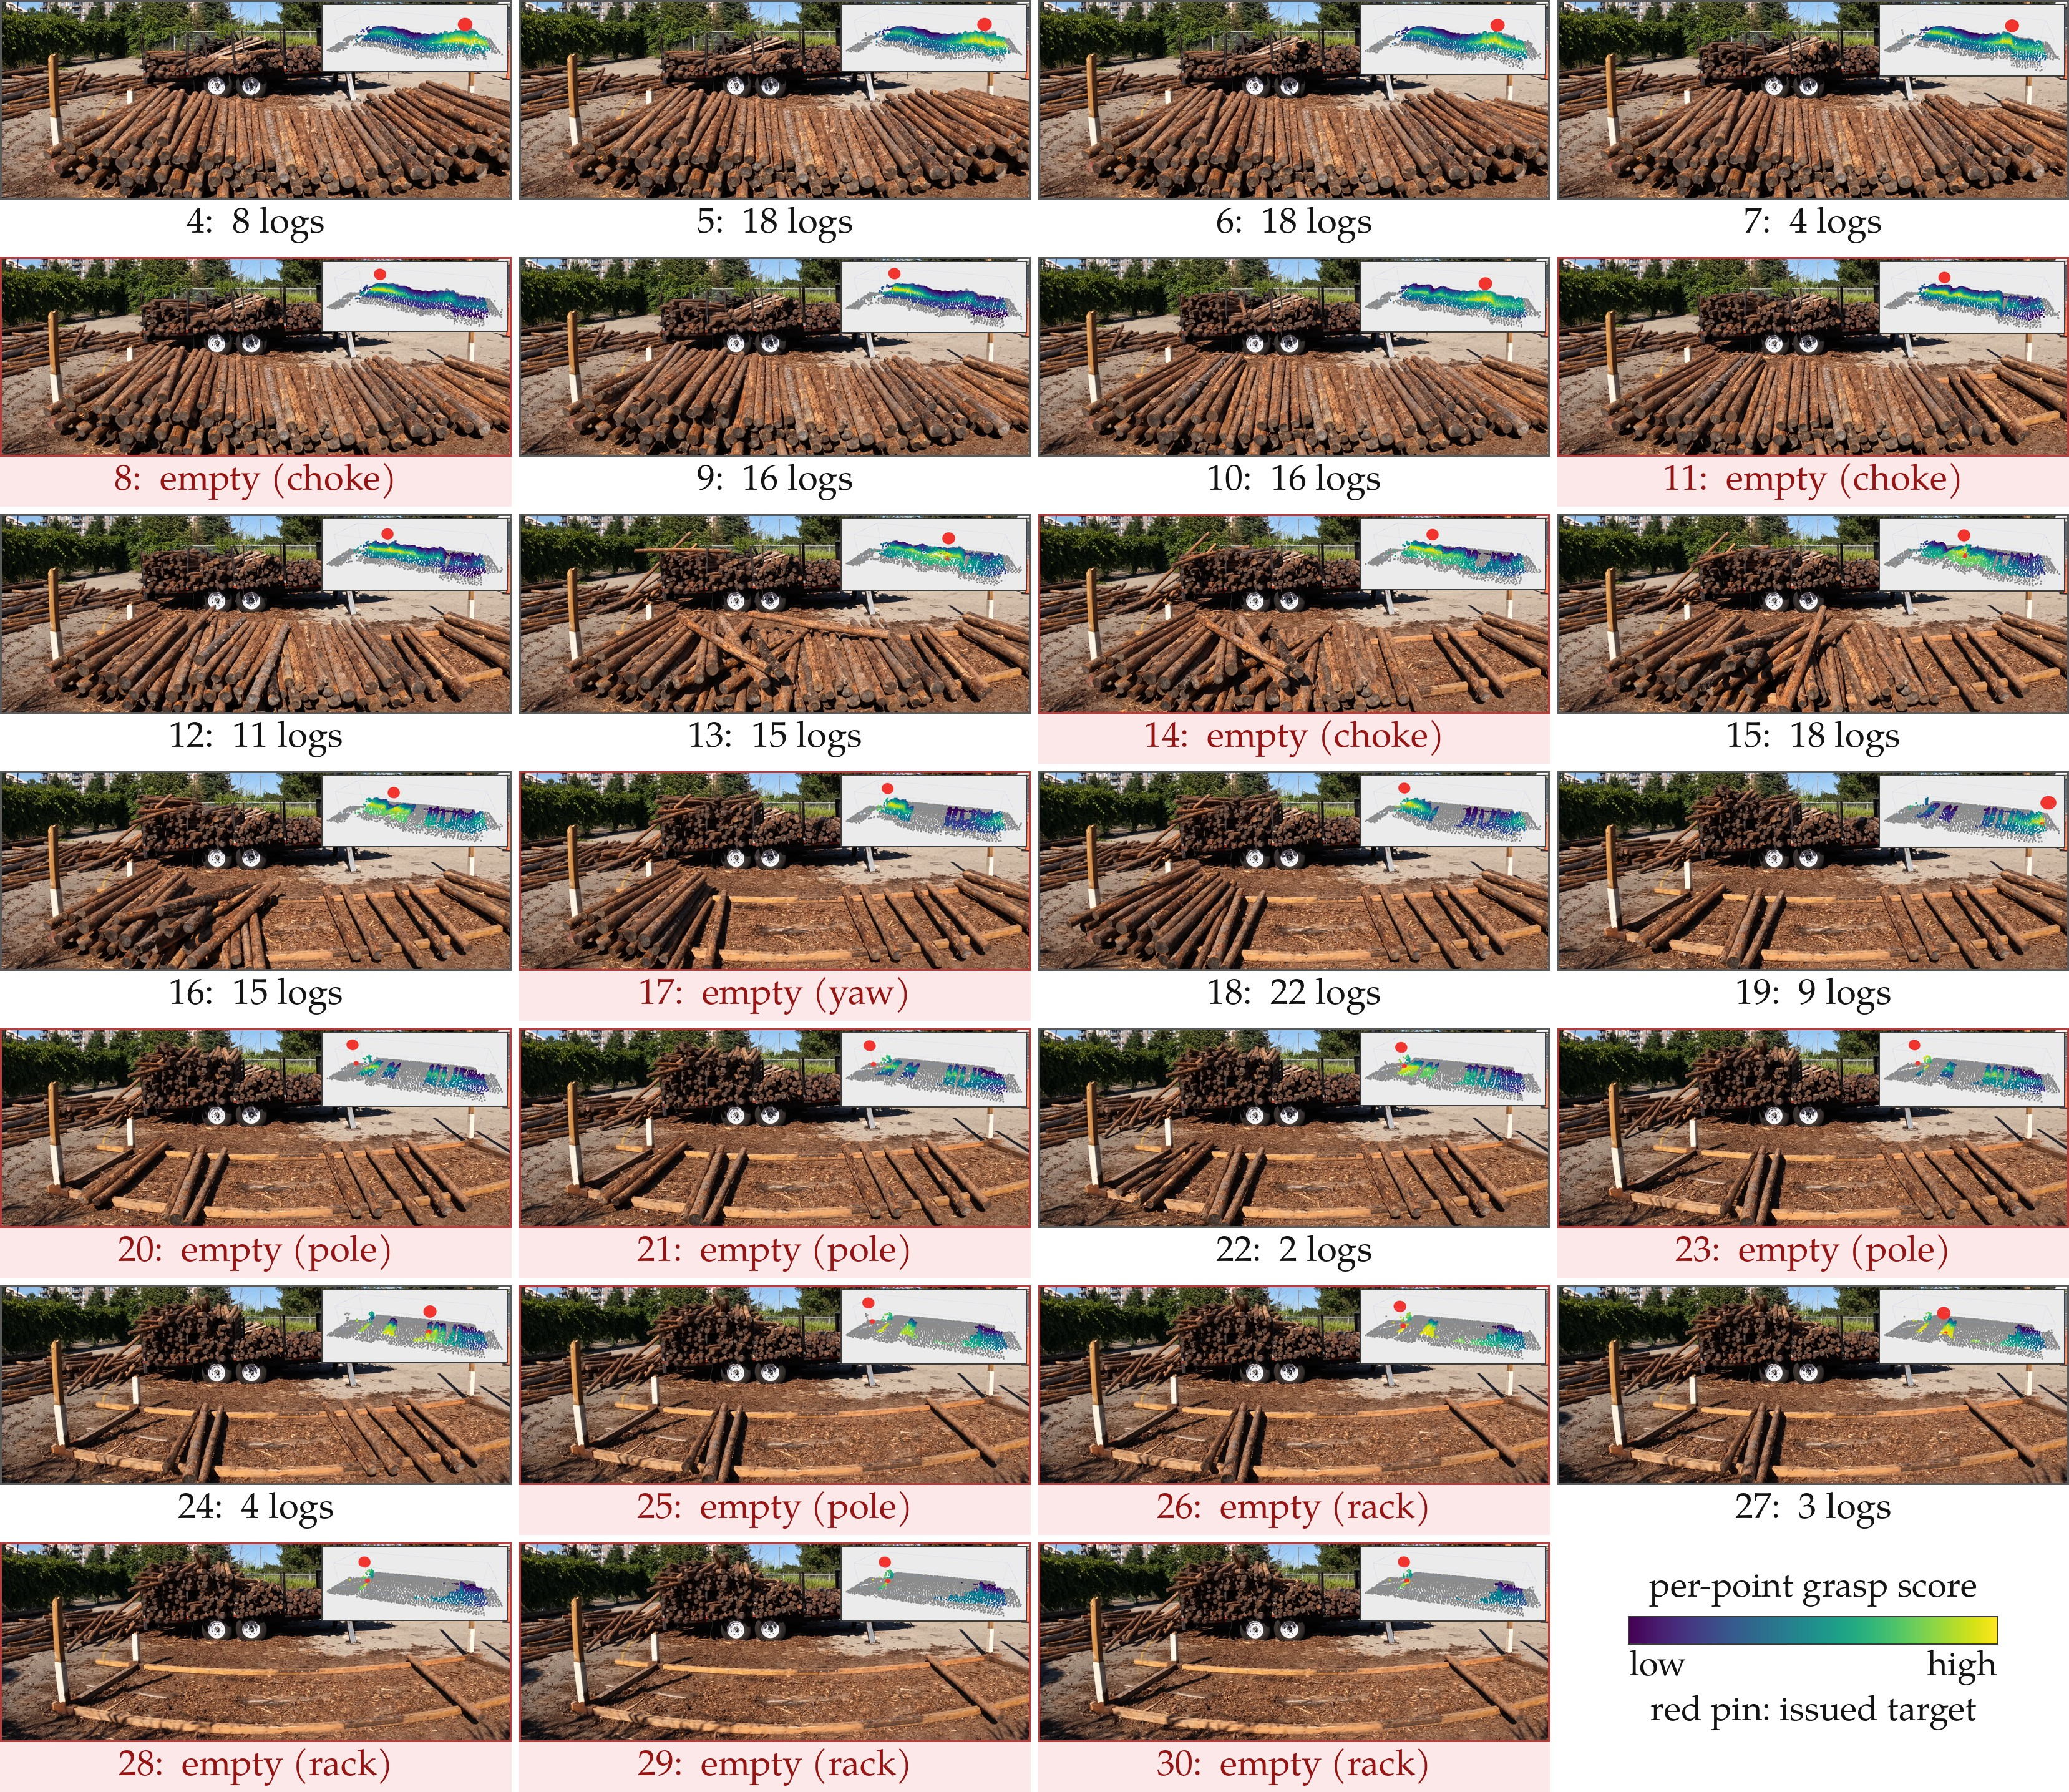
\includegraphics[width=1.12\linewidth]{figures/real_trials/clearing_grid.jpg}}
\caption{The double-mound scoring trial, one panel per grasp cycle. Each
photograph is the frame of a fixed timelapse camera at that cycle's logged
decision time; the inset is the point cloud the policy actually consumed at
that decision, colored by its per-point grasp score, with points outside the
action box (observation context, not commandable) in gray and the issued
target marked by the red pin. The cloud is drawn from the timelapse camera's
side of the rack, so left and right correspond between the photograph and the
inset. Scores are recomputed offline from the
deployed checkpoint and reproduce the logged targets. Panel labels give the
logs moved, scored from the trial record; empty cycles are tinted and
annotated with their cause. Cycles 1 to 3 preceded the start of the
recording. The rack being cleared is the ground-level bunk in the
foreground; the trailer behind it is the deposit target.}
\label{fig:bc_clearing_grid}
\end{figure}

\begin{figure}[t]
\centering
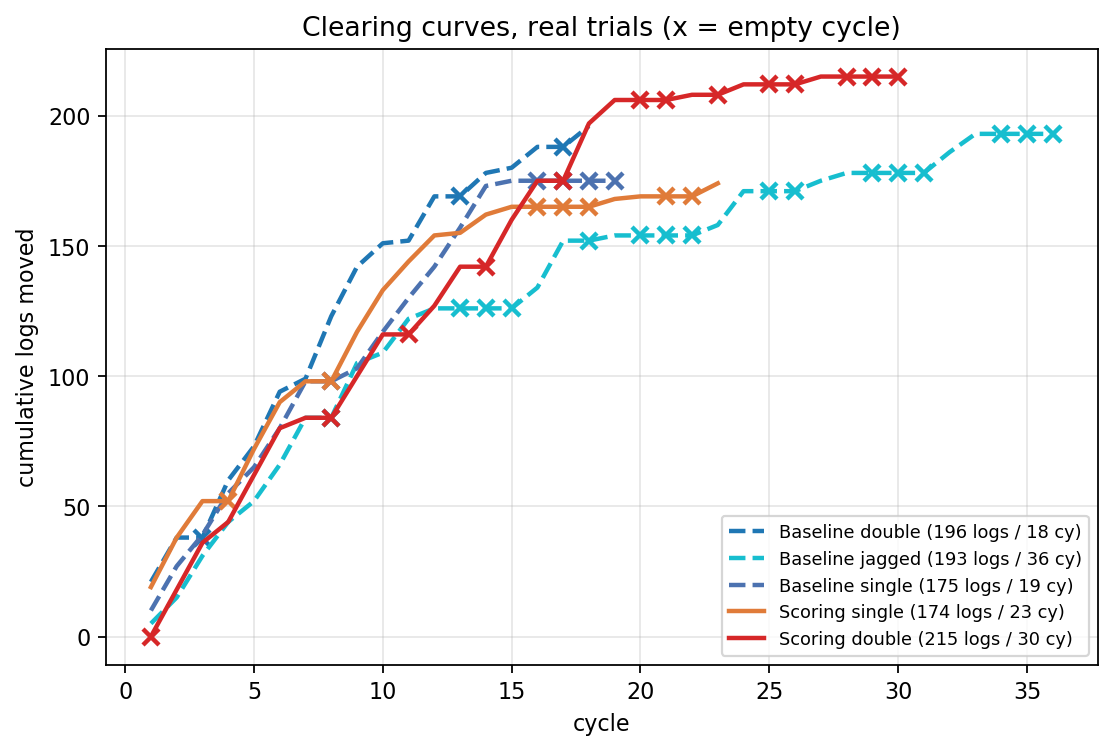
\includegraphics[width=0.92\linewidth]{figures/real_trials/clearing_curves_real.png}
\caption{Cumulative logs moved against cycle for all five trials; crosses
mark empty cycles. The baseline single-mound trial (dashed) flattens into an
unbroken run of empty cycles and was abandoned, while the scoring trials
continue to make progress through their empty cycles and finish their piles.}
\label{fig:bc_clearing_real}
\end{figure}

\begin{figure}[t]
\centering
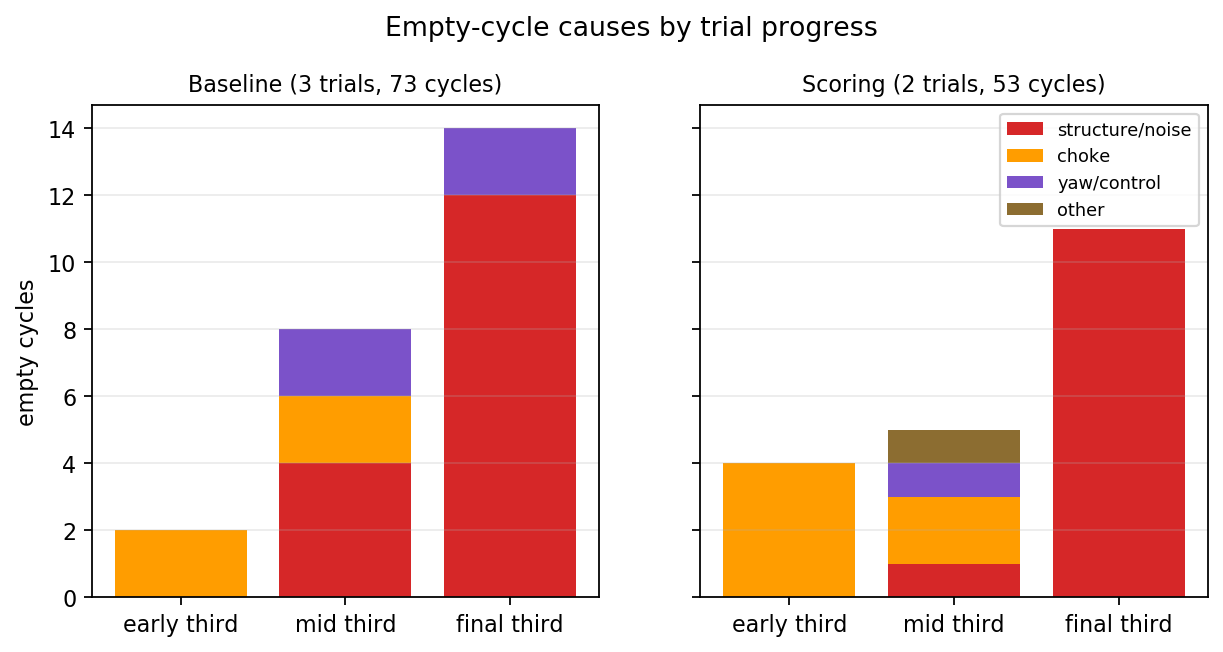
\includegraphics[width=0.92\linewidth]{figures/real_trials/failure_taxonomy_terciles.png}
\caption{Causes of empty cycles by position within the trial, pooled over the
three baseline trials (left) and the two scoring trials (right). Structure
and noise targeting concentrates in the final third for both policies, which
is where the pile falls below the rack rails; chokes are the failure class
the scoring trials added, and are a grapple-closing limit rather than a
perception error.}
\label{fig:bc_taxonomy_real}
\end{figure}

Two conclusions carry forward. The failure class that dominated the baseline
campaign and terminated trials (absorbing structure targeting) is removed or
made escapable by the scoring policy, on hardware, with the gate off, and the
gap-targeting failure of the regression policy did not occur in 30 cycles on
the shape that reliably induced it. The remaining failure classes are a depth
convention (chokes on steep mounds) and endgame structure discrimination in
the end-of-rack region, both addressable in training rather than architecture.

\section{Summary}

Both policies clone the same privileged expert from the same point-cloud
observations with the same trunk and optimizer. The regression policy is the
simpler estimator: one global feature, one 5D vector, one MSE loss. It is
accurate on unimodal scenes but, as the conditional mean, it averages when
the expert's behavior is multimodal, and on the crane that produces an
absorbing grasp-over-the-gap failure. The scoring policy replaces the
coordinate regression with a classification over observed points plus local
depth and yaw regression at the selected point. It is mode-seeking by
construction, keeps its targets on observed material, decouples target
selection from depth conventions, and admits a label-preserving translation
augmentation the regression parameterization cannot exploit, at the cost of
one piece of inference-time admissibility processing the regression policy
does not need: a candidate mask restricting the argmax to the action box.

The field evidence supports the design. The baseline campaign identified
absorbing structure and noise targeting as the dominant real failure mode
(22\% of all cycles, concentrated in the endgame), and the deployed scoring
policy either avoided it or escaped it on hardware: an unassisted full clear
on the shape that had forced the baseline to be abandoned, and zero
gap-targeting cycles on the shape that had reliably induced the regression
policy's mode-averaging failure. What remains is a depth convention (chokes
on steep mounds) and residual endgame discrimination at the end of the rack,
both training-data problems rather than parameterization problems.

% Thesis chapter: reinforcement learning fine-tuning of the behavior-cloned policies.
% Standalone chapter file; \input or \include from the thesis root after the BC chapter
% (cross-references ch:bc_policies and its sections).
% Requires amsmath, amssymb.
% Sources: source/crane_testbed/crane_testbed/agents/scoring_actor_critic.py (P3 actor-critic),
%          scripts/rsl_rl/train.py (fine-tuning entry point, checkpoint load, freezing),
%          scripts/envs/crane_rl_env_gaze.py (_compute_grasp_reward, stability),
%          source/crane_testbed/crane_testbed/tasks.py (task and reward variants),
%          logs/rsl_rl/crane_pointcloud_gaze_scoring_ppo_v0/ (run configuration).

\chapter{Reinforcement Learning Fine-Tuning}
\label{ch:bcrl}

The policies of Chapter~\ref{ch:bc_policies} are trained to imitate a
privileged expert. Imitation has a structural ceiling: the student is graded
on matching the expert's action, not on the outcome of its own, so it
inherits the expert's confidence without the expert's information, and it can
never exceed the strategy it copies. Reinforcement learning removes both
limits by optimizing the task objective directly, under the observations the
policy actually receives. This chapter describes how the behavior-cloned
policies are fine-tuned with on-policy reinforcement learning: the first
generation of fine-tuning on the regression policy, the lessons it produced,
and the current architecture, which fine-tunes the scoring policy with a
categorical action distribution over observed points so that exploration and
credit assignment inherit the properties that motivated the scoring
parameterization in the first place.

\section{Why Fine-Tune, and Why Not RL Alone}
\label{sec:rl_motivation}

Two empirical facts frame the design. First, reinforcement learning from
scratch does not solve this task: across observation types, PPO from random
initialization plateaus around 56\% pile clearing, far below any
behavior-cloned policy. The reward is sparse (one grasp outcome per cycle),
the observation is high-dimensional, and random exploration in grasp space
rarely produces the informative successes that would shape the encoder. A
behavior-cloned initialization supplies what exploration cannot: a policy
that already grasps competently, so that every rollout produces meaningful
outcome signal.

Second, imitation alone optimizes the wrong quantity. The BC loss measures
distance to the expert's command, not grasp outcome. Two consequences follow.
The policy inherits expert behavior that is optimal only under privileged
information (the expert reads ground-truth log poses; the student sees an
occluded, noisy cloud), and it has no mechanism to price its own failure
modes: an empty grasp and a full one are equally acceptable to the imitation
loss as long as the commanded coordinates match the label. Fine-tuning with
task reward lets the policy trade expert fidelity for outcome where its own
observations support the trade, and penalizes exactly the failure modes
(empty cycles, unstable loads, misaligned grasps) that the field trials of
Section~\ref{sec:bc_trials} exposed.

\section{First Generation: Gaussian Fine-Tuning of the Regression Policy}
\label{sec:rl_gen1}

The first fine-tuning recipe wrapped the regression policy of
Section~\ref{sec:bc_regression} in a diagonal Gaussian and ran PPO on the
5D action of Equation~\eqref{eq:arctanh_enc}:
\begin{equation}
  \pi_\theta(a \mid P) = \mathcal{N}\!\left( \mu_\theta(P),\;
  \operatorname{diag}(\sigma^2) \right),
\end{equation}
with $\mu_\theta$ initialized from the BC checkpoint and $\sigma$ initialized
small ($0.05$). Three components of this recipe were validated and carry
forward unchanged in spirit:

\begin{itemize}
\item \emph{Asymmetric critic.} The value function does not read the point
cloud. It is a separate MLP on a privileged state vector (the poses of the
highest logs, Section~\ref{sec:rl_critic}), which learns value quickly and
supplies low-variance advantages from the first iterations of a short
fine-tune, and whose gradients never touch the features the BC actor relies
on.
\item \emph{Frozen encoder.} The PointNet trunk is frozen, including its
batch-normalization statistics; only the actor head moves. Fine-tunes that
unfroze the encoder degraded the policy before reward feedback could
compensate.
\item \emph{Conservative trust region.} A small clip parameter and a KL
target keep early policy updates close to the BC initialization, when the
fresh critic's advantages are least reliable.
\end{itemize}

The recipe also produced two negative results that shaped the current
architecture. The first is that \emph{coordinate-space exploration amplifies
mode averaging}. Gaussian exploration perturbs the commanded coordinates, so
the policy explores a neighborhood of the conditional mean, which on
multimodal scenes lies in the gap between mounds
(Section~\ref{sec:bc_mode_avg}). Fine-tuning made this measurably worse: the
gap-aim rate on near-tie two-mound scenes rose from 33.9\% for the BC
regression policy to 48.5\% after RL fine-tuning. Reinforcement learning
cannot repair a failure that the action parameterization itself produces;
exploration must be moved off coordinates and onto candidates.

The second is that \emph{per-cycle pricing must clear the noise floor}. To
push the objective from logs-per-grasp toward logs-per-cycle, a constant
cost was charged per cycle. At cost 1 the penalty amounted to roughly 3\% of
episode return against roughly 10\% batch-to-batch return variance; PPO
followed the noise, episodes lengthened rather than shortened, and the
fine-tuned policy regressed below its BC initialization. A dose-response arm
at five times the cost was defined with the prediction stated in advance;
the general lesson is that a shaping term whose scale sits below the return
variance does not steer the optimizer, it decorates the reward.

\section{Fine-Tuning Objective}
\label{sec:rl_ppo}

Fine-tuning uses proximal policy optimization. Rollouts are collected from
parallel simulated environments; advantages $\hat{A}_t$ are estimated with
generalized advantage estimation (discount $\gamma$, trace parameter
$\lambda$) against the privileged critic, and the policy maximizes the
clipped surrogate
\begin{equation}
  \mathcal{L}^{\mathrm{PPO}}(\theta) = \mathbb{E}_t \left[
    \min\!\left( r_t(\theta) \hat{A}_t,\;
    \operatorname{clip}\!\left(r_t(\theta),\, 1 - \epsilon,\, 1 + \epsilon\right)
    \hat{A}_t \right) \right]
  + \beta \, \mathbb{E}_t\!\left[ \mathcal{H}\!\left( \pi_\theta(\cdot \mid P_t) \right) \right],
  \label{eq:ppo}
\end{equation}
where $r_t(\theta) = \pi_\theta(a_t \mid P_t) / \pi_{\theta_{\mathrm{old}}}(a_t \mid P_t)$
and $\mathcal{H}$ is the policy entropy. The learning rate adapts to hold a
target KL divergence between successive policies, which together with the
small clip parameter implements the conservative trust region argued for
above. Hyperparameters are listed in Table~\ref{tab:rl_hyperparams}.

\begin{table}[t]
\centering
\caption{PPO fine-tuning hyperparameters (scoring policy run).}
\label{tab:rl_hyperparams}
\begin{tabular}{ll}
\hline
Clip parameter $\epsilon$ & 0.1 \\
Target KL (adaptive learning rate) & 0.008 \\
Base learning rate & $10^{-4}$ \\
Discount $\gamma$ & 0.99 \\
GAE $\lambda$ & 0.95 \\
Learning epochs $\times$ minibatches & $4 \times 4$ \\
Rollout length & 8 grasp cycles per environment \\
Parallel environments & 8 \\
Entropy coefficient $\beta$ & 0.003 \\
Gradient-norm clip & 1.0 \\
Initial $\sigma_\delta$, $\sigma_q$ & 0.05 \\
Score temperature $\tau$ & 1.0 \\
\hline
\end{tabular}
\end{table}

The environment is a \emph{decision-level} MDP. One action is one grasp cycle (target selection
and yaw), executed by the fixed motion state machine; one reward arrives per
cycle. Horizons are tens of steps, not thousands, which is what makes a
privileged critic learn quickly and a short fine-tune meaningful.

\section{The Categorical-over-Points Policy}
\label{sec:rl_scoring_ac}

The current fine-tuning architecture applies reinforcement learning to the
scoring policy of Section~\ref{sec:bc_scoring} without changing what the
network computes: the per-point score logits \emph{are} the action
distribution. The policy over a grasp $a = (i, \delta, q)$, comprising a
point index, a depth residual, and the doubled-angle yaw pair, factorizes as
\begin{equation}
  \pi_\theta(a \mid P) =
  \underbrace{\operatorname{Cat}\!\left( i \;\Big|\;
      \operatorname{softmax}\!\big( s / \tau \big) \right)}_{\text{which point}}
  \cdot\;
  \underbrace{\mathcal{N}\!\left( \delta \mid \delta_i,\; \sigma_\delta^2 \right)}_{\text{depth residual}}
  \cdot\;
  \underbrace{\mathcal{N}\!\left( q \mid q_i,\; \sigma_q^2 I_2 \right)}_{\text{yaw pair}},
  \label{eq:cat_policy}
\end{equation}
where $s$, $\delta_i$, and $q_i$ are the score, depth, and yaw heads of the
scoring network evaluated on the observed cloud, $\tau$ is a temperature,
and $\sigma_\delta$, $\sigma_q$ are learned exploration scales. The log
probability used in Equation~\eqref{eq:ppo} is the sum of the three terms.
Padded slots and points outside the action box receive $s_i = -\infty$
before the softmax, so admissibility is enforced \emph{inside} the
distribution as exact logit masking: masked points have probability zero
under both sampling and the ratio $r_t(\theta)$, with none of the
distribution distortion that clipping a Gaussian against box bounds
introduces. Yaw exploration lives on the unconstrained
$(\cos 2\psi, \sin 2\psi)$ pair, the same device as in the BC encoding
(Equation~\eqref{eq:yaw_enc}): the Gaussian is defined on the embedding and
the circle appears only in the $\operatorname{atan2}$ decode, so there is no
angular wrap-around in the log probability. At deployment the stochastic
policy reduces to the argmax of Section~\ref{sec:bc_scoring} (greedy
$i$, mean $\delta$ and $q$), so the fine-tuned network is drop-in
compatible with the existing deployment path.

The choice of a categorical distribution is the direct answer to the first
negative result of Section~\ref{sec:rl_gen1}, and it carries three
properties the Gaussian could not provide:

\begin{itemize}
\item \emph{Exploration proposes only observed material.} Every explored
action is a cloud point. The policy can discover a better mound, a better
part of a mound, or a better bite depth, but it cannot propose empty space,
so fine-tuning is structurally unable to amplify gap aiming.
\item \emph{Credit assignment is local.} When a sampled point produces an
empty grasp, the policy gradient pushes down that point's score, and when it
produces a full grasp it pushes it up. This is the online form of the
outcome-weighted hard negatives that the supervised pipeline builds by hand
(Section~\ref{sec:bc_scoring_aug}): structure and noise points that get
sampled and fail are demoted by the same mechanism, from real outcomes
rather than augmentation heuristics. It also gives the per-cycle economics a
gradient path the Gaussian never had; an empty cycle now charges a specific
point, not a coordinate neighborhood.
\item \emph{Entropy is meaningful.} The categorical entropy in
Equation~\eqref{eq:ppo} spreads probability across competitive candidates
(both mounds of a bimodal pile) rather than inflating a coordinate variance,
so the entropy bonus encourages trying the runner-up mound instead of
aiming between the two.
\end{itemize}

\section{Asymmetric Critic}
\label{sec:rl_critic}

The critic is a small MLP ($256 \to 128 \to 64 \to 1$, ELU) on a privileged
state vector: the positions and yaws $(x, y, z, \psi)$ of the up to 64
highest logs, height-sorted, read from the simulator. It shares no
parameters with the actor. The asymmetry is deliberate on both sides. The
critic's job is variance reduction during training, and it may use
information the deployed policy will never have, since it is discarded after
fine-tuning. Keeping it off the point cloud means it does not need to learn
perception at all, so its value estimates are useful within the first few
iterations, which matters when the whole fine-tune is a few hundred
iterations. Keeping it parameter-separate means the value loss cannot
perturb the behavior-cloned features through a shared trunk. This mirrors
the asymmetric actor-critic pattern validated on the first-generation
fine-tune, where the pure-RL baseline used a shared encoder (the value
gradient serving as an auxiliary signal for representation learning) while
the BC-initialized fine-tune, whose representation already exists, isolates
it instead.

\section{Initialization and Preservation of the BC Policy}
\label{sec:rl_init}

The actor-critic's module names mirror the scoring policy exactly
(encoder, head, score, depth, and yaw outputs), so the deployed BC
checkpoint, the margin-trained scoring policy with structure negatives from
Section~\ref{sec:bc_scoring_trials}, loads directly; only the critic and the
exploration scales are freshly initialized. Three safeguards protect the
initialization during early fine-tuning:

\begin{itemize}
\item \emph{Frozen encoder, including normalization statistics.} The
PointNet trunk's weights are frozen and its batch-normalization layers are
held in evaluation mode, so neither gradients nor running-statistics updates
can drift the features. Freezing only the learnable parameters is not
sufficient: the running mean and variance are buffers that update in
training mode regardless of gradient flags, and letting them track the
on-policy observation distribution measurably shifts the features the
actor's heads were trained against.
\item \emph{Small initial exploration.} $\sigma_\delta$ and $\sigma_q$ start
at 0.05 (meters, and embedding units respectively), so early rollouts stay
near the BC policy's depth and yaw while the categorical head does the
exploring.
\item \emph{Trust region from the first step.} The clip parameter and KL
target of Table~\ref{tab:rl_hyperparams} bound how far any update can move
the policy while the critic is still converging.
\end{itemize}

When the encoder is not frozen outright, the optimizer instead applies a
reduced learning rate ($0.1\times$ the base rate) to encoder parameters via
parameter groups, a softer version of the same protection; the current run
uses the hard freeze.

\section{Reward}
\label{sec:rl_reward}

One reward is issued per grasp cycle, after the lift completes and the load
has been assessed:
\begin{equation}
  r =
  \begin{cases}
    n \cdot \alpha \cdot \varsigma & n > 0, \\[2pt]
    r_{\mathrm{fail}} - c_{\mathrm{cyc}} & n = 0,
  \end{cases}
  \qquad r_{\mathrm{fail}} = -1, \quad c_{\mathrm{cyc}} = 1,
  \label{eq:rl_reward}
\end{equation}
where $n$, $\alpha$, and $\varsigma$ are the throughput, alignment, and
stability of Section~\ref{sec:sim_outcome}, with stability in its windowed
form (Equation~\eqref{eq:sim_stability_windowed}): the mean tilt
$\bar{\theta}$ is taken over the settling window that the crane's own
measurement procedure accepts, so the quantity being optimized in simulation
is the one measured on the machine. The multiplicative
form makes the quality factors gate the throughput term: a full grapple
grasped badly or carried unstably earns proportionally less, and no reward
is available for empty cycles regardless of alignment. Empty cycles are
priced explicitly (failure penalty plus cycle cost, $-2$ in total), which
encodes the field economics of Section~\ref{sec:bc_baseline_trials}: on the
real crane every cycle costs the same fixed time, so an empty cycle is pure
loss, and the absorbing structure-targeting loops that terminated baseline
trials are exactly the behavior this term prices. The first-generation
noise-floor lesson applies here with a caveat in the policy's favor: under
the categorical parameterization the empty-cycle charge lands on the
specific sampled point (Section~\ref{sec:rl_scoring_ac}), so the same
nominal cost produces a far sharper gradient than it did when spread over a
Gaussian coordinate neighborhood.

\section{Training Setup and Status}
\label{sec:rl_setup}

Fine-tuning runs in the same simulated environment as data collection:
200-log profiled piles with per-log scale jitter, the gaze-pose camera
observation, the margin crop ($m = 0.5$~m) at 2048 points matching the BC
checkpoint's input distribution, and 600-second episodes. The environment
wrapper resolves the sampled point index against the cloud the policy
observed, applies the depth residual with the bed-floor clamp of the
deployment envelope, and decodes yaw from the embedding pair, so the action
reaching the motion state machine is identical in form to the deployed
scoring policy's output.

Training of the categorical fine-tune has started; quantitative results
(learning curves, the simulated evaluation battery, and the comparison
against the BC initialization and the first-generation Gaussian fine-tune)
are pending and will complete this chapter. The evaluation design follows
Section~\ref{sec:bc_trials}: simulated clearing runs under the
deterministic-seed protocol, the observation-degradation sweep, and, for a
deployable candidate, offline replay on recorded trial clouds before crane
time. The specific quantities the fine-tune is expected to move, stated in
advance, are the empty-cycle rate on late-episode states (the endgame
structure-noise class that survived behavior cloning) and logs per cycle on
jagged, low-mound geometries where the expert's top-log strategy is least
informative.

\section{Summary}

Reinforcement learning enters this system as a fine-tuning stage, not a
replacement for imitation: from-scratch RL fails on this task, while
behavior cloning supplies a competent initialization whose remaining failure
modes are precisely the outcome-dependent ones that imitation cannot see.
The first-generation recipe established the infrastructure (asymmetric
privileged critic, frozen encoder, conservative trust region) and
demonstrated that Gaussian exploration on regressed coordinates amplifies
the regression policy's mode averaging rather than fixing it. The current
architecture therefore fine-tunes the scoring policy in its native action
space: a categorical distribution over observed points whose logits are the
scoring head itself, with exact admissibility masking, local outcome-driven
credit assignment that generalizes the supervised pipeline's hard negatives,
and a per-cycle reward that prices empty grabs at the point that caused
them. The stochastic policy collapses to the deployed argmax at inference,
so whatever the fine-tune gains transfers to the crane through the existing
deployment path unchanged.

% Thesis chapter: conclusion and future work.
% Standalone chapter file; \input or \include from the thesis root.

\chapter{Conclusion}
\label{ch:conclusion}

\section{Summary of Findings}

This thesis set out to learn the grasp targeting decision for autonomous log
pile clearing from raw point clouds, and to carry the learned decision from
simulation onto a physical crane. Its findings form a chain.

In simulation, the exploration problem dominates the learning problem.
From-scratch reinforcement learning plateaus at roughly half the pile
regardless of observation type or reward shaping, while behavior cloning of a
privileged expert transfers full-trajectory clearing competence from raw,
unsegmented clouds, and a constrained fine-tuning recipe (frozen encoder,
privileged asymmetric critic, conservative exploration) lets on-policy RL
optimize execution without destroying that competence
(Chapter~\ref{ch:sim_study}).

Transfer is a systems problem before it is a learning problem. Centimeter
task-space tracking through the PLC interface, grapple-based camera
calibration with a floor-levelness constraint, and fused two-camera rack
localization put the real sensor data and the simulated training scene in
the same frame to within centimeters, and the gaze-phase training
environment reproduces the deployed viewpoint exactly
(Chapter~\ref{ch:sim2real}).

The action parameterization decides the failure modes. The regression policy,
as a conditional-mean estimator, averages over multimodal pile geometry and
produces an absorbing grasp-over-the-gap failure on the real machine; the
scoring policy, which classifies over observed points, is mode-seeking by
construction, keeps targets on observed material, and decouples target
selection from depth conventions. Field trials bore the analysis out: the
scoring policy cleared, without assistance, the pile shape that had forced
the heuristic baseline to be abandoned, and produced zero gap-targeting
cycles on the shape that reliably induced the regression policy's failure
(Chapter~\ref{ch:bc_policies}).

Reinforcement learning is most useful when its exploration lives in the right
space. The first-generation Gaussian fine-tuning amplified the regression
policy's mode averaging; the current architecture makes the scoring head
itself the action distribution, a categorical over observed points with
exact admissibility masking, so exploration can only propose observed
material and empty-cycle costs land on the specific point that caused them
(Chapter~\ref{ch:bcrl}).

\section{Limitations}

The task abstraction isolates targeting: motion execution is a fixed state
machine, and the simulation study removes grasped logs rather than modeling
deposition. Grasp success in simulation is approximated by post-lift
proximity rather than contact analysis. The passive-chain suspension model
affected the original stability metric strongly enough that a campaign's
stability results had to be excluded (Section~\ref{sec:sim_study_stability}),
a reminder that metric validity in simulation is itself an experimental
question; the corrected windowed metric now mirrors the on-crane
measurement. On hardware, the remaining failure classes are a fixed digging
depth that chokes the grapple on steep mounds and residual endgame
discrimination around the end of the rack; both are training-data problems
rather than architectural ones, but they are not yet solved. Finally, the
policies are deliberately not translation invariant, and deployment depends
on calibrated scene geometry with a defined recalibration procedure.

\section{Future Work}

The immediate item is completing the categorical fine-tuning campaign of
Chapter~\ref{ch:bcrl}: its evaluation battery (seeded clearing runs, the
observation-degradation sweep, offline replay on recorded trial clouds, and,
for a deployable candidate, hardware trials) is specified, with the expected
gains stated in advance on the endgame empty-cycle rate and on jagged pile
geometries.

Beyond it, three directions follow directly from the field evidence. First,
fine-tuning on real data: zero-shot transfer leaves a systematic grasp-height
bias traceable to the sim-to-real depth gap, and supervised fine-tuning on
small amounts of relabeled real-trial data is the natural correction, with
the data-efficiency curve itself a question worth answering. Second, closing
the remaining hardware failure classes: an adaptive digging depth to
eliminate chokes on steep mounds, and endgame-focused training data for the
end-of-rack region. Third, extending the learned decision beyond targeting,
toward deposition planning (structured placement into bins or trailers,
which the deployed system currently sequences with the engineered logic of
Section~\ref{sec:s2r_deposit}) and
toward richer observation pipelines; on the architecture side, the evidence
so far favors keeping the PointNet backbone and investing in the input
pipeline rather than the encoder.

The broader conclusion is methodological. On a task where exploration is
hopeless and demonstrations are cheap only in simulation, the productive
division of labor is: imitation for perception and coverage, reinforcement
learning for outcome optimization in an action space whose failure modes are
structurally bounded, and disciplined calibration so that the simulated and
physical machines disagree about as little as possible. Each stage of that
pipeline was validated on a full-scale crane, and the failures that remain
are visible, measurable, and addressable within it.


\bibliographystyle{ieeetr}
\bibliography{thesis_references}

\end{document}
